%%%%%%%%%%%%%%%%% CHAPTER 6 %%%%%%%%%%%%%%%%%%%%%%%%%%%%%%%%%
%%%%% Sorting %%%%%%%%%%%%%%%%%%%%%%%%%%%%%%%%%%%%%%%%%%%%%%%%
\section{Steady Groundwater Flow}
This chapter presents methods for the approximation of heads in steady groundwater flow where the time derivative vansihes.


\subsection{Confined Aquifer Flow}
We will address approximating heads in a confined aquifer, first in one spatial dimension, then in two spatial dimensions. 
The 2D example is a vertical aquifer slice, but the method described would also work just fine for a horizontal layer.
The extension to a third spatial dimension is relatively straightforward if one can picture each 2D horizontal slice as a layer.

\subsubsection{Finite-Difference Methods -- 1 Spatial Dimension}
Using Equation \ref{eqn:confined-aquifer-flow-PDE} as a starting point for simulating aquifer behavior, the steady flow condition means that the left hand side vanishes (there is no change in storage).
 \begin{equation}
0 = 
(K \Delta y \Delta z \frac{h_{i-1} - h_{i}}{\Delta x}) - 
(K \Delta y \Delta z \frac{h_{i} - h_{i+1}}{\Delta x})
\end{equation}

Next we will use the arithmetic mean values of the material properties ($K$) at the cell interfaces, so the difference equation becomes
 \begin{equation}
0 = 
(\frac{1}{2}(K_{i-1}+K_{i}) \Delta y \Delta z \frac{h_{i-1} - h_{i}}{\Delta x}) - 
(\frac{1}{2}(K_{i}+K_{i-1}) \Delta y \Delta z \frac{h_{i} - h_{i+1}}{\Delta x})
\end{equation}

Now lets group some constants:
\begin{equation}
\begin{matrix}
A_{i} = \frac{1}{2 \Delta x}(K_{i-1}+K_{i}) \Delta y \Delta z \\
B_{i} = \frac{1}{2 \Delta x}(K_{i}+K_{i+1}) \Delta y \Delta z
\end{matrix}
\end{equation}

Now substitute into the difference equation
 \begin{equation}
0 = A_{i}(h_{i-1}) -(A_{i}+B_{i})(h_{i}) + B_{i}(h_{i+1})
\end{equation}

Now all that remains is to specify boundary conditions, and then implement an algorithm to solve the resulting system of algebraic equations.\footnote{I have assumed that the spatial step, $\Delta x$ is the same for each cell -- it doesn't have to be, but relaxing that assumption complicates the specifications of the constants $A$ and $B$.}

Some of the plausible boundary conditions are:
\begin{enumerate}
\item Specified head boundary (pretty easy to specify in a computer representation).
\item Zero-flux boundary (also easy to specify using the cell-centered formulation herein).
\item Specified flux boundary (using a modeling trick not too hard to specify).
\end{enumerate}
These three types of conditions should handle the majority of practical situations where one would need to model an aquifer system.

Lets examine the difference equation a little bit -- assume we have the correct values then
\begin{equation}
h_{i} = \frac{A_{i}(h_{i-1}) + B_{i}(h_{i+1})}{(A_{i}+B_{i})}
\end{equation}
which suggests a nice algorithm.  
We will simply apply boundary conditions, then evaluate the expression for each cell, and after we do the expression for al the cells, we will repeat the process until the solution stops changing.  
Computationally, we are employing a Jacobi iteration scheme, which will work nicely for this particular problem structure.  
An alternative, equally valid, would be to construct the linear system of equations (in this case it will be a three-banded matrix), and apply an appropriate row reduction technique to find the solution. 

Here are a few examples:

\textbf{Example 1: 1D Steady Flow in a Confined Aquifer using Jacobi Iteration}
First the iterative approach.

Consider the aquifer depicted in Figure \ref{fig:1D-aquifer-flow}.  Suppose that the two wells are located 400 meters apart, and we wish to approximate the head distribution in the aquifer using the multiple-cell-balance model.  Further suppose that the desired cell spacing is $\Delta x~=$100 meters.  Additionally suppose the aquifer is 100 meters wide ($\Delta y~=$100 meters), and the thickness is 50 meters ($\Delta z~=$50 meters).  The hydraulic conductivity everywhere in the aquifer is 0.2 meters per second.  



\begin{figure}[h!] %  figure placement: here, top, bottom, or page
   \centering
   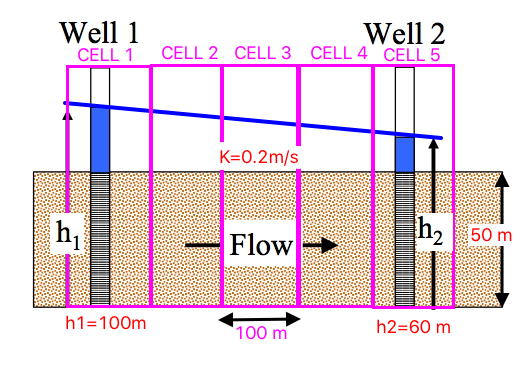
\includegraphics[width=4in]{./17-SteadyGroundwaterFlow/1D-aquifer-flow-fdm.jpg} 
   \caption{Schematic diagram of unidirectional flow in a generic aquifer, showing heads in two measuring wells.  The diagram is annotated with the cell spacing for the example (in magenta), as well as the cell ID.  The aquifer material properties are constant (K=0.2 m/s).   The head in the left well (Well 1) is 100 meters.   The head in the right well (Well 2) is 60 meters.}
   \label{fig:1D-aquifer-flow-fdm}
\end{figure}

Figure \ref{fig:1D-aquifer-flow-fdm} is the original sketch, annotated with cell spacing, material properties, and the head at the two wells.  In the figure, Well 1 has a head measurement of 100 meters, whereas Well 2 has a head measurement of 60 meters.  Because the flow is steady, and the material properties are spatially invariant, the EGL/HGL would be a line (the blue one in the figure) connecting the wells sloping from Well 1 to Well 2.

We will use the cell balance model to estimate the EGL/HGL in the aquifer (i.e. find the piezometric surface\footnote{Hydraulic head or piezometric head is a specific measurement of liquid pressure above a geodetic datum. It is usually measured as a liquid surface elevation, expressed in units of length, at the entrance (or bottom) of a piezometer. In an aquifer, it can be calculated from the depth to water in a piezometric well, and given information of the piezometer's elevation and screen depth.} between the two wells).

\begin{lstlisting}[caption=R code demonstrating an Aquifer Flow Simulator for Steady Flow \\ This fragment of code contains ..., label=lst:AquiferFlowSteady1Dimensional]
# 1D-confined-aquifer-steady-flow
# Implements Finite-Difference Porous Medium Flow using Jacobi Iteration
# Assumes boundary cells 1 and ncells are fixed head cells.
zz <- file("input1.dat", "r") # Open a connection named zz to file named input.dat
#
# read the simulation conditions
#
deltax <-as.numeric(readLines(zz, n = 1, ok = TRUE, warn = TRUE,encoding = "unknown", skipNul = FALSE))
deltay <-as.numeric(readLines(zz, n = 1, ok = TRUE, warn = TRUE,encoding = "unknown", skipNul = FALSE))
deltaz <-as.numeric(readLines(zz, n = 1, ok = TRUE, warn = TRUE,encoding = "unknown", skipNul = FALSE))
ncells <-as.numeric(readLines(zz, n = 1, ok = TRUE, warn = TRUE,encoding = "unknown", skipNul = FALSE))
tolerance <- as.numeric(readLines(zz, n = 1, ok = TRUE, warn = TRUE,encoding = "unknown", skipNul = FALSE))
hydhead <-(readLines(zz, n = 1, ok = TRUE, warn = TRUE,encoding = "unknown", skipNul = FALSE))
hydcond <-(readLines(zz, n = 1, ok = TRUE, warn = TRUE,encoding = "unknown", skipNul = FALSE))
close(zz)
#
# split the multiple column strings into numeric components for a vector
#
hydhead <-as.numeric(unlist(strsplit(hydhead,split=" ")))
hydcond <-as.numeric(unlist(strsplit(hydcond,split=" ")))
#
# built a position array for plotting
#
distance<-numeric(ncells)
distance[1]<-deltax/2.0
for (i in 2:ncells){distance[i]<-distance[i-1]+deltax}
#
# Plot Distance vs. Head before calculations
#
plot(distance,hydhead,col="red",xlim=c(0,deltax*ncells),ylim=c(0,max(hydhead)*2.0),pch=21,tck=1)
lines(distance,hydhead,col="red",type="l",lwd=3)
#
# built the transmissivity arrays
#
amat<-numeric(ncells) # make an ncells long array
bmat<-numeric(ncells) # make an ncells long array
for(irow in 2:(ncells-1)){
  amat[irow]<-((hydcond[irow-1]+hydcond[irow  ])*deltay*deltaz)/(2.0*deltax)
  bmat[irow]<-((hydcond[irow  ]+hydcond[irow+1])*deltay*deltaz)/(2.0*deltax)
}
#
# #se Jacobi iteration to find a solution to the difference equations
# 
headold<-hydhead # copy the head array, used to test for stopping 
maxit <- 100 # set the maximum number of iterations (to prevent infinite loop)
for (iter in 1:maxit){
  for (irow in 2:(ncells-1)){
    hydhead[irow]<-(amat[irow]*hydhead[irow-1]+bmat[irow]*hydhead[irow+1])/(amat[irow]+bmat[irow])
  }
# test for stopping iterations
  percentdiff <- sum((hydhead-headold)^2)
  if (percentdiff < tolerance){break}
  headold<-hydhead
}
#
# Add the steady-flow solution to the graph -- both points and a line.
#
lines(distance,hydhead,col="blue",type="p")
lines(distance,hydhead,col="blue",type="l",lwd=3)
\end{lstlisting}

Listing \ref{lst:AquiferFlowSteady1Dimensional} is a \textbf{R} script that reads an input file, computes the head distirbution (the ``blue line'') and plots the result.   The script also plots the initial values of the heads used in the computation engine.  Only the left most value and right most value remain unchanged as they represent the boundary conditions for the problem.

The iterative method is elementary for this case -- the replication of the head array at each step is used to test for stopping when the solution meets some tolerance.  The compute, test, update part of the script is a common structure in iterative problems, and when we modify the program for transient (time-varying) behavior it will come in handy.   There is no error trapping in the example -- so it is quite possible to supply an input file that would not work.  

Listing \ref{lst:1D-input-case1} is the contents of the input file (\texttt{input1.dat}) that is read by the script. 
To model different condtions, we would change the input file contents and leave the script alone.

\begin{lstlisting}[caption= Input File for Example Problem \\ This fragment of code contains ..., label=lst:1D-input-case1]
100
100
 50
5
1e-12
100 100 100 100 60
0.2 0.2 0.2 0.2 0.2
\end{lstlisting}

\begin{figure}[h!] %  figure placement: here, top, bottom, or page
   \centering
   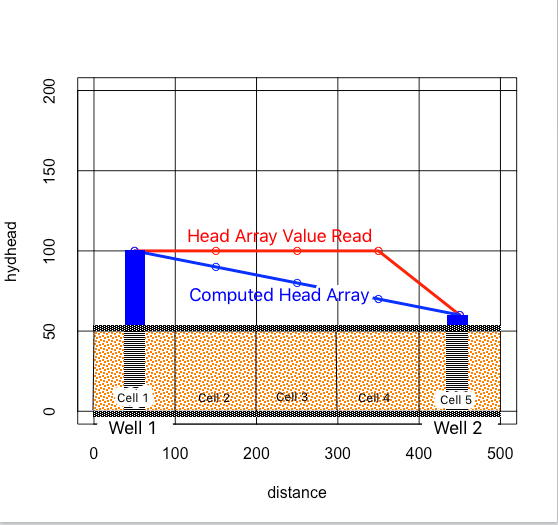
\includegraphics[width=4in]{./17-SteadyGroundwaterFlow/aquifer-1d-solution-case1.jpg} 
   \caption{Plot of computed head in each cell using Jacobi interation.   The head in the left well (Well 1) is 100 meters.   The head in the right well (Well 2) is 60 meters.  The steady flow solution is the blue line labelled ``Computed Head Array".}
   \label{fig:aquifer-1d-solution-case1}
\end{figure}
\newpage
Finally, for this problem Figure \ref{fig:aquifer-1d-solution-case1} is the output graphics from the script.  The red line is the value of heads supplied in the input file (these can be any values as long as the left and right values represent the conditions at the two wells); the blue line is the computed piezometric surface.  The markers are the computed head for each cell.

\textbf{Example 2: 1D Steady Flow in a Confined Aquifer using Gaussian Reduction}
The second example is the identical physical situation, but instead of iterative computations in our code, we will instead construct a simultaneous linear system ($Ax=b$) where the coefficient matrix $A$ is constructed from the difference equations and solved simultaneously.   

First we have to specify how to construct the matrices -- essentially because $h_1$ and $h_5$ are known, there are only three unknowns in the 5-cell example.  So we will have a linear system with 3 equations and 3 unknowns.  Here is the linear system in the context of the development of the difference equations.

\begin{displaymath}
\footnotesize
\begin{matrix}
-(A_2+B_2)\times h_2  & B_2\times h_3 & 0 \times h_4&  = & -A_3 \times h_1\\
A_3 \times h_2& -(A_3+B_3) \times h_3& B_3 \times h_4&  = & 0\\
0 \times h_2 & A_4 \times h_3 & -(A_4+B_4) \times h_4 & = & - B_4 \times h_5\\
 \end{matrix}
 \normalsize
 \end{displaymath}
 
 A more compact representation is
 \begin{displaymath}
\footnotesize
\begin{pmatrix}
-(A_2+B_2)  & B_2 & 0 \\
A_3 & -(A_3+B_3) & B_3 \\
0 & A_4 & -(A_4+B_4) \\
 \end{pmatrix}
 \begin{pmatrix}
 h_2 \\ h_3 \\ h_4 \\
 \end{pmatrix}
 =
  \begin{pmatrix}
 -A_3  h_1 \\ 0 \\ - B_4  h_5 \\
 \end{pmatrix}
 \normalsize
 \end{displaymath}
 Recall that the values for the coefficient matrix are known, as are the values $h_1$ and $h_5$.
 Now we will modify the script, to use the linear system solver and dispense with the iteration entirely.
 
 The modification(s) are to read in the values for the material and spatial properties -- just use the same code.  
 Then construct the compact matrix-vector equation by careful looping on the index values. 
 In the 5 cell example, only the inner three cells [2-4] are part of the linear system. 
 So we use indexing in the arithmetic to build the coefficient matrix and right-hand-side.
 
 Then when we have the solution, we need to put the computed values back into their correct position in the head vector.
 Listing \ref{lst:AquiferFlowSteady1DimensionalLinearSys} is a code listing that performs the various tasks.
 The script is intentionally built to use the same input file as the prior example. 
 
 The computed results are identical (as anticipated).  
 The next step (and the point of building such tools) is to try different spatial sizing (partly to be sure the code is generic and automatically adapts to such changes), and to apply the tool to aquifers with different material properties.

\clearpage 
 \begin{lstlisting}[caption= R code demonstrating an Aquifer Flow Simulator for Steady Flow  \\ 
 This version constructs coefficient matrix then solves the linear system. The program uses the same input
 file, label=lst:AquiferFlowSteady1DimensionalLinearSys]
# 1D-confined-aquifer-steady-flow
# Implements Finite-Difference Porous Medium Flow using Gaussian reduction
# Assumes boundary cells 1 and ncells are fixed head cells.
zz <- file("input1.dat", "r") # Open a connection named zz to file named input.dat
# read the simulation conditons
deltax <-as.numeric(readLines(zz, n = 1, ok = TRUE, warn = TRUE,encoding = "unknown", skipNul = FALSE))
deltay <-as.numeric(readLines(zz, n = 1, ok = TRUE, warn = TRUE,encoding = "unknown", skipNul = FALSE))
deltaz <-as.numeric(readLines(zz, n = 1, ok = TRUE, warn = TRUE,encoding = "unknown", skipNul = FALSE))
ncells <-as.numeric(readLines(zz, n = 1, ok = TRUE, warn = TRUE,encoding = "unknown", skipNul = FALSE))
tolerance <- as.numeric(readLines(zz, n = 1, ok = TRUE, warn = TRUE,encoding = "unknown", skipNul = FALSE))
hydhead <-(readLines(zz, n = 1, ok = TRUE, warn = TRUE,encoding = "unknown", skipNul = FALSE))
hydcond <-(readLines(zz, n = 1, ok = TRUE, warn = TRUE,encoding = "unknown", skipNul = FALSE))
close(zz)
# split the multiple column strings into numeric components for a vector
hydhead <-as.numeric(unlist(strsplit(hydhead,split=" ")))
hydcond <-as.numeric(unlist(strsplit(hydcond,split=" ")))

# built a position array for plotting
distance<-numeric(ncells)
distance[1]<-deltax/2.0
for (i in 2:ncells){distance[i]<-distance[i-1]+deltax}
plot(distance,hydhead,col="red",xlim=c(0,deltax*ncells),ylim=c(0,max(hydhead)*2.0),pch=21,tck=1)
lines(distance,hydhead,col="red",type="l",lwd=3)
# built the transmissivity arrays
amat<-numeric(ncells) # make an ncells long array
bmat<-numeric(ncells) # make an ncells long array
for(irow in 2:(ncells-1)){
  amat[irow]<-((hydcond[irow-1]+hydcond[irow  ])*deltay*deltaz)/(2.0*deltax)
  bmat[irow]<-((hydcond[irow  ]+hydcond[irow+1])*deltay*deltaz)/(2.0*deltax)
}
amatrix <- matrix(0,ncells-2,ncells-2)  # prefill matrix with zeros
rhs <- matrix(0,ncells-2)               # prefill vector with zeros
####################################################################
## build matrices here -- there are array indexing things going on #
## because we only have three equations to deal with.              #
## hydhead[1] is the left boundary                                 #
## hydhead[ncells] is the right boundary                           #
##  Only build the non-zero elements using the structure of the    #
##  difference-equation stencil (mask, computational molecule ...) #
####################################################################
## first row special
for (irow in 1:1){
  amatrix[irow,1]=-1.0*(amat[irow+1]+bmat[irow+1])
  amatrix[irow,2]=bmat[irow+1]
  rhs[irow] = -amat[irow+1]*hydhead[irow]
}
## interior rows
for (irow in 2:(ncells-3)){
  amatrix[irow,irow-1]=amat[irow+1] 
  amatrix[irow,irow]= -1.0*(amat[irow+1]+bmat[irow+1])
  amatrix[irow,irow+1]= bmat[irow+1]
}
## last row special
for (irow in (ncells-2):(ncells-2)){
  amatrix[irow,ncells-3]=amat[irow+1] 
  amatrix[irow,ncells-2]=-1.0*(amat[irow+1]+bmat[irow+1])
  rhs[irow] = -bmat[irow+1]*hydhead[irow+2]
}
####################################################################
## Now solve the linear system amatrix*unkvector=rhs for unkvector #
##  then put values from unkvector into correct position hydhead   #
####################################################################
unkvector<-solve(amatrix,rhs)
for (irow in 2:(ncells-1)){
  hydhead[irow] <- unkvector[irow-1]
}
###################################################################
## Plot the computed values in blue                               #
###################################################################
lines(distance,hydhead,col="blue",type="p")
lines(distance,hydhead,col="blue",type="l",lwd=3)
\end{lstlisting}
\clearpage
The next part of the example is what is the cell size is changed?  
The whole point of input files and such to to keep the script generic.  
So to check this situation, lets halve the space size (50 meters spacing, instead of 100 meters).
Thus instead of 5 cells of 100 meters each, we now have 5 cells of 50 meters each.
Listing \ref{lst:1D-input-case2} is a listing of what the input file looks like, other than twice as many initial heads and K values, essentially the same input.
\begin{lstlisting}[caption= Input File for Example Problem \\ , label=lst:1D-input-case2]
50 << changed cell size
100
 50
9 << more cells
1e-12
100 100 100 100 100 100 100 100 60 << more cells
0.2 0.2 0.2 0.2 0.2 0.2 0.2 0.2 0.2 0.2 << more cells
\end{lstlisting}

\begin{figure}[h!] %  figure placement: here, top, bottom, or page
   \centering
   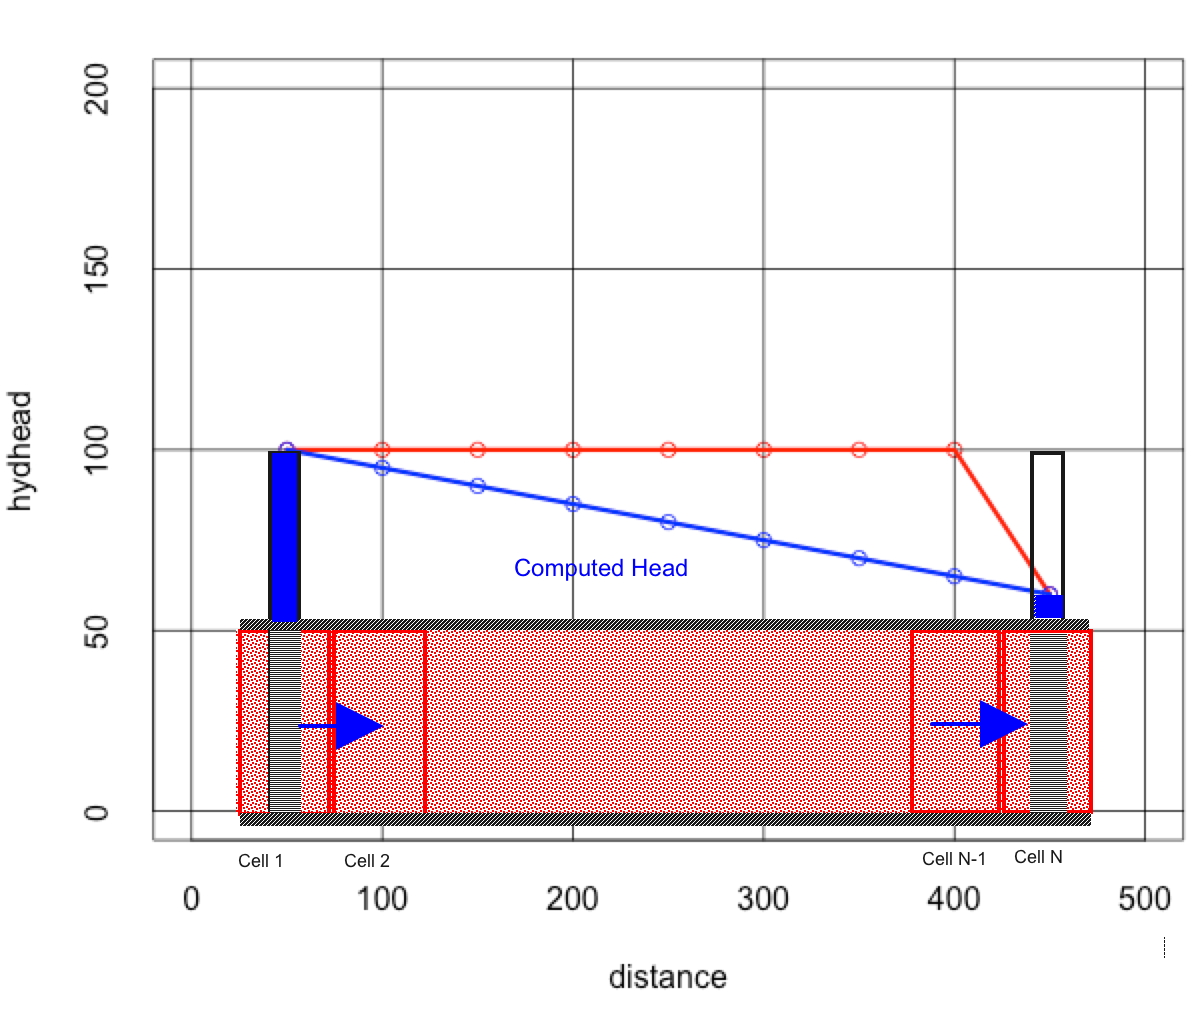
\includegraphics[width=4in]{./17-SteadyGroundwaterFlow/aquifer-1d-solution-case2.jpg} 
   \caption{Plot of computed head in each cell using different cell spacing.   The head in the left well (Well 1) is 100 meters.   The head in the right well (Well 2) is 60 meters.  The steady flow solution is the blue line labelled ``Computed Head Array".}
   \label{fig:aquifer-1d-solution-case2}
\end{figure}

Lastly, before we move to 2-Dimensional cases, lets examine when the material properties change.  
In this change, we will leave the first third of the aquifer with the same properties, but decrease hydraulic conductivity in the next third by 1/2 and the last third by 1/4 again.

Listing \ref{lst:1D-input-case3} is the input file for this case.  The anticipated result is that the HGL/EGL will change slope twice (starting out shallow, and getting steeper as we move to the right).
\clearpage
\begin{lstlisting}[caption= Input File for Example Problem \\ , label=lst:1D-input-case3]
50 
100
 50
9 << 
1e-12
100 100 100 100 100 100 100 100 60 << more cells
0.2 0.2 0.2 0.1 0.1 0.1 0.05 0.05 0.05 << more cells
\end{lstlisting}

Figure \ref{fig:aquifer-1d-solution-case3} is the results with this different input file and indeed as anticipated there are three different slopes (it looks like curvature on the plot, but its really just three different line segments with different slopes.).

\begin{figure}[h!] %  figure placement: here, top, bottom, or page
   \centering
   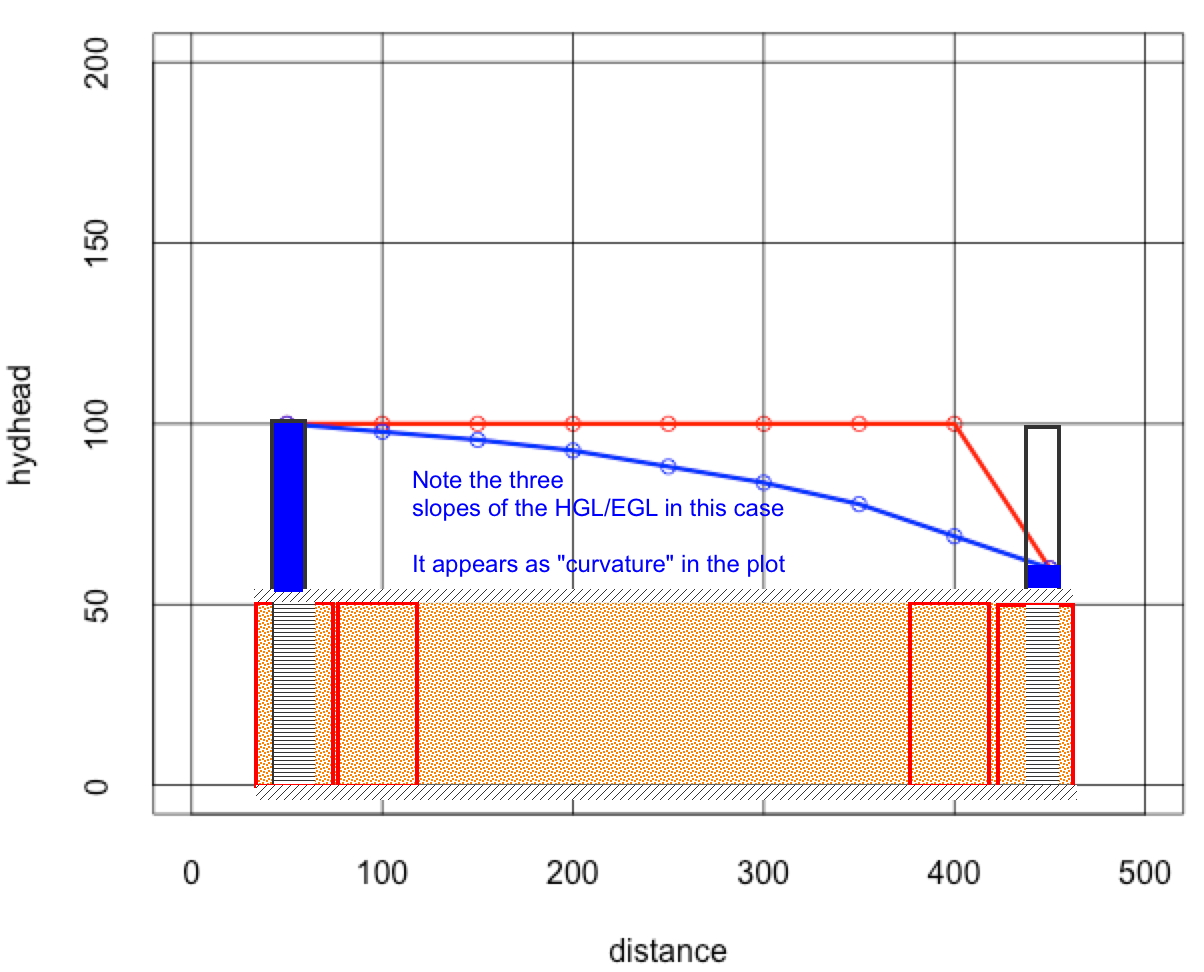
\includegraphics[width=4in]{./17-SteadyGroundwaterFlow/aquifer-1d-solution-case3.jpg} 
   \caption{Plot of computed head in each cell using different cell spacing.   The head in the left well (Well 1) is 100 meters.   The head in the right well (Well 2) is 60 meters.  The steady flow solution is the blue line.  The apparent curvature is really the three different slopes anticipated as the material properties change.}
   \label{fig:aquifer-1d-solution-case3}
\end{figure}
%%%%%%%%%%%%%%%%%%%%%%%%%%%%%%%%%%%%%%
%%%%%%%%%%%%%%%%%%%%%%%%%%%%%%%%%%%%%%
%%%%%%%%%%%%%%%%%%%%%%%%%%%%%%%%%%%%%%
\subsubsection{Finite-Difference Methods -- 2 Spatial Dimensions}
If we perform an analysis in the same way as we did to arrive at Equation \ref{eqn:confined-aquifer-flow-PDE} except now include another direction (the $y$-direction) we will have an aquifer in two spatial dimensions.  The governing equation becomes
  
\begin{equation}
S \frac{\partial h}{\partial t} = 
\frac{\partial}{\partial x}({T_x \frac{\partial h}{\partial x}})
+
\frac{\partial}{\partial y}({T_y \frac{\partial h}{\partial y}})
\label{eqn:confined-aquifer-flow-PDE2D}
\end{equation}

The meanings of the terms are the same, except the transmissivity terms now have subscripts to indicate they can have different values depending on direction.

Then as before we will construct the difference-equation model from a multiple-cell balance model of the aquifer at a cell of interest, then extend the equations to cover the entire model domain.

Figure \ref{fig:multiple-cell-balance-2d} is a plan view schematic of a aquifer with flow to be computed in two directions ($x$ and $y$).   The cell indexing convention in the sketch is that rows are indexed by the letter $j$ and columns are indexed by the letter $i$.  This naming convention is arbitrary; in some instances it may be preferable to reverse the convention.
The schematic also shows the assumed flow directions; for column $i$, flows are upward in the drawing, and for row $j$, flows are from left to right.  If indeed the opposite is true for a given set of boundary conditions and material properties, then the flows will be computed as negative numbers -- hence the convention here is that ``positive flow'' is right and up.  
\begin{figure}[h!] %  figure placement: here, top, bottom, or page
   \centering
   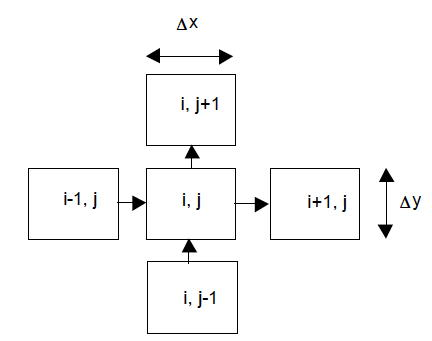
\includegraphics[width=4in]{./17-SteadyGroundwaterFlow/multiple-cell-balance-2d.jpg} 
   \caption{Plan view schematic of 2-dimensional multiple cell balance computational stencil}
   \label{fig:multiple-cell-balance-2d}
\end{figure}

As in the one-dimensional development the storage term is 
\begin{equation}
{\frac{d M_{water}}{dt}\mid}_{cell} =\rho_{w} S_{s} \Delta x \Delta y \Delta z \frac{\partial h_i}{\partial t}
\end{equation}
 where $h_i$ is the head in the $i-$th cell.  
 
 The mass flows entering the $i-\text{th},j-\text{th}$ cell are:
 \begin{equation}
M_{Inflow} = Q_{left} + Q_{bottom}=
\rho_{w} K_{x} \Delta y \Delta z \frac{h_{i-1,j} - h_{i,j}}{\Delta x} +
\rho_{w} K_{y} \Delta x \Delta z \frac{h_{i,j-1} - h_{i,j}}{\Delta y}                  
\end{equation}
 
The mass flows leaving the $i-\text{th},j-\text{th}$ cell are:
\begin{equation}
M_{Inflow} = Q_{right} + Q_{top}=
\rho_{w} K_{x} \Delta y \Delta z \frac{h_{i,j} - h_{i+1,j}}{\Delta x} +
\rho_{w} K_{y} \Delta x \Delta z \frac{h_{i,j} - h_{i,j+1}}{\Delta y}                  
\end{equation}

Now write the entire balance equation

\begin{equation}
\begin{matrix}
\rho_{w} S_{s} \Delta x \Delta y \Delta z \frac{\partial h_i}{\partial t} = 
[\rho_{w} K_{x} \Delta y \Delta z \frac{h_{i-1,j} - h_{i,j}}{\Delta x} +
\rho_{w} K_{y} \Delta x \Delta z \frac{h_{i,j-1} - h_{i,j}}{\Delta y}] - \\
~~~~~~~~~~\\
~~~~~~~~~~[\rho_{w} K_{x} \Delta y \Delta z \frac{h_{i,j} - h_{i+1,j}}{\Delta x} +
\rho_{w} K_{y} \Delta x \Delta z \frac{h_{i,j} - h_{i,j+1}}{\Delta y} ]        
\end{matrix}        
\end{equation}

Next replace $S_s \Delta z$ with the storage coefficient $S$, and the $K_{x,y} \Delta z$ with the transmissivity $T_{x,y}$ terms, and divide by the density of the fluid and the cell plan view area $\Delta x \Delta y$ to obtain a more compact form of the difference equation.

\begin{equation}
\begin{matrix}
S \frac{\partial h_i}{\partial t} = 
[\frac{1}{\Delta x} T_{x} \frac{h_{i-1,j} - h_{i,j}}{\Delta x} +
 \frac{1}{\Delta y} T_{y} \frac{h_{i,j-1} - h_{i,j}}{\Delta y}] - \\
~~~~~~~~~~\\
~~~~~~~~~~[ \frac{1}{\Delta x} T_{x}  \frac{h_{i,j} - h_{i+1,j}}{\Delta x} +
  \frac{1}{\Delta y}  T_{y} \frac{h_{i,j} - h_{i,j+1}}{\Delta y} ]        
\end{matrix}        
\end{equation}

As in the one-dimensional case, lets again consider steady flow (we will do transient flows later on)

\begin{equation}
\begin{matrix}
0= 
[\frac{1}{\Delta x} T_{x} \frac{h_{i-1,j} - h_{i,j}}{\Delta x} +
 \frac{1}{\Delta y} T_{y} \frac{h_{i,j-1} - h_{i,j}}{\Delta y}] - \\
~~~~~~~~~~\\
~~~~~~~~~~[ \frac{1}{\Delta x} T_{x}  \frac{h_{i,j} - h_{i+1,j}}{\Delta x} +
  \frac{1}{\Delta y}  T_{y} \frac{h_{i,j} - h_{i,j+1}}{\Delta y} ]        
\end{matrix}        
\end{equation}

Also as in the one-dimensional case, we will approximate the spatial variation of the material properties (transmissivity) as arithmetic mean values between two cells, so making the following definitions:

\begin{equation}
\begin{matrix}
A_{i,j} = \frac{1}{2 \Delta x^2}(T_{x,(i-1,j)}+T_{x,(i,j)}) \\ ~~ \\
B_{i,j} = \frac{1}{2 \Delta x^2}(T_{x,(i,j)}+T_{x,(i+1,j)})   \\ ~~ \\
C_{i,j} = \frac{1}{2 \Delta y^2}(T_{y,(i,j-1)}+T_{y,(i,j)})   \\ ~~ \\
D_{i,j} = \frac{1}{2 \Delta y^2}(T_{y,(i,j)}+T_{y,(i,j+1)})   \\ ~~ \\
\end{matrix}
\end{equation}

Substitution into the difference equation yields

\begin{equation}
0 = A_{i,j}h_{i-1,j} + B_{i,j}h_{i+1,j} - (A_{i,j}+B_{i,j}+C_{i,j}+D_{i,j})h_{i,j} + C_{i,j}h_{i,j-1} + D_{i,j}h_{i,j+1}
\end{equation}

As before we can explicitly write the cell equation for $h_{i,j}$ as

\begin{equation}
h_{i,j} = \frac{[A_{i,j}h_{i-1,j} + B_{i,j}h_{i+1,j} + C_{i,j}h_{i,j-1} + D_{i,j}h_{i,j+1}]}{[A_{i,j}+B_{i,j}+C_{i,j}+D_{i,j}]}
\end{equation}

This difference equation represents an approximation to the governing flow equation, the accuracy depending on the cell
size. Boundary conditions are applied directly into the analogs (another name for the difference equations) at appropriate
locations on the computational grid. Also as in the one-dimensional case we can generate solutions either by iteration or solving the resulting linear system.  

\textbf{Example 1: 2D Steady Flow in a Confined Aquifer using Jacobi Iteration}
As before we will start the example with a simple physical condition and use Jacobi iteration\footnote{Jacobi iteration for large domain problems (say 200x200) or bigger, is pretty inefficient -- better iterative methods are available; however they represent clever changes to the basic iteration methods explained here, hence Jacobi is a good place to start.} to obtain a solution.  
We will also incorporate two kinds of boundary conditions (fixed head as before, and no-flow boundaries).

Figure \ref{fig:aquifer-2d-layout} is a schematic of this example.   The right panel of the figure shows the index naming convention.  The known material properties are transmissivity (in each direction, at each cell center, and the thickness of the aquifer ($b == \Delta z$).
\begin{figure}[h!] %  figure placement: here, top, bottom, or page
   \centering
   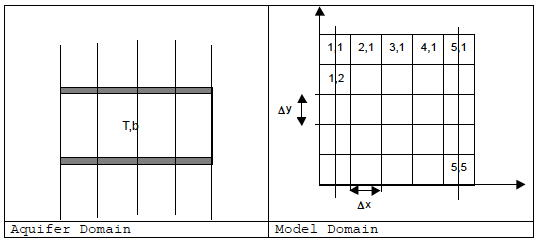
\includegraphics[width=6in]{./17-SteadyGroundwaterFlow/aquifer-2d-layout.jpg} 
   \caption{Schematic of 2-dimensional aquifer.  The left and right boundaries are constant head boundaries, whereas the upper and lower boundaries are no-flow}
   \label{fig:aquifer-2d-layout}
\end{figure}
Our task is to simulate the aquifer with the 5 x 5 model shown. 
The left and right boundaries will be treated as specified head boundaries. 
The upper and lower boundary will be treated as no flow boundaries.

The head on the left is 100 meters and the right is 60 meters (same as before).
The transmissivity ($K_{x,y} \Delta z$=10) square meters per second (but to be consistent with the earlier models we will supply a value of $K$ and $\Delta z$; keeping with the earlier examples the values are $K=0.2$ meters per second, and $\Delta z=50$ meters.
The spatial dimensions are $\Delta x = 100$ meters and $\Delta y = 100$ meters.

Listing \ref{lst:2D-Jacobi} is a listing that implements the method -- in this case there are changes to the data reading (to read and build matrices), and notice how the no-flow boundary conditions are implemented.   
\begin{lstlisting}[caption= R code demonstrating an Aquifer Flow Simulator for 2D Steady Flow.  This code fragment implements the Jacobi iteration.  A subsequent listing shows the contour plot syntax.  In the example the two fragments are joined and run as a single source file \\ , label=lst:2D-Jacobi]
# Implements 2D-Confined Aquifer Steady Flow Finite-Difference using Jacobi Iteration
# Assumes no-flow boundary row=1,and nrows.  Assumes fixed head boundary col=1, and ncols
# Head boundary conditions are entered in input file
zz <- file("input1.dat", "r") # Open a connection named zz to file named input.dat
# read the simulation conditons
deltax <-as.numeric(readLines(zz, n = 1, ok = TRUE, warn = TRUE,encoding = "unknown", skipNul = FALSE))
deltay <-as.numeric(readLines(zz, n = 1, ok = TRUE, warn = TRUE,encoding = "unknown", skipNul = FALSE))
deltaz <-as.numeric(readLines(zz, n = 1, ok = TRUE, warn = TRUE,encoding = "unknown", skipNul = FALSE))
nrows <-as.numeric(readLines(zz, n = 1, ok = TRUE, warn = TRUE,encoding = "unknown", skipNul = FALSE))
ncols <-as.numeric(readLines(zz, n = 1, ok = TRUE, warn = TRUE,encoding = "unknown", skipNul = FALSE))
tolerance <- as.numeric(readLines(zz, n = 1, ok = TRUE, warn = TRUE,encoding = "unknown", skipNul = FALSE))
hydhead <-(readLines(zz, n = nrows, ok = TRUE, warn = TRUE,encoding = "unknown", skipNul = FALSE))
hydcondx <-(readLines(zz, n = nrows, ok = TRUE, warn = TRUE,encoding = "unknown", skipNul = FALSE))
hydcondy <-(readLines(zz, n = nrows, ok = TRUE, warn = TRUE,encoding = "unknown", skipNul = FALSE))
close(zz)
# split the multiple column strings into numeric components for a vector
hydhead <-as.numeric(unlist(strsplit(hydhead,split=" ")))
hydcondx <-as.numeric(unlist(strsplit(hydcondx,split=" ")))
hydcondy <-as.numeric(unlist(strsplit(hydcondy,split=" ")))
# convert the numeric vectors into matrices for easier indexing
hydhead <-matrix(hydhead,nrow=nrows,ncol=ncols,byrow = TRUE)
hydcondx <-matrix(hydcondx,nrow=nrows,ncol=ncols,byrow = TRUE)
hydcondy <-matrix(hydcondy,nrow=nrows,ncol=ncols,byrow = TRUE)
# built the transmissivity arrays
amat<-matrix(0,nrows,ncols) 
bmat<-matrix(0,nrows,ncols) 
cmat<-matrix(0,nrows,ncols)
dmat<-matrix(0,nrows,ncols)
for(irow in 2:(nrows-1)){
  for(jcol in 2:(ncols-1)){
amat[irow,jcol]<-((hydcondx[irow-1,jcol  ]+hydcondx[irow  ,jcol  ])*deltaz)/(2.0*deltax^2)
bmat[irow,jcol]<-((hydcondx[irow  ,jcol  ]+hydcondx[irow+1,jcol  ])*deltaz)/(2.0*deltax^2)
cmat[irow,jcol]<-((hydcondy[irow  ,jcol-1]+hydcondy[irow  ,jcol  ])*deltaz)/(2.0*deltay^2)
dmat[irow,jcol]<-((hydcondy[irow  ,jcol  ]+hydcondy[irow  ,jcol+1])*deltaz)/(2.0*deltay^2)
  }
}
headold<-hydhead # copy the head array, used to test for stopping 
maxit <- 100 # set the maximum number of iterations (to prevent infinite loop)
for (iter in 1:maxit){
  # first and last row special == no flow boundaries
  for(jcol in 1:ncols){
    hydhead[1,jcol]=hydhead[2,jcol]
    hydhead[nrows,jcol]=hydhead[nrows-1,jcol]
  }
  for (irow in 2:(nrows-1)){
    for (jcol in 2:(nrows-1)){
      hydhead[irow,jcol] = 
        (amat[irow,jcol]*hydhead[irow-1,jcol  ] +
         bmat[irow,jcol]*hydhead[irow+1,jcol  ] +
         cmat[irow,jcol]*hydhead[irow  ,jcol-1] +
         dmat[irow,jcol]*hydhead[irow  ,jcol+1]  )/
        (amat[irow,jcol]+bmat[irow,jcol]+cmat[irow,jcol]+dmat[irow,jcol])
    }
  }
# test for stopping iterations
  percentdiff <- sum((hydhead-headold)^2)
  if (percentdiff < tolerance){
    message("Exit iterations because tolerance met")
    break}
  headold<-hydhead  #update the current head vector
}\end{lstlisting}
\clearpage

Instead of line plots, the built-in contouring algorithm in \textbf{R} is used to render the output plot(s).  Listing \ref{lst:2D-Contour} is the script that generates a contour plot.  The rows are actually plotted in the vertical, and columns in the horizontal, so the plot is rotated relative to the definition sketch.\footnote{This kind of plotting is a hold-over from line-printer days, where the long axis would be oriented to the vertical so that it could print to its heart's content and still fit on the paper. Older tractor-feed line-printers could print 135 characters wide, and as long as the paper roll held out.  The paper was called green-bar; each perforated sheet was 11x17 and the sheets were connected.  Essentially the paper length was functionally infinite, but the width was fixes at 17 inches.}

\begin{lstlisting}[caption= R code demonstrating building a contour plot from the computed head distribution \\ , label=lst:2D-Contour]
##############################################################
###    built position arrays for contour plotting          ###
##############################################################
distancex<-numeric(nrows)
distancey<-numeric(ncols)
distancex[1]<-50
distancey[1]<-50
for (irow in 2:nrows){distancex[irow]<-distancex[irow-1]+deltax}
for (jcol in 2:ncols){distancey[jcol]<-distancey[jcol-1]+deltay}
##############################################################
###    contour plot of head -- note axes are rotated       ###
##############################################################
contour(distancex,distancey,hydhead,
        plot.title = title(main = "Steady 2D Aquifer Model (Head in Meters)",
                           xlab = "Meters (Y axis) ====>>", 
                           ylab = "Meters (X axis) ====>>"))
\end{lstlisting}

Listing \ref{lst:2D-input-case1} is a listing of the input file.  The only major change from the one-dimensional examples is the entire head and transmissivity arrays are supplied.  

\begin{lstlisting}[caption= Input File for Example Problem \\ , label=lst:2D-input-case1]
100
100
 50
5
5
1e-12
100 100 100 100 60
100 100 100 100 60
100 100 100 100 60
100 100 100 100 60
100 100 100 100 60
0.2 0.2 0.2 0.2 0.2
0.2 0.2 0.2 0.2 0.2
0.2 0.2 0.2 0.2 0.2
0.2 0.2 0.2 0.2 0.2
0.2 0.2 0.2 0.2 0.2
\end{lstlisting}

\begin{figure}[h!] %  figure placement: here, top, bottom, or page
   \centering
   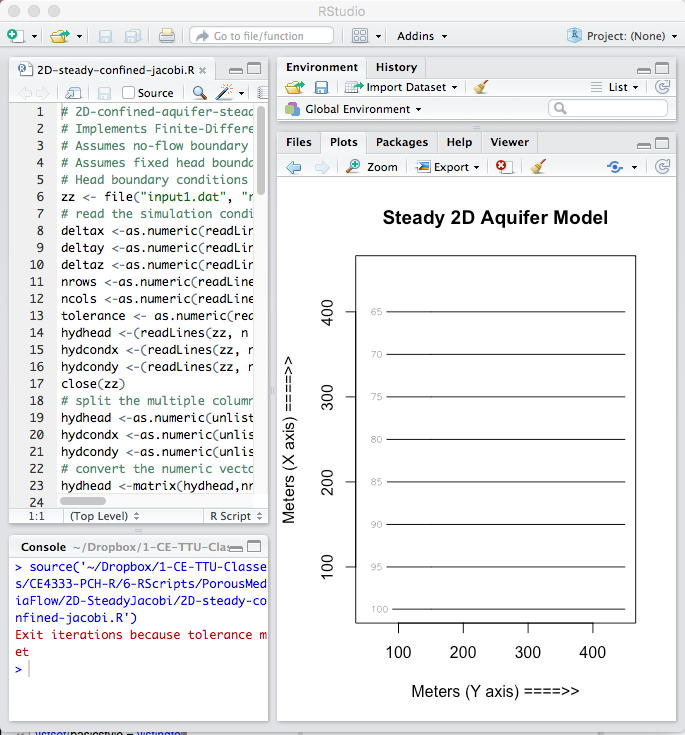
\includegraphics[height=6in]{./17-SteadyGroundwaterFlow/aquifer-2d-contour1.jpg} 
   \caption{Output from \textbf{R} script for 2D model.  Observe how the X-axis is plotted upward, and the Y-axis is plotter left to right.  The plotting is because of how ROWS and COLUMNS were indexed in the script.  Rather than alter the script, I find it easier to rotate the problem for practical application.}
   \label{fig:aquifer-2d-contour1}
\end{figure}
Figure \ref{fig:aquifer-2d-contour1} is a screen capture of the \textbf{R} output (using the R studio IDE).   The plot is on the right side of the screen image.
Figure \ref{fig:aquifer-2d-contour2} is a screen capture of just the plot, rotated, and with the boundaries identified (no-flow top and bottom; fixed head left and right).

\begin{figure}[h!] %  figure placement: here, top, bottom, or page
   \centering
   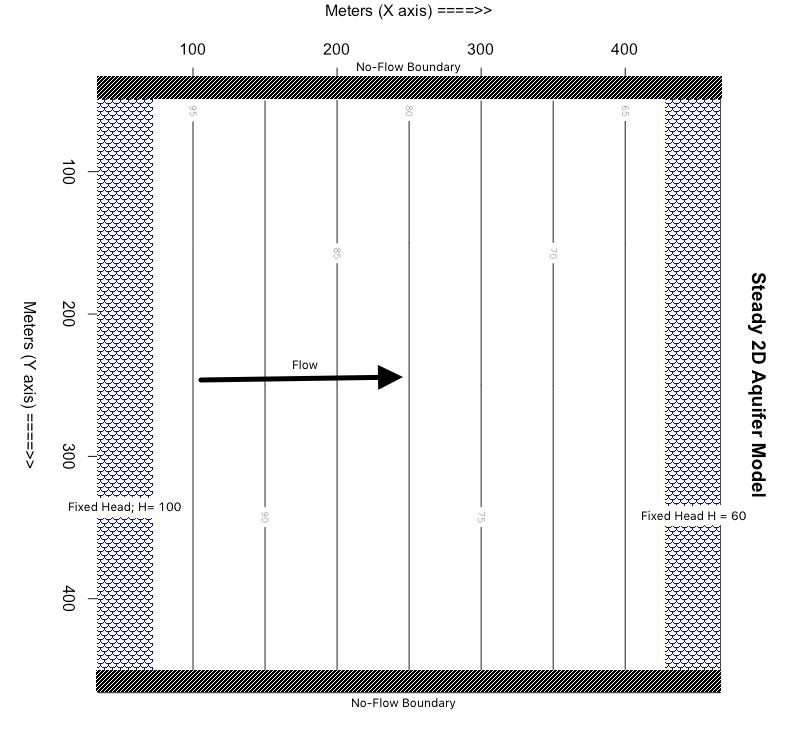
\includegraphics[height=6in]{./17-SteadyGroundwaterFlow/aquifer-2d-contour2.jpg} 
   \caption{Output from \textbf{R} script for 2D model, rotated and annotated to fit the original problem statement}
   \label{fig:aquifer-2d-contour2}
\end{figure}

Inspection of the script shows that there are still some parts of the script that could use generalization (namely the graphics portion, and a more sophisticated approach to boundary conditions), but otherwise we have the beginnings of a useful tool.   
To demonstrate the utility, lets change the input file to represent a different problem.
\clearpage

\textbf{Example 3: 2D Vertical Slice in a Confined Aquifer using Jacobi Iteration with Low Permeability Inclusion}

Figure \ref{fig:aquifer-2d-lowKinclusion} is a schematic of a different situation that now only requires us to change the contents of the data file, and re-run the scripts unchanged.  
Some additional modifications have been added, mostly messages to the user because of anticipated long run times.    
The data file is changed a bit and two lines are added to help with the plotting -- they represent the axis labels used in the contour plots.
The boundary conditions are still directly coded into the algorithm, and that would be the next modification to the code - general boundary condition information.\footnote{That modification is left for homework.}

\begin{figure}[h!] %  figure placement: here, top, bottom, or page
   \centering
   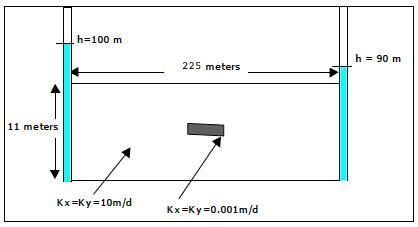
\includegraphics[width=4.5in]{./17-SteadyGroundwaterFlow/aquifer-2d-lowKinclusion.jpg} 
   \caption{Schematic of vertical slice in an aquifer with low permeability inclusion.  Values are indicated on the schematic }
   \label{fig:aquifer-2d-lowKinclusion}
\end{figure}

The following pages contain the code fragments (listings) for the head calculations, and the contour plotting.  As above, these listings are combined into a single file (the fragmentation herein is to fit the printed page layout) and then run as a script. 

Listing \ref{lst:2DinclusionHead} is the listing for the head calculations.  
Listing \ref{lst:2DinclusionHeadPlot} is the is the listing for the plotting calculations.
Listing \ref{lst:2DinclusionInput} is the input file for the problem.  
The file in this case is named \texttt{input2.dat}.  

In addition the generalized boundary conditions, the reader should consider making the program prompt the user for the file name, so that the program is more deployable.
Once a generalized boundary condition component is incorporated as well as a file prompt, the script would be useful in many practical situations.   
When we add wells to the governing PDE the tool would be quite relevant for engineering calculations.
\clearpage

\begin{lstlisting}[caption= 2D Steady Confined Aquifer Flow Script , label=lst:2DinclusionHead]
# 2D Aquifer Flow Model using Jacobi Iteration
# deallocate memory
rm(list=ls())
zz <- file("input2.dat", "r") # Open a connection named zz to file named input.dat
# read the simulation conditons
deltax <-as.numeric(readLines(zz, n = 1, ok = TRUE, warn = TRUE,encoding = "unknown", skipNul = FALSE))
deltay <-as.numeric(readLines(zz, n = 1, ok = TRUE, warn = TRUE,encoding = "unknown", skipNul = FALSE))
deltaz <-as.numeric(readLines(zz, n = 1, ok = TRUE, warn = TRUE,encoding = "unknown", skipNul = FALSE))
nrows <-as.numeric(readLines(zz, n = 1, ok = TRUE, warn = TRUE,encoding = "unknown", skipNul = FALSE))
ncols <-as.numeric(readLines(zz, n = 1, ok = TRUE, warn = TRUE,encoding = "unknown", skipNul = FALSE))
tolerance <- as.numeric(readLines(zz, n = 1, ok = TRUE, warn = TRUE,encoding = "unknown", skipNul = FALSE))
maxiter <- as.numeric(readLines(zz, n = 1, ok = TRUE, warn = TRUE,encoding = "unknown", skipNul = FALSE))
distancex <- (readLines(zz, n = 1, ok = TRUE, warn = TRUE,encoding = "unknown", skipNul = FALSE))
distancey <- (readLines(zz, n = 1, ok = TRUE, warn = TRUE,encoding = "unknown", skipNul = FALSE))
hydhead <-(readLines(zz, n = nrows, ok = TRUE, warn = TRUE,encoding = "unknown", skipNul = FALSE))
hydcondx <-(readLines(zz, n = nrows, ok = TRUE, warn = TRUE,encoding = "unknown", skipNul = FALSE))
hydcondy <-(readLines(zz, n = nrows, ok = TRUE, warn = TRUE,encoding = "unknown", skipNul = FALSE))
close(zz)
# split the multiple column strings into numeric components for a vector
distancex <-as.numeric(unlist(strsplit(distancex,split=" ")))
distancey <-as.numeric(unlist(strsplit(distancey,split=" ")))
hydhead <-as.numeric(unlist(strsplit(hydhead,split=" ")))
hydcondx <-as.numeric(unlist(strsplit(hydcondx,split=" ")))
hydcondy <-as.numeric(unlist(strsplit(hydcondy,split=" ")))
# convert the numeric vectors into matrices for easier indexing
hydhead <- matrix(hydhead,nrow=nrows,ncol=ncols,byrow = TRUE)
hydcondx <-matrix(hydcondx,nrow=nrows,ncol=ncols,byrow = TRUE)
hydcondy <-matrix(hydcondy,nrow=nrows,ncol=ncols,byrow = TRUE)
# here we perform the velocity potential calculations
# built the transmissivity arrays
amat<-matrix(0,nrows,ncols) 
bmat<-matrix(0,nrows,ncols) 
cmat<-matrix(0,nrows,ncols)
dmat<-matrix(0,nrows,ncols)
for(irow in 2:(nrows-1)){
  for(jcol in 2:(ncols-1)){
    amat[irow,jcol]<-((hydcondx[irow-1,jcol  ]+hydcondx[irow  ,jcol  ])*deltaz)/(2.0*deltax^2)
    bmat[irow,jcol]<-((hydcondx[irow  ,jcol  ]+hydcondx[irow+1,jcol  ])*deltaz)/(2.0*deltax^2)
    cmat[irow,jcol]<-((hydcondy[irow  ,jcol-1]+hydcondy[irow  ,jcol  ])*deltaz)/(2.0*deltay^2)
    dmat[irow,jcol]<-((hydcondy[irow  ,jcol  ]+hydcondy[irow  ,jcol+1])*deltaz)/(2.0*deltay^2)
  }
}
headold <- hydhead # copy the head array, used to test for stopping 
tolflag <- FALSE
for (iter in 1:maxiter){
  # first and last row special == no flow boundaries
  for(jcol in 1:ncols){
    hydhead[1,jcol]<-hydhead[2,jcol]
    hydhead[nrows,jcol]<-hydhead[nrows-1,jcol]
  }
  for (irow in 2:(nrows-1)){
    for (jcol in 2:(ncols-1)){
      hydhead[irow,jcol] <- 
        (amat[irow,jcol]*hydhead[irow-1,jcol  ] +
           bmat[irow,jcol]*hydhead[irow+1,jcol  ] +
           cmat[irow,jcol]*hydhead[irow  ,jcol-1] +
           dmat[irow,jcol]*hydhead[irow  ,jcol+1]  )/
        (amat[irow,jcol]+bmat[irow,jcol]+cmat[irow,jcol]+dmat[irow,jcol])
    }
  }
  # test for stopping iterations
  percentdiff <- sum((hydhead-headold)^2)
  if (percentdiff < tolerance){
    message("Exit iterations in velocity potential because tolerance met");
    message("Iterations =", iter);
    tolflag <- TRUE
    break}
 headold<-hydhead  #update the current head vector
 if( iter %% 1000 == 0){message("Calculating in Potential Function ",iter," of ",maxiter, " iterations")}
}
if (tolflag == FALSE){message("Exit iterations in potential function at max iterations")}

}\end{lstlisting}

\begin{lstlisting}[caption= Contour plotting script , label=lst:2DinclusionHeadPlot]
##############################################################
###    built position arrays for contour plotting          ###
##############################################################
velocity_plt<-matrix(0,ncols,nrows) 
for( i in 1:nrows){
  for( j in 1:ncols){
    velocity_plt[j,i]=hydhead[i,j]
  }
}
##############################################################
###    contour plot of head -- note axes are rotated       ###
##############################################################
contour(distancex,distancey,velocity_plt,
        plot.title = title(main = "Head (Blue) Map",
                           xlab = "Meters (X axis) ====>>", 
                           ylab = "Meters (Y axis) ====>>"),
        col="blue",lwd=3,nlevels=20)
\end{lstlisting}

\begin{lstlisting}[caption= Input file for 2D vertical slice confined aquifer with low permeability inclusion.  The comments in the listing should be removed for running the program , label=lst:2DinclusionInput]
1
10
1
13
23
1e-16  ## Stopping Criterion
50000 ## Maximum Iterations
5 15 25 35 45 55 65 75 85 95 105 115 125 135 145 155 165 175 185 195 205 215 225
0.5 1.5 2.5 3.5 4.5 5.5 6.5 7.5 8.5 9.5 10.5 11.5 12.5
100 100 100 100 100 100 100 100 100 100 100 100 100 100 100 100 100 100 100 100 100 100 90
100 100 100 100 100 100 100 100 100 100 100 100 100 100 100 100 100 100 100 100 100 100 90
100 100 100 100 100 100 100 100 100 100 100 100 100 100 100 100 100 100 100 100 100 100 90
100 100 100 100 100 100 100 100 100 100 100 100 100 100 100 100 100 100 100 100 100 100 90
100 100 100 100 100 100 100 100 100 100 100 100 100 100 100 100 100 100 100 100 100 100 90
100 100 100 100 100 100 100 100 100 100 100 100 100 100 100 100 100 100 100 100 100 100 90
100 100 100 100 100 100 100 100 100 100 100 100 100 100 100 100 100 100 100 100 100 100 90
100 100 100 100 100 100 100 100 100 100 100 100 100 100 100 100 100 100 100 100 100 100 90
100 100 100 100 100 100 100 100 100 100 100 100 100 100 100 100 100 100 100 100 100 100 90
100 100 100 100 100 100 100 100 100 100 100 100 100 100 100 100 100 100 100 100 100 100 90
100 100 100 100 100 100 100 100 100 100 100 100 100 100 100 100 100 100 100 100 100 100 90
100 100 100 100 100 100 100 100 100 100 100 100 100 100 100 100 100 100 100 100 100 100 90
100 100 100 100 100 100 100 100 100 100 100 100 100 100 100 100 100 100 100 100 100 100 90
10 10 10 10 10 10 10 10 10 10 10 10 10 10 10 10 10 10 10 10 10 10 10
10 10 10 10 10 10 10 10 10 10 10 10 10 10 10 10 10 10 10 10 10 10 10
10 10 10 10 10 10 10 10 10 10 10 10 10 10 10 10 10 10 10 10 10 10 10
10 10 10 10 10 10 10 10 10 10 10 10 10 10 10 10 10 10 10 10 10 10 10
10 10 10 10 10 10 10 10 10 10 10 10 10 10 10 10 10 10 10 10 10 10 10
10 10 10 10 10 10 10 10 10 10 0.0001 0.0001 0.0001 10 10 10 10 10 10 10 10 10 10
10 10 10 10 10 10 10 10 10 10 0.0001 0.0001 0.0001 10 10 10 10 10 10 10 10 10 10
10 10 10 10 10 10 10 10 10 10 0.0001 0.0001 0.0001 10 10 10 10 10 10 10 10 10 10
10 10 10 10 10 10 10 10 10 10 10 10 10 10 10 10 10 10 10 10 10 10 10
10 10 10 10 10 10 10 10 10 10 10 10 10 10 10 10 10 10 10 10 10 10 10
10 10 10 10 10 10 10 10 10 10 10 10 10 10 10 10 10 10 10 10 10 10 10
10 10 10 10 10 10 10 10 10 10 10 10 10 10 10 10 10 10 10 10 10 10 10
10 10 10 10 10 10 10 10 10 10 10 10 10 10 10 10 10 10 10 10 10 10 10
10 10 10 10 10 10 10 10 10 10 10 10 10 10 10 10 10 10 10 10 10 10 10
10 10 10 10 10 10 10 10 10 10 10 10 10 10 10 10 10 10 10 10 10 10 10
10 10 10 10 10 10 10 10 10 10 10 10 10 10 10 10 10 10 10 10 10 10 10
10 10 10 10 10 10 10 10 10 10 10 10 10 10 10 10 10 10 10 10 10 10 10
10 10 10 10 10 10 10 10 10 10 10 10 10 10 10 10 10 10 10 10 10 10 10
10 10 10 10 10 10 10 10 10 10 0.0001 0.0001 0.0001 10 10 10 10 10 10 10 10 10 10
10 10 10 10 10 10 10 10 10 10 0.0001 0.0001 0.0001 10 10 10 10 10 10 10 10 10 10
10 10 10 10 10 10 10 10 10 10 0.0001 0.0001 0.0001 10 10 10 10 10 10 10 10 10 10
10 10 10 10 10 10 10 10 10 10 10 10 10 10 10 10 10 10 10 10 10 10 10
10 10 10 10 10 10 10 10 10 10 10 10 10 10 10 10 10 10 10 10 10 10 10
10 10 10 10 10 10 10 10 10 10 10 10 10 10 10 10 10 10 10 10 10 10 10
10 10 10 10 10 10 10 10 10 10 10 10 10 10 10 10 10 10 10 10 10 10 10
10 10 10 10 10 10 10 10 10 10 10 10 10 10 10 10 10 10 10 10 10 10 10
\end{lstlisting}

Lastly, the result of running the script on the input file is shown in figure \ref{fig:LowPInclusionOut}

\begin{figure}[h!] %  figure placement: here, top, bottom, or page
   \centering
   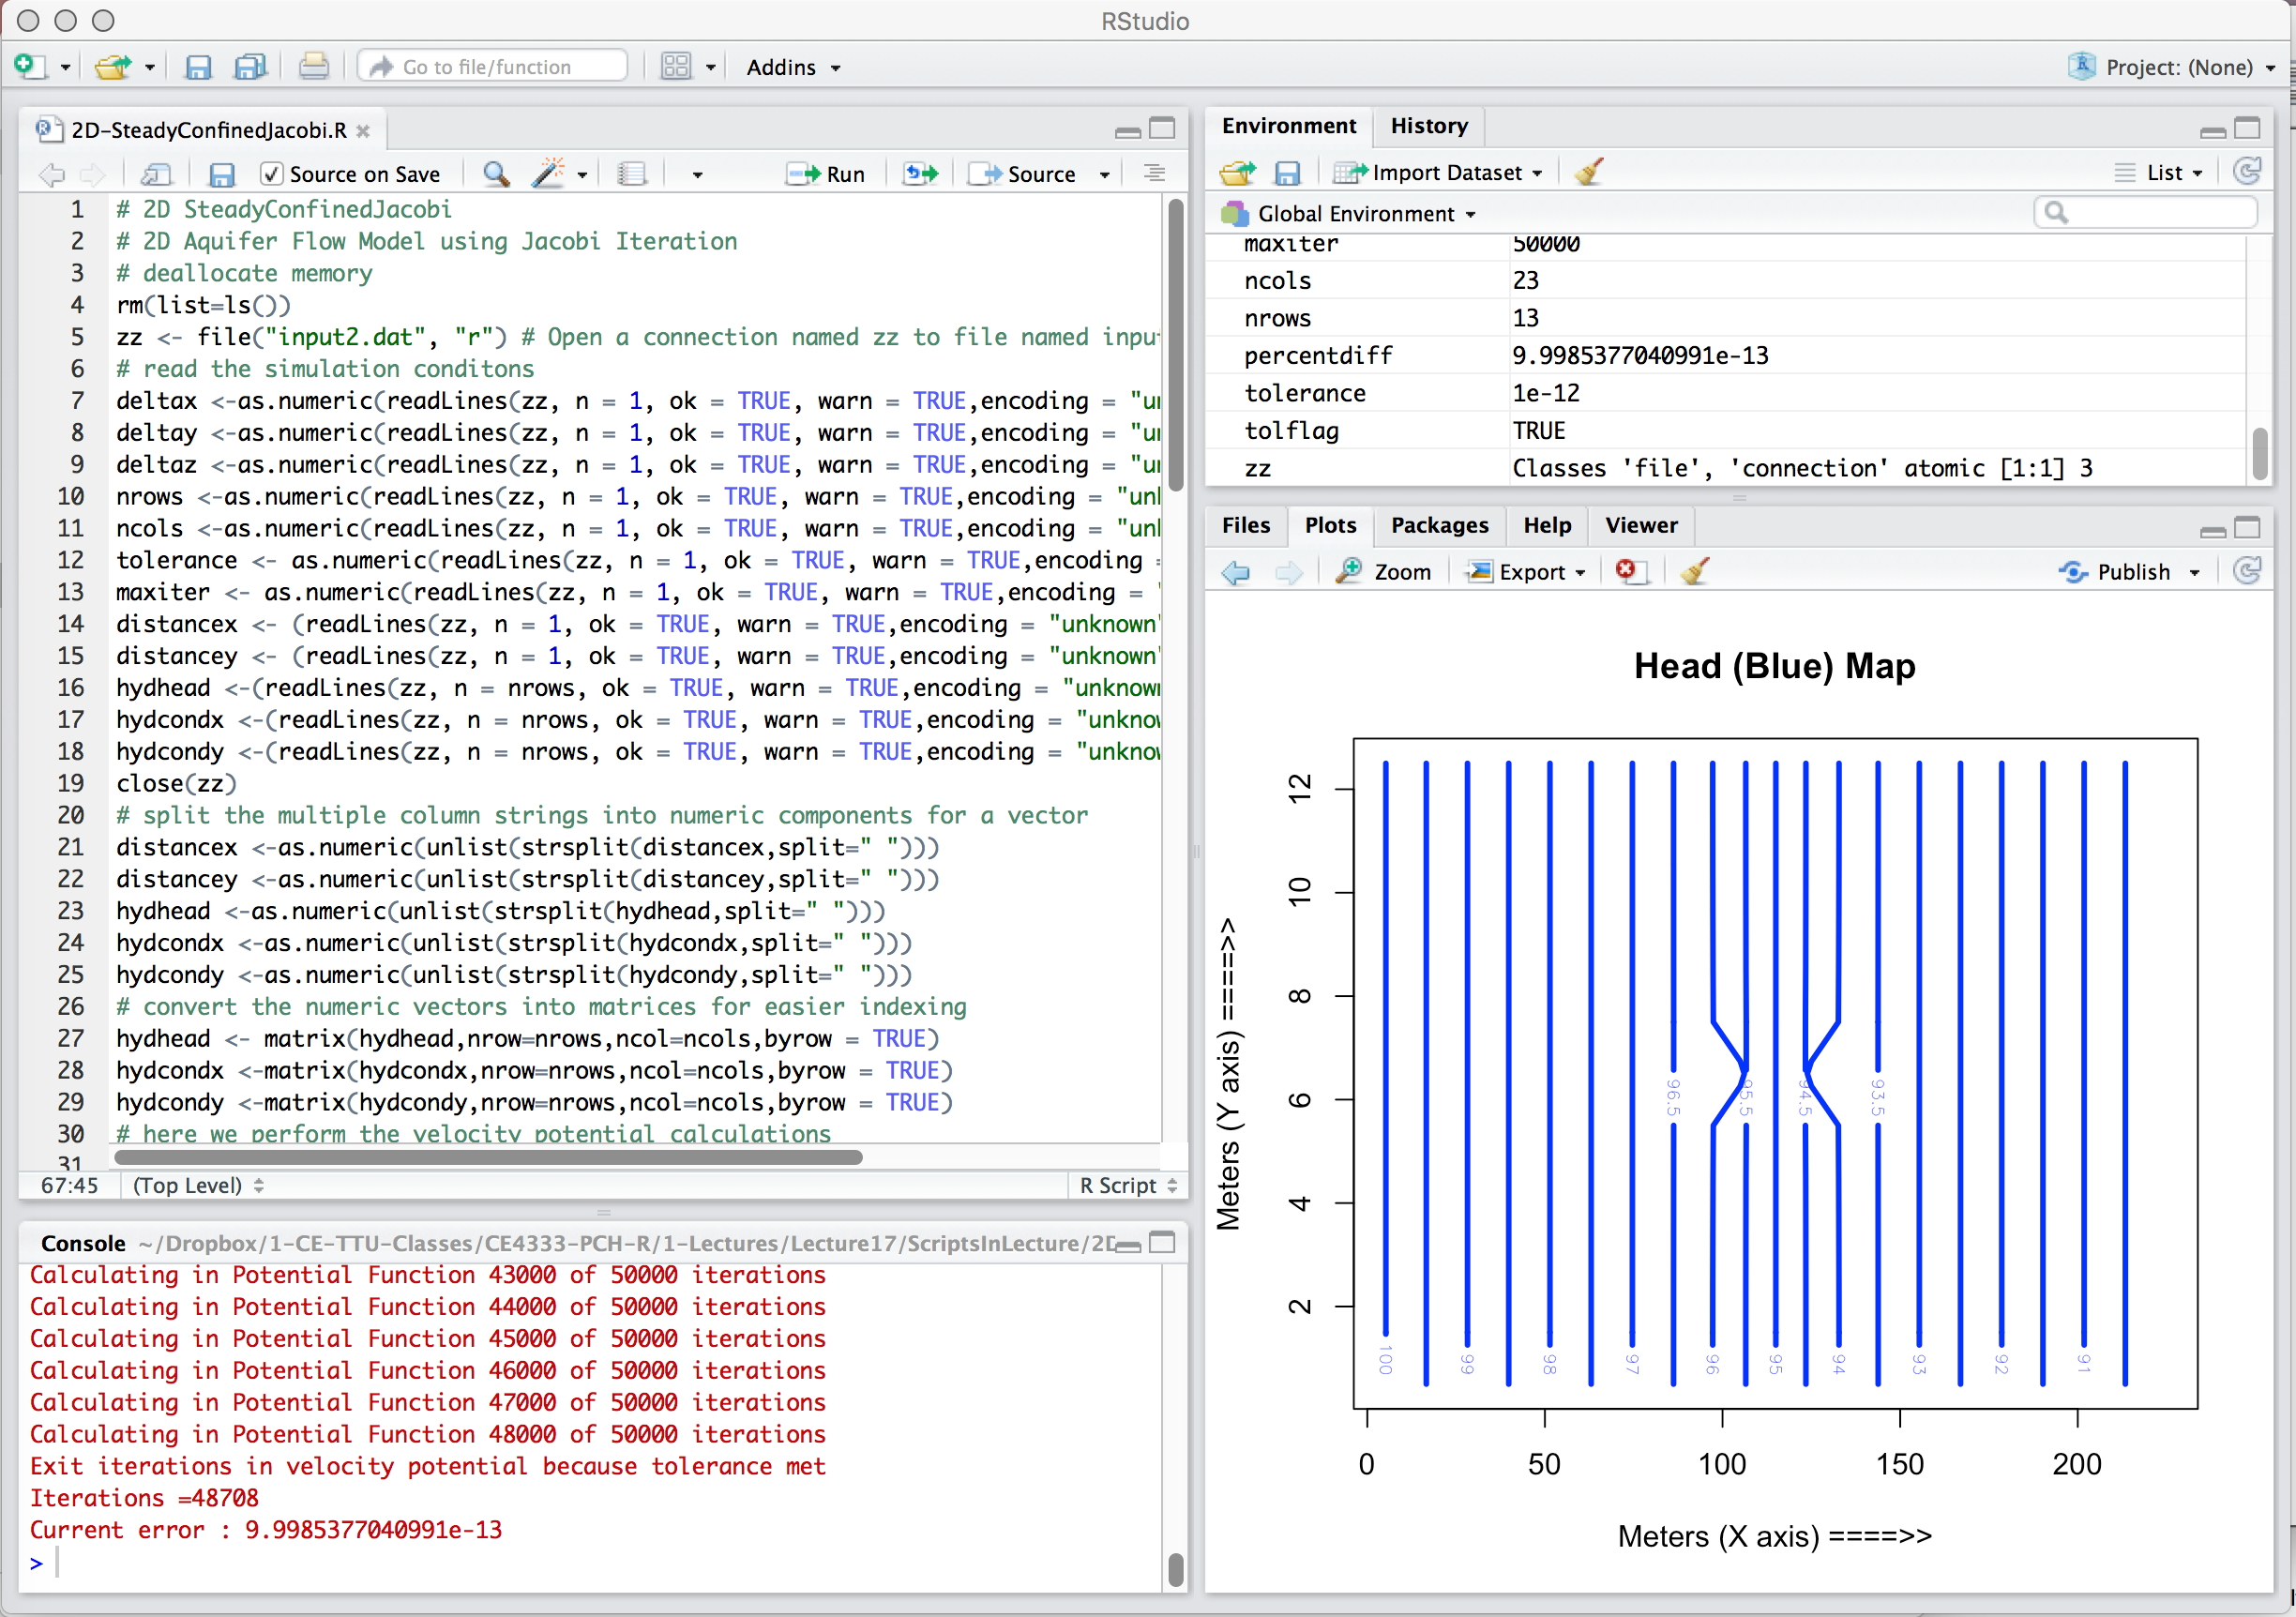
\includegraphics[width=5.2in]{./17-SteadyGroundwaterFlow/LowPInclusionOut.jpg} 
   \caption{Vertical slice in an aquifer with low permeability inclusion using Jacobi iteration scripts}
   \label{fig:LowPInclusionOut}
\end{figure}

Now when you run the script, it seems to take a long time and many iterations.  
This observation is indeed correct -- the ratio of conductivity terms and spatial discretization exerts a lot of influence on how fast the script can find a solution.
This problem exists for most iterative methods.  One could use the built-in \texttt{solve( \dots )} function, and simply solve the linear system without regard to structure, but assembly of the system matrix is non-trivial.\footnote{The system will be penta-diagional, and knowing this structure we could code a very efficient solver -- in this case we will use the built-in function, although we will tell the program that the matrix is sparse (e.g. \texttt{sparse = TRUE}) in the function call.}  
The head ``array'' would need to be addressed as a vector (we can use pointers to accomplish this task --- not too hard, but we would need to build the coefficient matrix, solve the system, and de-construct the result).   This task is saved for a future edition.

\subsubsection{Generalizing the Boundary Conditions}
In the prior examples the boundary conditions for the problems were kind of glossed over.
We applied a fixed head boundary on the left and right edges of the rectangular domain, and zero-flux boundary at the top and bottom edges.
A useful improvement is to allow the user to choose which type by supplying information in the input file.
I find the easiest way (as we are just learning) is to assume the entire model is always surrounded by a constant head condition and use a mask to tell the program when that is not true.  

The code fragments for making this change are pretty straightforward, and are displayed in Listing \ref{lst:BoundaryMask}.
We need to read in boundary indicators for the top, bottom, left, and right boundaries.  
Then convert them into numeric values for later.
Here I choose to use a zero to indicate a zero-flux boundary and any non-zero (usually a 1) to indicate a fixed head boundary.

Next we apply the conditions within the solver loop by assigning the compued value of the adjacent cell (either above, below, left, or right as appropriate).   
The reaminder of the script is unchanged, of coude we need to include the new input values in the data file as in Listing \ref{lst:BoundaryInputFile}.

\begin{lstlisting}[caption= Script fragments for implementing generalized boundary conditions , label=lst:BoundaryMask]
### Up in the input read section of the script ########
# add boundary conditions 0= fixed head, 1= no flow
boundarytop <- (readLines(zz, n = 1, ok = TRUE, warn = TRUE,encoding = "unknown", skipNul = FALSE))
boundarybottom <- (readLines(zz, n = 1, ok = TRUE, warn = TRUE,encoding = "unknown", skipNul = FALSE))
boundaryleft <- (readLines(zz, n = 1, ok = TRUE, warn = TRUE,encoding = "unknown", skipNul = FALSE))
boundaryright <- (readLines(zz, n = 1, ok = TRUE, warn = TRUE,encoding = "unknown", skipNul = FALSE))
hydhead <-(readLines(zz, n = nrows, ok = TRUE, warn = TRUE,encoding = "unknown", skipNul = FALSE))
.........
### Convert to numeric ######
boundarytop <-as.numeric(unlist(strsplit(boundarytop,split=" ")))
boundarybottom <-as.numeric(unlist(strsplit(boundarybottom,split=" ")))
boundaryleft <-as.numeric(unlist(strsplit(boundaryleft,split=" ")))
boundaryright <-as.numeric(unlist(strsplit(boundaryright,split=" ")))
...........
#### Apply the conditions ####
for (iter in 1:maxiter){
# Boundary Conditions
# Top and Bottom
for(jcol in 1:ncols){
    if(boundarytop[jcol] == 0){hydhead[1,jcol]<-hydhead[2,jcol]} #no-flow at top
    if(boundarybottom[jcol] == 0){hydhead[nrows,jcol]<-hydhead[2,jcol]} #no-flow at bottom
    # otherwise values are fixed head
}
for(irow in 1:nrows){
    if(boundaryleft[irow] == 0){hydhead[irow,1]<-hydhead[irow,2]} #no-flow at left
    if(boundaryright[irow] == 0){hydhead[irow,ncols]<-hydhead[irow,ncols-1]} #no-flow at right
    # otherwise values are fixed head
}
  for (irow in 2:(nrows-1)){ 
  ...........
  
\end{lstlisting}

\begin{lstlisting}[caption= Input file for 2D vertical slice confined aquifer with low permeability inclusion using a generalized boundary mask. The comments in the listing should be removed for running the program , label=lst:BoundaryInputFile]
1
10
1
13
23
1e-8
5000
5 15 25 35 45 55 65 75 85 95 105 115 125 135 145 155 165 175 185 195 205 215 225
0.5 1.5 2.5 3.5 4.5 5.5 6.5 7.5 8.5 9.5 10.5 11.5 12.5
0 0 0 0 0 0 0 0 0 0 0 0 0 0 0 0 0 0 0 0 0 0 0  # Boundary Conditions along Top
0 0 0 0 0 0 0 0 0 0 0 0 0 0 0 0 0 0 0 0 0 0 0  # Boundary Conditions along Bottom
1 1 1 1 1 1 1 1 1 1 1 1 1                      # Boundary Conditions along Left
1 1 1 1 1 1 1 1 1 1 1 1 1                      # Boundary Conditions along Right
100 100 100 100 100 100 100 100 100 100 100 100 100 100 100 100 100 100 100 100 100 100 100
100 100 100 100 100 100 100 100 100 100 100 100 100 100 100 100 100 100 100 100 100 100 100
100 100 100 100 100 100 100 100 100 100 100 100 100 100 100 100 100 100 100 100 100 100 100
100 100 100 100 100 100 100 100 100 100 100 100 100 100 100 100 100 100 100 100 100 100 100
100 100 100 100 100 100 100 100 100 100 100 100 100 100 100 100 100 100 100 100 100 100 100
100 100 100 100 100 100 100 100 100 100 100 100 100 100 100 100 100 100 100 100 100 100 100
100 100 100 100 100 100 100 100 100 100 100 100 100 100 100 100 100 100 100 100 100 100 100
100 100 100 100 100 100 100 100 100 100 100 100 100 100 100 100 100 100 100 100 100 100 100
100 100 100 100 100 100 100 100 100 100 100 100 100 100 100 100 100 100 100 100 100 100 100
100 100 100 100 100 100 100 100 100 100 100 100 100 100 100 100 100 100 100 100 100 100 100
100 100 100 100 100 100 100 100 100 100 100 100 100 100 100 100 100 100 100 100 100 100 100
100 100 100 100 100 100 100 100 100 100 100 100 100 100 100 100 100 100 100 100 100 100 100
100 100 100 100 100 100 100 100 100 100 100 100 100 100 100 100 100 100 100 100 100 100 100
10 10 10 10 10 10 10 10 10 10 10 10 10 10 10 10 10 10 10 10 10 10 10
10 10 10 10 10 10 10 10 10 10 10 10 10 10 10 10 10 10 10 10 10 10 10
10 10 10 10 10 10 10 10 10 10 10 10 10 10 10 10 10 10 10 10 10 10 10
10 10 10 10 10 10 10 10 10 10 10 10 10 10 10 10 10 10 10 10 10 10 10
10 10 10 10 10 10 10 10 10 10 10 10 10 10 10 10 10 10 10 10 10 10 10
10 10 10 10 10 10 10 10 10 10 0.001 0.001 0.001 10 10 10 10 10 10 10 10 10 10
10 10 10 10 10 10 10 10 10 10 0.001 0.001 0.001 10 10 10 10 10 10 10 10 10 10
10 10 10 10 10 10 10 10 10 10 0.001 0.001 0.001 10 10 10 10 10 10 10 10 10 10
10 10 10 10 10 10 10 10 10 10 10 10 10 10 10 10 10 10 10 10 10 10 10
10 10 10 10 10 10 10 10 10 10 10 10 10 10 10 10 10 10 10 10 10 10 10
10 10 10 10 10 10 10 10 10 10 10 10 10 10 10 10 10 10 10 10 10 10 10
10 10 10 10 10 10 10 10 10 10 10 10 10 10 10 10 10 10 10 10 10 10 10
10 10 10 10 10 10 10 10 10 10 10 10 10 10 10 10 10 10 10 10 10 10 10
10 10 10 10 10 10 10 10 10 10 10 10 10 10 10 10 10 10 10 10 10 10 10
10 10 10 10 10 10 10 10 10 10 10 10 10 10 10 10 10 10 10 10 10 10 10
10 10 10 10 10 10 10 10 10 10 10 10 10 10 10 10 10 10 10 10 10 10 10
10 10 10 10 10 10 10 10 10 10 10 10 10 10 10 10 10 10 10 10 10 10 10
10 10 10 10 10 10 10 10 10 10 10 10 10 10 10 10 10 10 10 10 10 10 10
10 10 10 10 10 10 10 10 10 10 0.001 0.001 0.001 10 10 10 10 10 10 10 10 10 10
10 10 10 10 10 10 10 10 10 10 0.001 0.001 0.001 10 10 10 10 10 10 10 10 10 10
10 10 10 10 10 10 10 10 10 10 0.001 0.001 0.001 10 10 10 10 10 10 10 10 10 10
10 10 10 10 10 10 10 10 10 10 10 10 10 10 10 10 10 10 10 10 10 10 10
10 10 10 10 10 10 10 10 10 10 10 10 10 10 10 10 10 10 10 10 10 10 10
10 10 10 10 10 10 10 10 10 10 10 10 10 10 10 10 10 10 10 10 10 10 10
10 10 10 10 10 10 10 10 10 10 10 10 10 10 10 10 10 10 10 10 10 10 10
10 10 10 10 10 10 10 10 10 10 10 10 10 10 10 10 10 10 10 10 10 10 10
\end{lstlisting}

Addition of the generalized boundary conditions expands the utility of our script as illustrated in the next example.\\

\textbf{Example 4: 2D Vertical Slice in for Computing Heads (Pore Pressure) under a Dam}

Figure \ref{fig:DamSeepage} is a schematic of a dam built upon a permeable ground layer 80 meters thick (segment A to I).  
The dam has a base 60 meters wide (segment B to F), with an upstream water depth of 10 meters.
The downstream side of the dam is at 0 meters depth (otherwise its not a very good dam!).  
A sheetpile cutoff wall is installed beneath the dam (segment C to D to U to E).   
The ground layer has a hydraulic conductivity of $K = 1 \times 10^{-4}$ meters per second.

\begin{figure}[h!] %  figure placement: here, top, bottom, or page
   \centering
   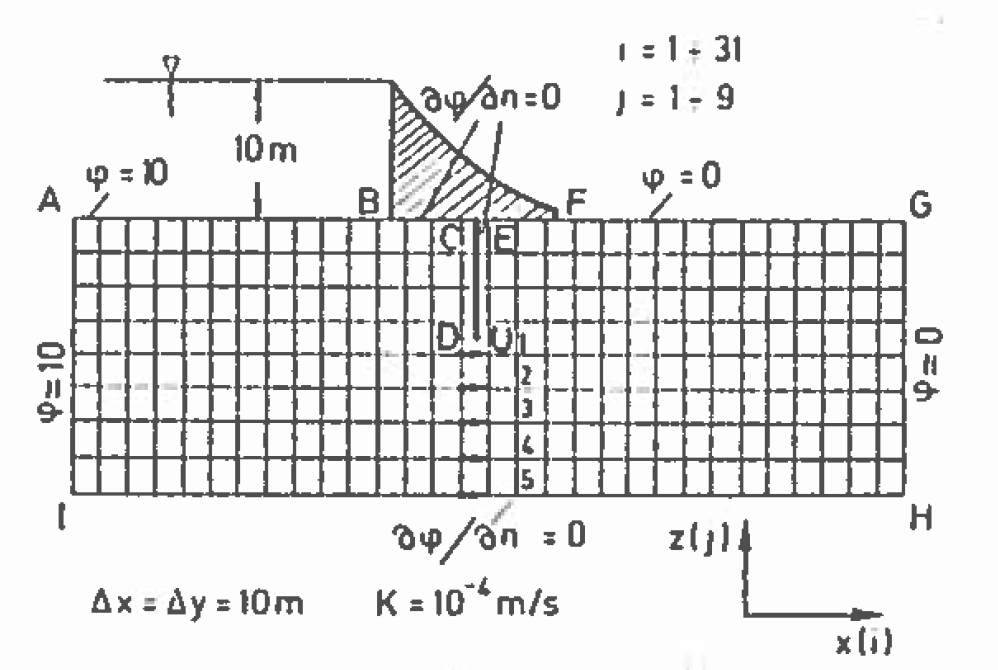
\includegraphics[width=5.2in]{./17-SteadyGroundwaterFlow/DamSeepage.jpg} 
   \caption{Schematic of a dam on permeable soil with the sheet pile curtain underneath the dam}
   \label{fig:DamSeepage}
\end{figure}
Important engineering questions are what is the pore water pressure under the dam, and is what is the total seepage under the dam?
The pore water pressure can be found by solving for heads under the dam then subtracting the elevation of the computation location elative to a datum.   
The flow is found by Darcy's law applied under the dam (shown as locations 1,2,3,4, and 5 in the sketch), which in turn requires computation of head under the dam.  
Thus the questions are answered by finding the head distribution under the dam.

The flow field (mathematically) extends an infinite distance upstream and downstream, but as a practical matter the contribution to seepage far upstream of the dam is negligible, and hence is approximated by the finite domain depicted.  

Using the tools we have already built we can simply build an input file, run our script and determine the head distribution (and thus compute the discharges under the dam.   There are two ways to conceptualize the model domain, we will examine both.  

The first is to represent the domain as shown, and make the following specifications in the boundary condition information, and we will treat the sheetpile cutoff wall as a low permeability inclusion (much like the the prior example).
The boundary conditions are:
\begin{enumerate}
\item The segment from A to B is a constant head boundary with value equal to 10.
\item The segment from B to F is a zero-flux boundary.
\item The segment from B to C to D to U to E to F should be treated as a zero-flux boundary, but our mask does not extend into the interior -- however the sheetpile itself can be approximated by providing a very small permeability.   Alternately we could (should) modify the code to handle interior boundaries -- but that is outside the scope of this chapter.
\item The segment from F to G is a constant head boundary with value equal to 0.
\item The segment form G to H is a constant head boundary with value equal to 0.
\item The segment from H to I is a zero-flux boundary.
\item The segment from I to A is a constant head boundary with value equal to 10.
\end{enumerate}

Listing \ref{lst:DamSeepage} is the input file that is used that incorporates the boundary conditions stated above.   
Observe how all we did was change the $\Delta x$ and $\Delta y$ specifications, modified the boundary condition arrays, and set the row and column counts.
\begin{lstlisting}[caption= Input file for 2D vertical slice for Dam Seepage Example , label=lst:DamSeepage]
10
10
1
9
31
1e-12
5000
0 10 20 30 40 50 60 70 80 90 100 110 120 130 140 150 160 170 180 190 200 210 220 230 240 250 260 270 280 290 300
0 10 20 30 40 50 60 70 80
1 1 1 1 1 1 1 1 1 1 1 1 0 0 0 0 0 0 1 1 1 1 1 1 1 1 1 1 1 1 1 
0 0 0 0 0 0 0 0 0 0 0 0 0 0 0 0 0 0 0 0 0 0 0 0 0 0 0 0 0 0 0 
1 1 1 1 1 1 1 1 1 
1 1 1 1 1 1 1 1 1 
10 10 10 10 10 10 10 10 10 10 10 10 10 10 10 0 0 0 0 0 0 0 0 0 0 0 0 0 0 0 0
10 10 10 10 10 10 10 10 10 10 10 10 10 10 10 0 0 0 0 0 0 0 0 0 0 0 0 0 0 0 0
10 10 10 10 10 10 10 10 10 10 10 10 10 10 10 0 0 0 0 0 0 0 0 0 0 0 0 0 0 0 0
10 10 10 10 10 10 10 10 10 10 10 10 10 10 10 0 0 0 0 0 0 0 0 0 0 0 0 0 0 0 0
10 10 10 10 10 10 10 10 10 10 10 10 10 10 10 0 0 0 0 0 0 0 0 0 0 0 0 0 0 0 0
10 10 10 10 10 10 10 10 10 10 10 10 10 10 10 0 0 0 0 0 0 0 0 0 0 0 0 0 0 0 0
10 10 10 10 10 10 10 10 10 10 10 10 10 10 10 0 0 0 0 0 0 0 0 0 0 0 0 0 0 0 0
10 10 10 10 10 10 10 10 10 10 10 10 10 10 10 0 0 0 0 0 0 0 0 0 0 0 0 0 0 0 0
10 10 10 10 10 10 10 10 10 10 10 10 10 10 10 0 0 0 0 0 0 0 0 0 0 0 0 0 0 0 0
0.0001 0.0001 0.0001 0.0001 0.0001 0.0001 0.0001 0.0001 0.0001 0.0001 0.0001 0.0001 0.0001 0.0001 0.0000001 0.0000001 0.0001 0.0001 0.0001 0.0001 0.0001 0.0001 0.0001 0.0001 0.0001 0.0001 0.0001 0.0001 0.0001 0.0001 0.0001
0.0001 0.0001 0.0001 0.0001 0.0001 0.0001 0.0001 0.0001 0.0001 0.0001 0.0001 0.0001 0.0001 0.0001 0.0000001 0.0000001 0.0001 0.0001 0.0001 0.0001 0.0001 0.0001 0.0001 0.0001 0.0001 0.0001 0.0001 0.0001 0.0001 0.0001 0.0001
0.0001 0.0001 0.0001 0.0001 0.0001 0.0001 0.0001 0.0001 0.0001 0.0001 0.0001 0.0001 0.0001 0.0001 0.0000001 0.0000001 0.0001 0.0001 0.0001 0.0001 0.0001 0.0001 0.0001 0.0001 0.0001 0.0001 0.0001 0.0001 0.0001 0.0001 0.0001
0.0001 0.0001 0.0001 0.0001 0.0001 0.0001 0.0001 0.0001 0.0001 0.0001 0.0001 0.0001 0.0001 0.0001 0.0000001 0.0000001 0.0001 0.0001 0.0001 0.0001 0.0001 0.0001 0.0001 0.0001 0.0001 0.0001 0.0001 0.0001 0.0001 0.0001 0.0001
0.0001 0.0001 0.0001 0.0001 0.0001 0.0001 0.0001 0.0001 0.0001 0.0001 0.0001 0.0001 0.0001 0.0001 0.0000001 0.0000001 0.0001 0.0001 0.0001 0.0001 0.0001 0.0001 0.0001 0.0001 0.0001 0.0001 0.0001 0.0001 0.0001 0.0001 0.0001
0.0001 0.0001 0.0001 0.0001 0.0001 0.0001 0.0001 0.0001 0.0001 0.0001 0.0001 0.0001 0.0001 0.0001 0.0001 0.0001 0.0001 0.0001 0.0001 0.0001 0.0001 0.0001 0.0001 0.0001 0.0001 0.0001 0.0001 0.0001 0.0001 0.0001 0.0001
0.0001 0.0001 0.0001 0.0001 0.0001 0.0001 0.0001 0.0001 0.0001 0.0001 0.0001 0.0001 0.0001 0.0001 0.0001 0.0001 0.0001 0.0001 0.0001 0.0001 0.0001 0.0001 0.0001 0.0001 0.0001 0.0001 0.0001 0.0001 0.0001 0.0001 0.0001
0.0001 0.0001 0.0001 0.0001 0.0001 0.0001 0.0001 0.0001 0.0001 0.0001 0.0001 0.0001 0.0001 0.0001 0.0001 0.0001 0.0001 0.0001 0.0001 0.0001 0.0001 0.0001 0.0001 0.0001 0.0001 0.0001 0.0001 0.0001 0.0001 0.0001 0.0001
0.0001 0.0001 0.0001 0.0001 0.0001 0.0001 0.0001 0.0001 0.0001 0.0001 0.0001 0.0001 0.0001 0.0001 0.0001 0.0001 0.0001 0.0001 0.0001 0.0001 0.0001 0.0001 0.0001 0.0001 0.0001 0.0001 0.0001 0.0001 0.0001 0.0001 0.00010
0.0001 0.0001 0.0001 0.0001 0.0001 0.0001 0.0001 0.0001 0.0001 0.0001 0.0001 0.0001 0.0001 0.0001 0.0001 0.0001 0.0001 0.0001 0.0001 0.0001 0.0001 0.0001 0.0001 0.0001 0.0001 0.0001 0.0001 0.0001 0.0001 0.0001 0.0001
0.0001 0.0001 0.0001 0.0001 0.0001 0.0001 0.0001 0.0001 0.0001 0.0001 0.0001 0.0001 0.0001 0.0001 0.0001 0.0001 0.0001 0.0001 0.0001 0.0001 0.0001 0.0001 0.0001 0.0001 0.0001 0.0001 0.0001 0.0001 0.0001 0.0001 0.0001
0.0001 0.0001 0.0001 0.0001 0.0001 0.0001 0.0001 0.0001 0.0001 0.0001 0.0001 0.0001 0.0001 0.0001 0.0001 0.0001 0.0001 0.0001 0.0001 0.0001 0.0001 0.0001 0.0001 0.0001 0.0001 0.0001 0.0001 0.0001 0.0001 0.0001 0.0001
0.0001 0.0001 0.0001 0.0001 0.0001 0.0001 0.0001 0.0001 0.0001 0.0001 0.0001 0.0001 0.0001 0.0001 0.0001 0.0001 0.0001 0.0001 0.0001 0.0001 0.0001 0.0001 0.0001 0.0001 0.0001 0.0001 0.0001 0.0001 0.0001 0.0001 0.0001
0.0001 0.0001 0.0001 0.0001 0.0001 0.0001 0.0001 0.0001 0.0001 0.0001 0.0001 0.0001 0.0001 0.0001 0.0001 0.0001 0.0001 0.0001 0.0001 0.0001 0.0001 0.0001 0.0001 0.0001 0.0001 0.0001 0.0001 0.0001 0.0001 0.0001 0.0001
0.0001 0.0001 0.0001 0.0001 0.0001 0.0001 0.0001 0.0001 0.0001 0.0001 0.0001 0.0001 0.0001 0.0001 0.0001 0.0001 0.0001 0.0001 0.0001 0.0001 0.0001 0.0001 0.0001 0.0001 0.0001 0.0001 0.0001 0.0001 0.0001 0.0001 0.0001
0.0001 0.0001 0.0001 0.0001 0.0001 0.0001 0.0001 0.0001 0.0001 0.0001 0.0001 0.0001 0.0001 0.0001 0.0001 0.0001 0.0001 0.0001 0.0001 0.0001 0.0001 0.0001 0.0001 0.0001 0.0001 0.0001 0.0001 0.0001 0.0001 0.0001 0.0001
0.0001 0.0001 0.0001 0.0001 0.0001 0.0001 0.0001 0.0001 0.0001 0.0001 0.0001 0.0001 0.0001 0.0001 0.0001 0.0001 0.0001 0.0001 0.0001 0.0001 0.0001 0.0001 0.0001 0.0001 0.0001 0.0001 0.0001 0.0001 0.0001 0.0001 0.0001
0.0001 0.0001 0.0001 0.0001 0.0001 0.0001 0.0001 0.0001 0.0001 0.0001 0.0001 0.0001 0.0001 0.0001 0.0001 0.0001 0.0001 0.0001 0.0001 0.0001 0.0001 0.0001 0.0001 0.0001 0.0001 0.0001 0.0001 0.0001 0.0001 0.0001 0.0001
\end{lstlisting}

Figure \ref{fig:DamSeepageInR} is a screen capture of the code running and producing the contour plot. 
I was unable to force the plot to plot the zero head contour, however the problem is symmetric, so this line should be the mirror image of the 10 meter contour on the left of the image.

The contour plot itself (even with these cautions) is a little deceptive, so I added a write command at the end of the script to write the contents of the hydraulic head array to a file that can be loaded into Excel to make the requisite flow calculations.

A screen capture of the output data loaded into an Excel spreadsheet is shown on Figure \ref{fig:DamSeepageInExcel}.  
The red shaded area in the figure is where the sheetpile cutoff wall is located. \newpage
\begin{figure}[h!] %  figure placement: here, top, bottom, or page
   \centering
   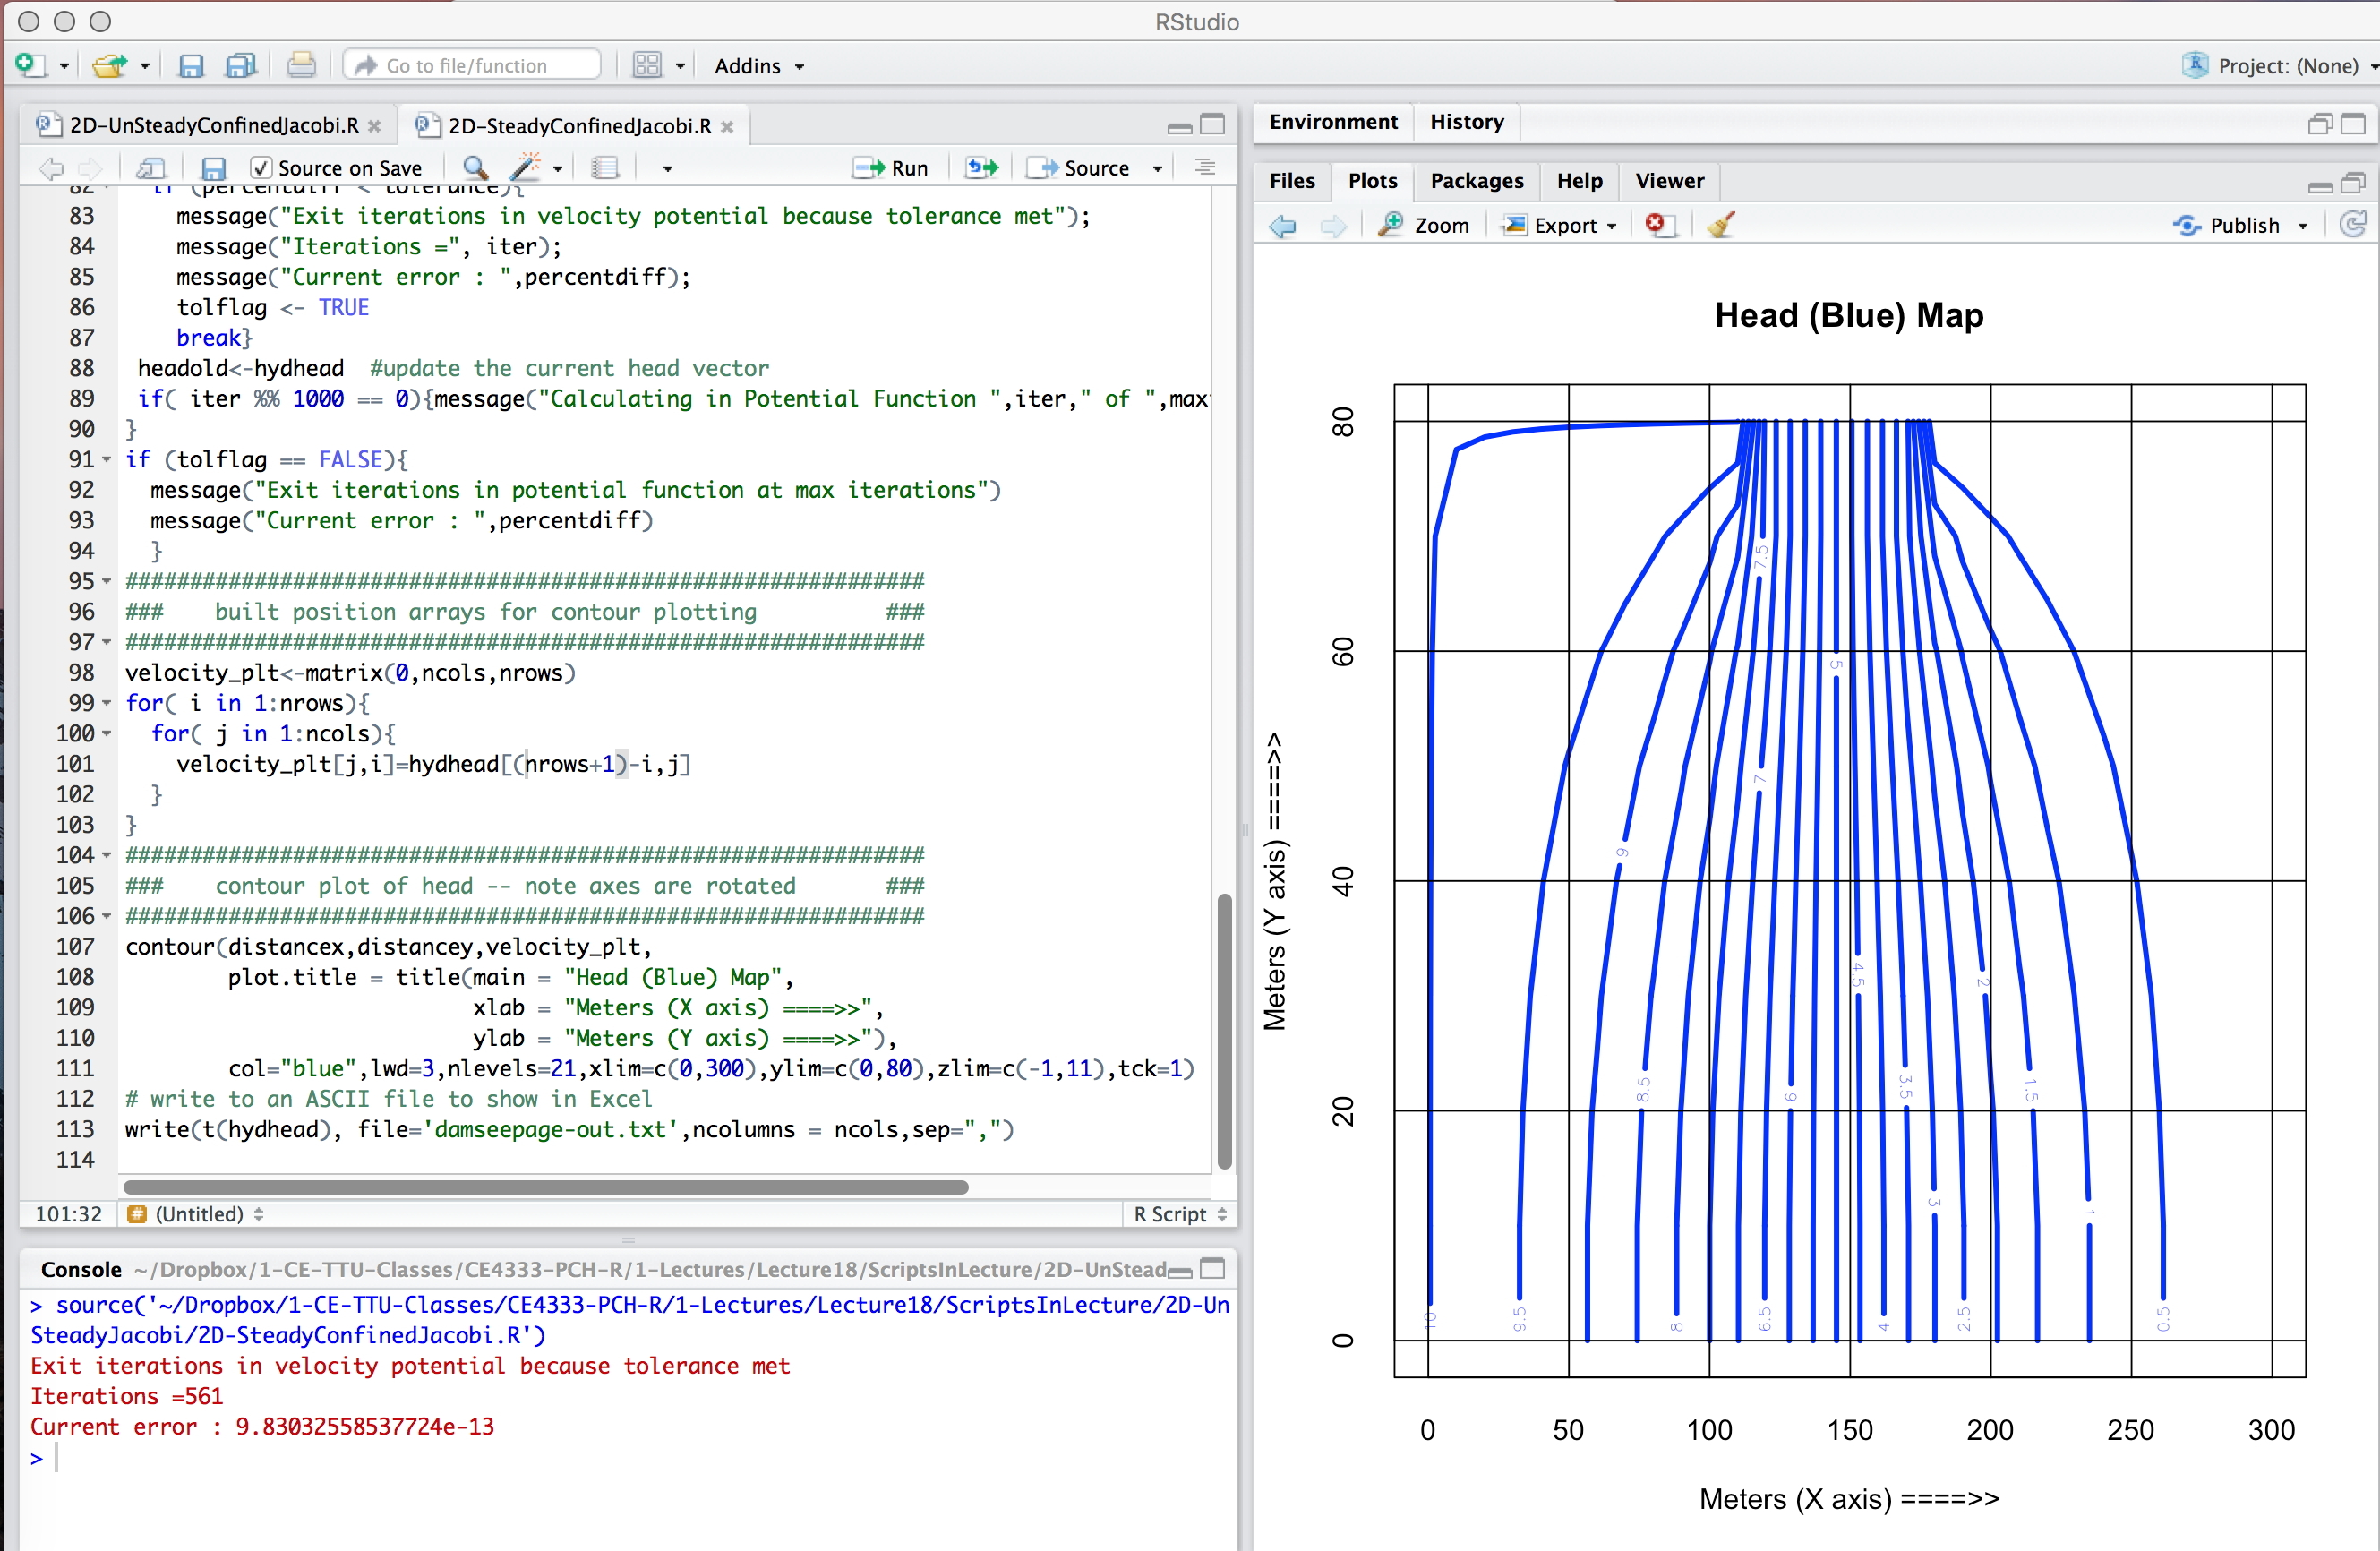
\includegraphics[width=6in]{./17-SteadyGroundwaterFlow/DamSeepageInR.jpg} 
   \caption{Screen capture of the script run with the different input file}
   \label{fig:DamSeepageInR}
\end{figure}
If we apply Darcy's law to the orange portion in the vertical direction (where flow mush be vertical to seep under the dam) the result is about 3.76 m$^3$ per day, per meter of width (perpendicular to Figure Figure \ref{fig:DamSeepage}).
These computations are shown in the spreadsheet beneath the output data.

\begin{figure}[h!] %  figure placement: here, top, bottom, or page
   \centering
   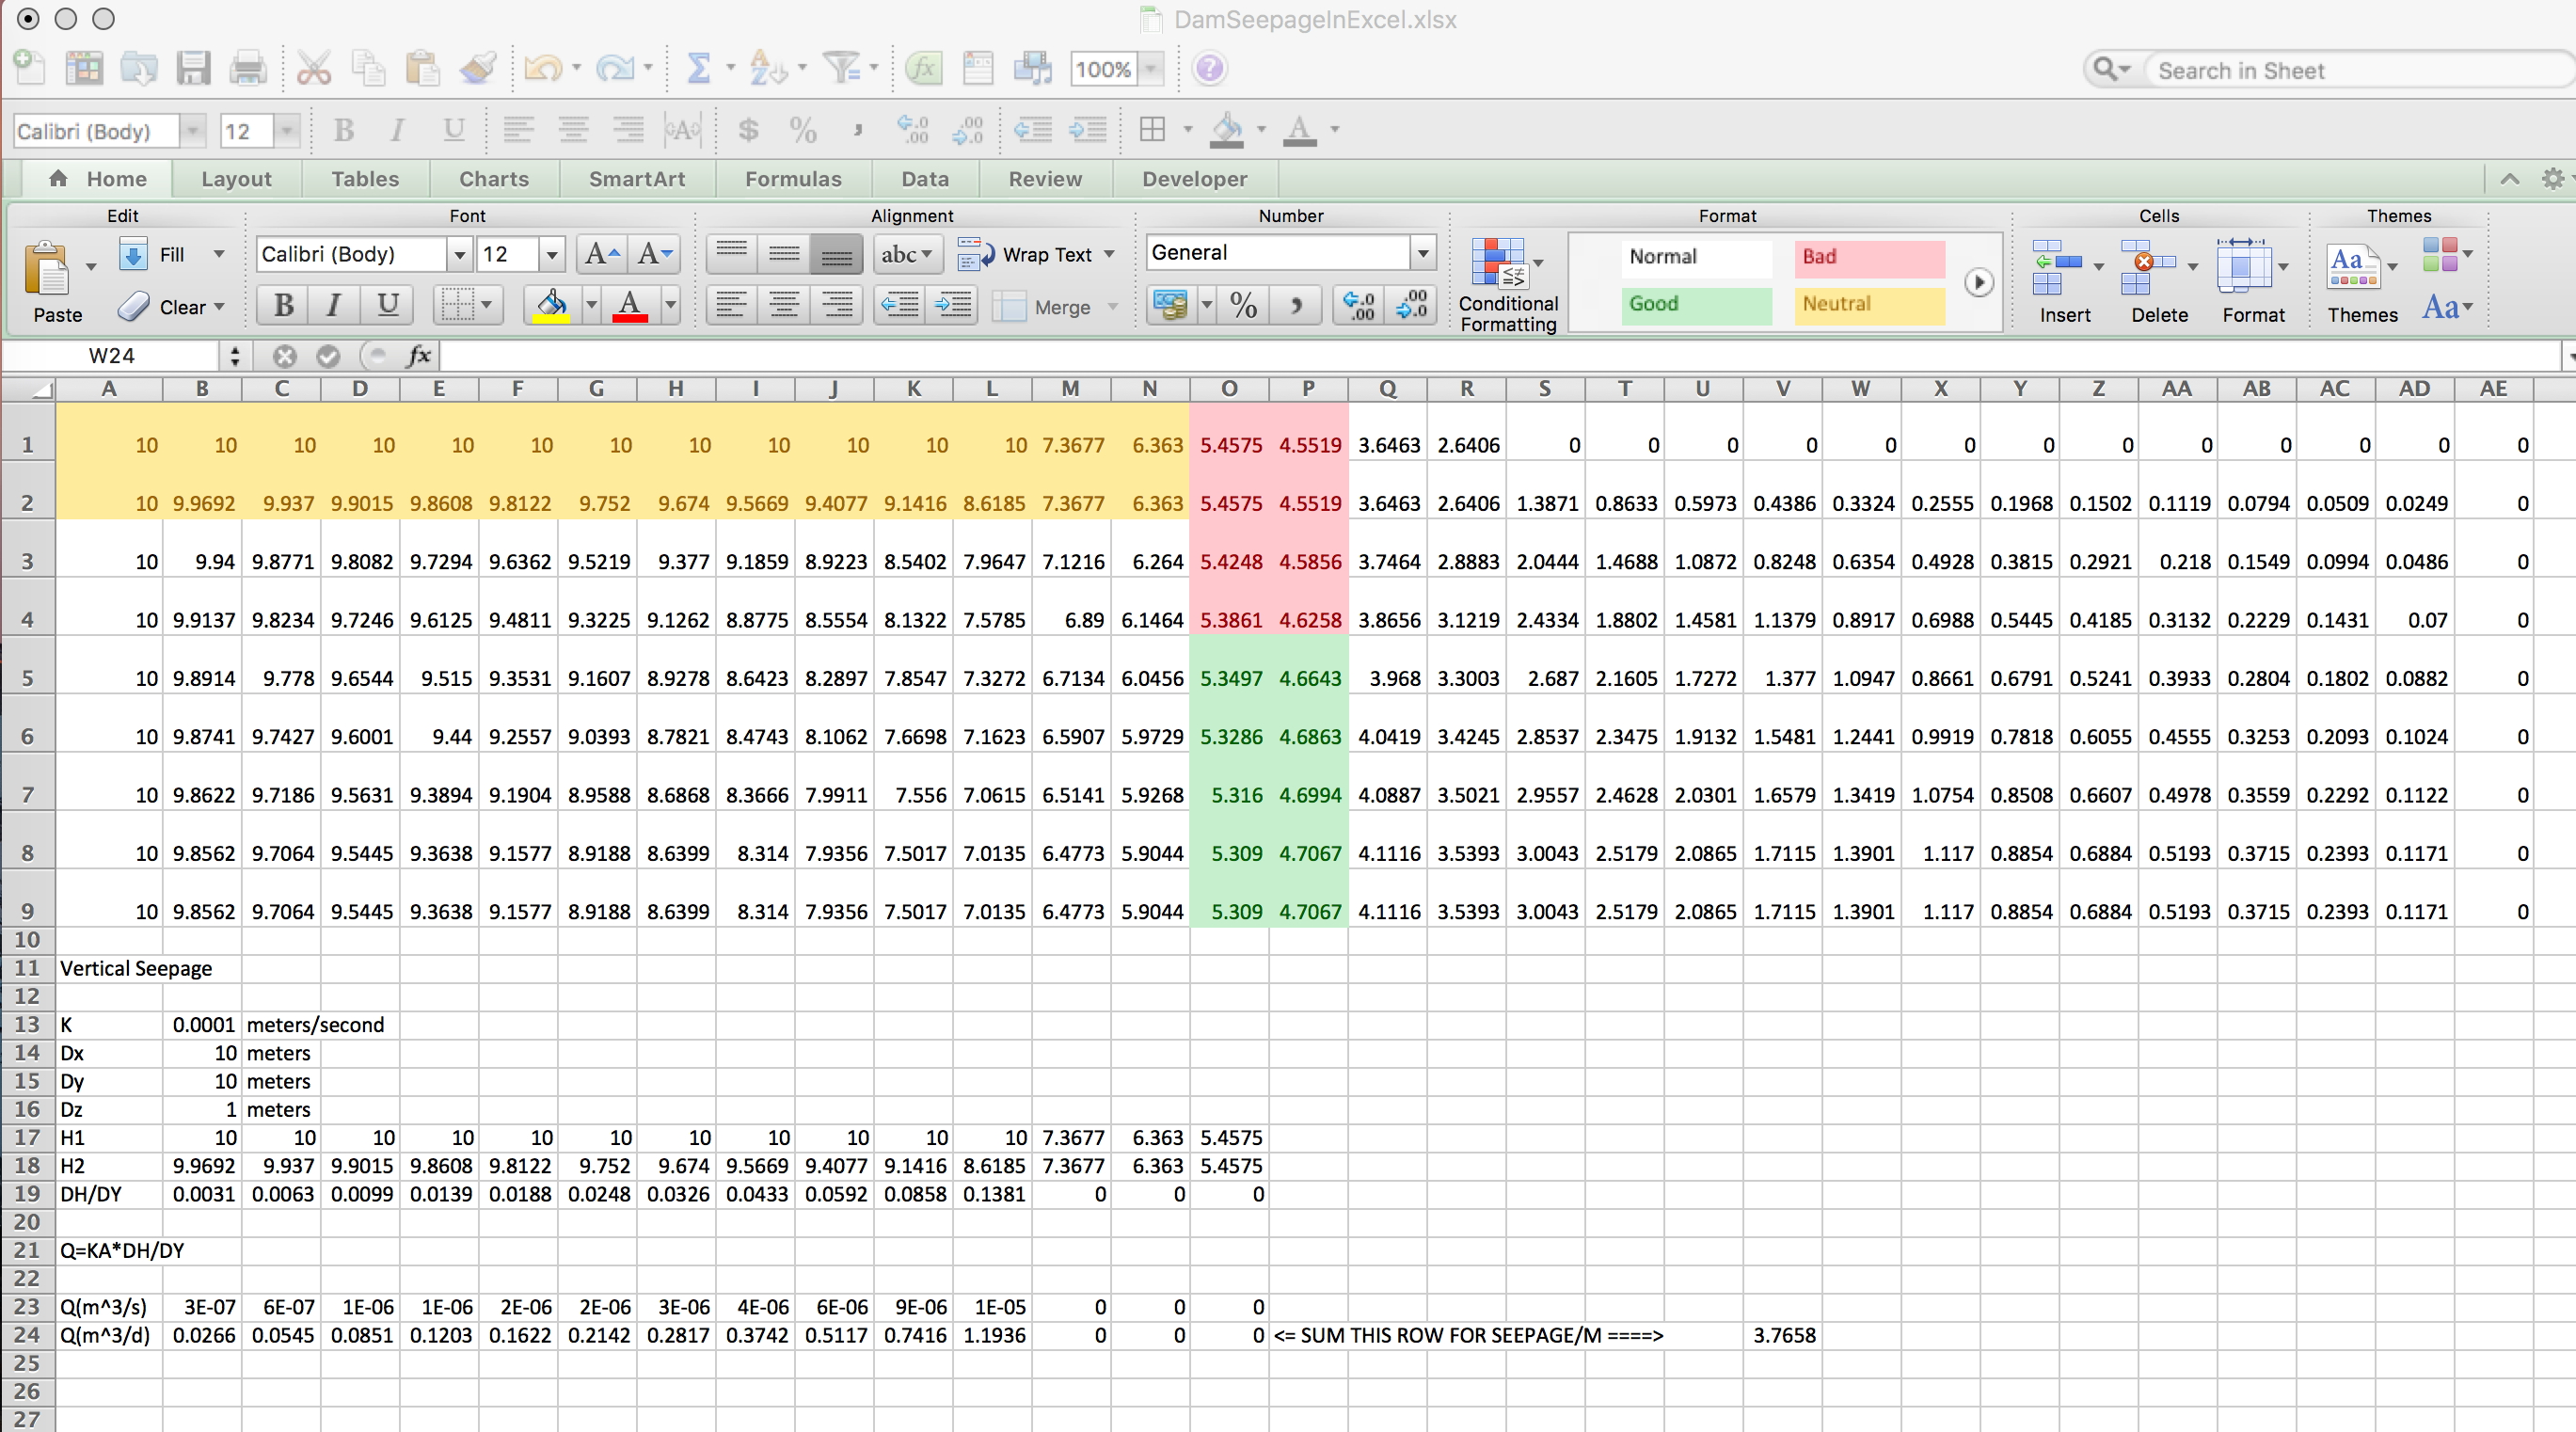
\includegraphics[width=6in]{./17-SteadyGroundwaterFlow/DamSeepageInExcel.jpg} 
   \caption{Output file loaded into Excel for further analysis}
   \label{fig:DamSeepageInExcel}
\end{figure}
\clearpage
This example (like most roll-your-own) requires some specific knowledge of hydraulics to interpret the results, in this case knowing to apply Darcy's law along the bottom of the reservoir to determine the flow rate, and to integrate (sum up) the individual cell flows to obtain total flow.

The second way to solve this example, and perhaps better is to take advantage of the symmetry and cut the domain in half, as in Figure \ref{fig:DamSeepageHalf}.  In this method we can actually specify the sheetpile as a boundary, and we will obtain the same results, but only need to supply half as much input data.

\begin{figure}[h!] %  figure placement: here, top, bottom, or page
   \centering
   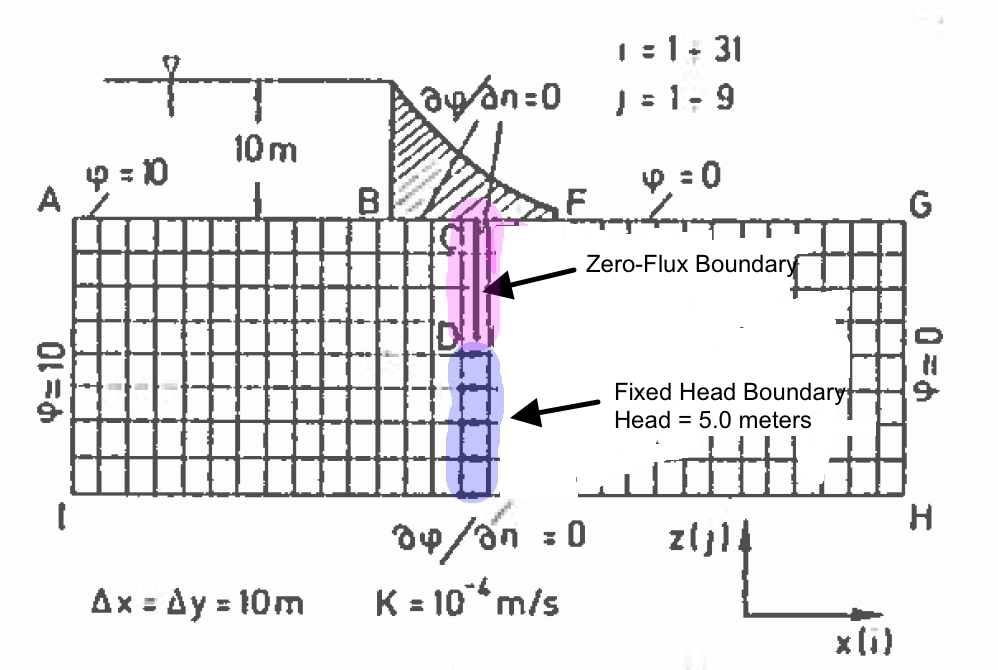
\includegraphics[width=6in]{./17-SteadyGroundwaterFlow/DamSeepageHalf.jpg} 
   \caption{Output file loaded into Excel for further analysis}
   \label{fig:DamSeepageHalf}
\end{figure}

Listing \ref{lst:DamSeepageHalf} is the input file for this symmetry based approach.

\begin{lstlisting}[caption= Input file for 2D vertical slice for Dam Seepage Example using Symmetry , label=lst:DamSeepageHalf]
10
10
1
9
15
1e-16
5000
0 10 20 30 40 50 60 70 80 90 100 110 120 130 140
0 10 20 30 40 50 60 70 80
1 1 1 1 1 1 1 1 1 1 1 1 0 0 0  
0 0 0 0 0 0 0 0 0 0 0 0 0 0 0  
1 1 1 1 1 1 1 1 1 
0 0 0 0 1 1 1 1 1 
10 10 10 10 10 10 10 10 10 10 10 10 10 10 10
10 10 10 10 10 10 10 10 10 10 10 10 10 10 10
10 10 10 10 10 10 10 10 10 10 10 10 10 10 10
10 10 10 10 10 10 10 10 10 10 10 10 10 10 10
10 10 10 10 10 10 10 10 10 10 10 10 10 10 5
10 10 10 10 10 10 10 10 10 10 10 10 10 10 5
10 10 10 10 10 10 10 10 10 10 10 10 10 10 5
10 10 10 10 10 10 10 10 10 10 10 10 10 10 5
10 10 10 10 10 10 10 10 10 10 10 10 10 10 5
0.0001 0.0001 0.0001 0.0001 0.0001 0.0001 0.0001 0.0001 0.0001 0.0001 0.0001 0.0001 0.0001 0.0001 0.0001
0.0001 0.0001 0.0001 0.0001 0.0001 0.0001 0.0001 0.0001 0.0001 0.0001 0.0001 0.0001 0.0001 0.0001 0.0001
0.0001 0.0001 0.0001 0.0001 0.0001 0.0001 0.0001 0.0001 0.0001 0.0001 0.0001 0.0001 0.0001 0.0001 0.0001
0.0001 0.0001 0.0001 0.0001 0.0001 0.0001 0.0001 0.0001 0.0001 0.0001 0.0001 0.0001 0.0001 0.0001 0.0001
0.0001 0.0001 0.0001 0.0001 0.0001 0.0001 0.0001 0.0001 0.0001 0.0001 0.0001 0.0001 0.0001 0.0001 0.0001
0.0001 0.0001 0.0001 0.0001 0.0001 0.0001 0.0001 0.0001 0.0001 0.0001 0.0001 0.0001 0.0001 0.0001 0.0001
0.0001 0.0001 0.0001 0.0001 0.0001 0.0001 0.0001 0.0001 0.0001 0.0001 0.0001 0.0001 0.0001 0.0001 0.0001
0.0001 0.0001 0.0001 0.0001 0.0001 0.0001 0.0001 0.0001 0.0001 0.0001 0.0001 0.0001 0.0001 0.0001 0.0001
0.0001 0.0001 0.0001 0.0001 0.0001 0.0001 0.0001 0.0001 0.0001 0.0001 0.0001 0.0001 0.0001 0.0001 0.0001
0.0001 0.0001 0.0001 0.0001 0.0001 0.0001 0.0001 0.0001 0.0001 0.0001 0.0001 0.0001 0.0001 0.0001 0.0001
0.0001 0.0001 0.0001 0.0001 0.0001 0.0001 0.0001 0.0001 0.0001 0.0001 0.0001 0.0001 0.0001 0.0001 0.0001
0.0001 0.0001 0.0001 0.0001 0.0001 0.0001 0.0001 0.0001 0.0001 0.0001 0.0001 0.0001 0.0001 0.0001 0.0001
0.0001 0.0001 0.0001 0.0001 0.0001 0.0001 0.0001 0.0001 0.0001 0.0001 0.0001 0.0001 0.0001 0.0001 0.0001
0.0001 0.0001 0.0001 0.0001 0.0001 0.0001 0.0001 0.0001 0.0001 0.0001 0.0001 0.0001 0.0001 0.0001 0.0001
0.0001 0.0001 0.0001 0.0001 0.0001 0.0001 0.0001 0.0001 0.0001 0.0001 0.0001 0.0001 0.0001 0.0001 0.0001
0.0001 0.0001 0.0001 0.0001 0.0001 0.0001 0.0001 0.0001 0.0001 0.0001 0.0001 0.0001 0.0001 0.0001 0.0001
0.0001 0.0001 0.0001 0.0001 0.0001 0.0001 0.0001 0.0001 0.0001 0.0001 0.0001 0.0001 0.0001 0.0001 0.0001
0.0001 0.0001 0.0001 0.0001 0.0001 0.0001 0.0001 0.0001 0.0001 0.0001 0.0001 0.0001 0.0001 0.0001 0.0001
\end{lstlisting}

Figure \ref{fig:DamSeepageHalfInR} is the result of using the half-domain approach.
\begin{figure}[h!] %  figure placement: here, top, bottom, or page
   \centering
   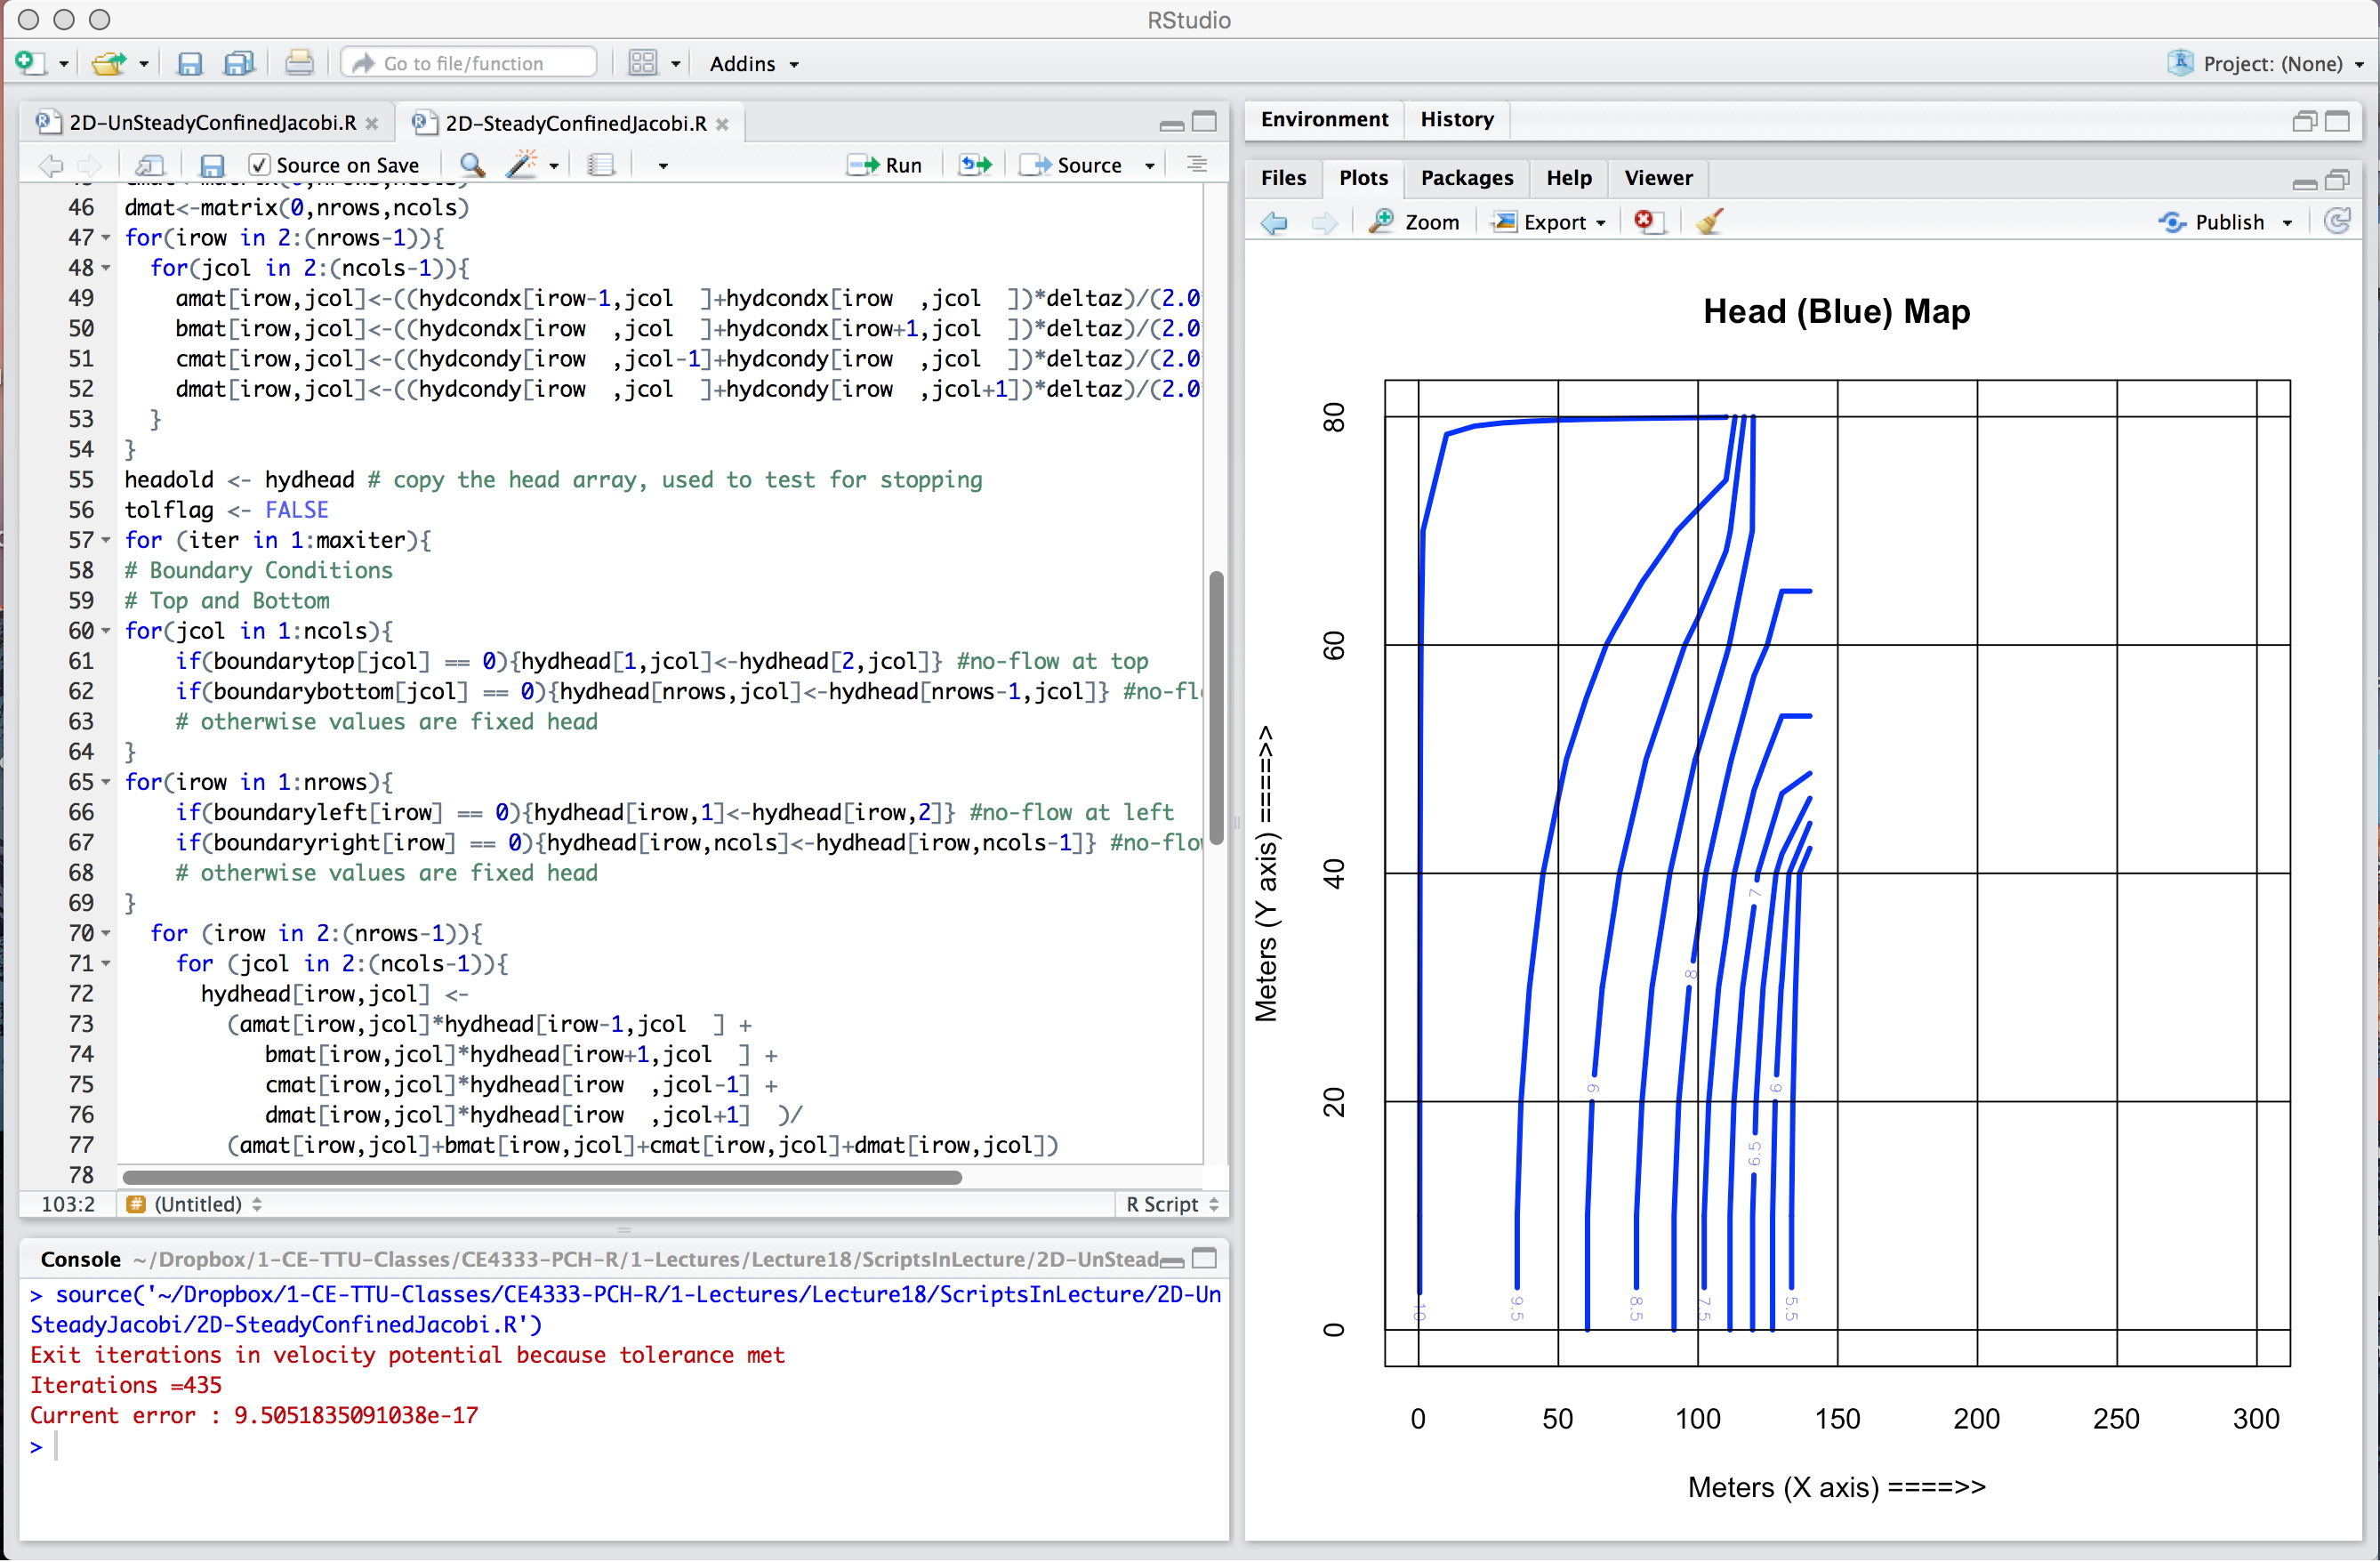
\includegraphics[width=6in]{./17-SteadyGroundwaterFlow/DamSeepageHalfInR.jpg} 
   \caption{Output file loaded into Excel for further analysis}
   \label{fig:DamSeepageHalfInR}
\end{figure}

If we repeat the flow calculations, this time along the portion at the bottom of the sheetpile, we obtain nearly the same result, 3.74 m$^3$ per day, per meter of width.  
This second way of solving the problem is more correct because we didn't have to choose an artificial value to mimic the effect of the sheetpile.

\subsubsection{Internal sources/sinks to handle a discharge (well) at a specific location}
The last concept we will add here is to illustrate a means to approximate the effect of a localized source (recharge or an injection well) or sink (pumping well).  
To incorporate these kinds of inputs we add the terms to Equation \ref{eqn:confined-aquifer-flow-PDE2D} to obtain Equation \ref{eqn:confined-aquifer-flow-PDE2D-Wells}
\begin{equation}
S \frac{\partial h}{\partial t} = 
\frac{\partial}{\partial x}({T_x \frac{\partial h}{\partial x}})
+
\frac{\partial}{\partial y}({T_y \frac{\partial h}{\partial y}})
+ R - Q
\label{eqn:confined-aquifer-flow-PDE2D-Wells}
\end{equation}
where $R$ and $Q$ are recharge and pumping expressed in dimensions of $\frac{L^3}{T}$.

The resulting difference equation is 
\begin{equation}
\begin{matrix}
0= 
[\frac{1}{\Delta x} T_{x} \frac{h_{i-1,j} - h_{i,j}}{\Delta x} +
 \frac{1}{\Delta y} T_{y} \frac{h_{i,j-1} - h_{i,j}}{\Delta y}] - \\
~~~~~~~~~~\\
~~~~~~~~~~[ \frac{1}{\Delta x} T_{x}  \frac{h_{i,j} - h_{i+1,j}}{\Delta x} +
  \frac{1}{\Delta y}  T_{y} \frac{h_{i,j} - h_{i,j+1}}{\Delta y} ]  \\
  ~~~~~~~\\
  + \frac{R_{i,j}}{\Delta x \Delta y} - \frac{Q_{i,j}}{\Delta x \Delta y} \\
\end{matrix}        
\end{equation}

These additions are incorporated into our program by only adding a few code fragments in certain places.
Listing \ref{lst:AddWellsFrags} shows the various added components to handle a well field.  
Observe we can incorporate recharge as if it were a well with a negative pumping rate so for this document it is not considered separately, although in many practical cases that might  be a preferable way to incorporate the process.

\begin{lstlisting}[caption= Input file for 2D Steady flow with generalized boundary conditions and wells , label=lst:AddWellsFrags]
# 2D Steady Confined -- With Boundary Arrays -- And Pumping Array
# 2D Aquifer Flow Model using Jacobi Iteration
# deallocate memory
rm(list=ls())
zz <- file("wellfield.dat", "r") # Open a connection named zz to file named input.dat
# read the simulation conditons
deltax <-as.numeric(readLines(zz, n = 1, ok = TRUE, warn = TRUE,encoding = "unknown", skipNul = FALSE))
deltay <-as.numeric(readLines(zz, n = 1, ok = TRUE, warn = TRUE,encoding = "unknown", skipNul = FALSE))
deltaz <-as.numeric(readLines(zz, n = 1, ok = TRUE, warn = TRUE,encoding = "unknown", skipNul = FALSE))
nrows <-as.numeric(readLines(zz, n = 1, ok = TRUE, warn = TRUE,encoding = "unknown", skipNul = FALSE))
ncols <-as.numeric(readLines(zz, n = 1, ok = TRUE, warn = TRUE,encoding = "unknown", skipNul = FALSE))
tolerance <- as.numeric(readLines(zz, n = 1, ok = TRUE, warn = TRUE,encoding = "unknown", skipNul = FALSE))
maxiter <- as.numeric(readLines(zz, n = 1, ok = TRUE, warn = TRUE,encoding = "unknown", skipNul = FALSE))
distancex <- (readLines(zz, n = 1, ok = TRUE, warn = TRUE,encoding = "unknown", skipNul = FALSE))
distancey <- (readLines(zz, n = 1, ok = TRUE, warn = TRUE,encoding = "unknown", skipNul = FALSE))
# add boundary conditions 0= fixed head, 1= no flow
boundarytop <- (readLines(zz, n = 1, ok = TRUE, warn = TRUE,encoding = "unknown", skipNul = FALSE))
boundarybottom <- (readLines(zz, n = 1, ok = TRUE, warn = TRUE,encoding = "unknown", skipNul = FALSE))
boundaryleft <- (readLines(zz, n = 1, ok = TRUE, warn = TRUE,encoding = "unknown", skipNul = FALSE))
boundaryright <- (readLines(zz, n = 1, ok = TRUE, warn = TRUE,encoding = "unknown", skipNul = FALSE))
hydhead <-(readLines(zz, n = nrows, ok = TRUE, warn = TRUE,encoding = "unknown", skipNul = FALSE))
# hydhead is now the initial condition array #
hydcondx <-(readLines(zz, n = nrows, ok = TRUE, warn = TRUE,encoding = "unknown", skipNul = FALSE))
hydcondy <-(readLines(zz, n = nrows, ok = TRUE, warn = TRUE,encoding = "unknown", skipNul = FALSE))
# add pumping array
pumping <-(readLines(zz, n = nrows, ok = TRUE, warn = TRUE,encoding = "unknown", skipNul = FALSE))
close(zz)
# split the multiple column strings into numeric components for a vector
distancex <-as.numeric(unlist(strsplit(distancex,split=" ")))
distancey <-as.numeric(unlist(strsplit(distancey,split=" ")))
boundarytop <-as.numeric(unlist(strsplit(boundarytop,split=" ")))
boundarybottom <-as.numeric(unlist(strsplit(boundarybottom,split=" ")))
boundaryleft <-as.numeric(unlist(strsplit(boundaryleft,split=" ")))
boundaryright <-as.numeric(unlist(strsplit(boundaryright,split=" ")))
hydhead <-as.numeric(unlist(strsplit(hydhead,split=" ")))
hydcondx <-as.numeric(unlist(strsplit(hydcondx,split=" ")))
hydcondy <-as.numeric(unlist(strsplit(hydcondy,split=" ")))
pumping <-as.numeric(unlist(strsplit(pumping,split=" ")))
# convert the numeric vectors into matrices for easier indexing
hydhead <- matrix(hydhead,nrow=nrows,ncol=ncols,byrow = TRUE)
hydcondx <-matrix(hydcondx,nrow=nrows,ncol=ncols,byrow = TRUE)
hydcondy <-matrix(hydcondy,nrow=nrows,ncol=ncols,byrow = TRUE)
pumping <-matrix(pumping,nrow=nrows,ncol=ncols,byrow = TRUE)
# here we perform the velocity potential calculations
# built the transmissivity arrays
amat<-matrix(0,nrows,ncols) 
bmat<-matrix(0,nrows,ncols) 
cmat<-matrix(0,nrows,ncols)
dmat<-matrix(0,nrows,ncols)
qrat<-matrix(0,nrows,ncols)
for(irow in 2:(nrows-1)){
  for(jcol in 2:(ncols-1)){
    amat[irow,jcol]<-((hydcondx[irow-1,jcol  ]+hydcondx[irow  ,jcol  ])*deltaz)/(2.0*deltax^2)
    bmat[irow,jcol]<-((hydcondx[irow  ,jcol  ]+hydcondx[irow+1,jcol  ])*deltaz)/(2.0*deltax^2)
    cmat[irow,jcol]<-((hydcondy[irow  ,jcol-1]+hydcondy[irow  ,jcol  ])*deltaz)/(2.0*deltay^2)
    dmat[irow,jcol]<-((hydcondy[irow  ,jcol  ]+hydcondy[irow  ,jcol+1])*deltaz)/(2.0*deltay^2)
    qrat[irow,jcol]<-(-1.0)*pumping[irow,jcol]/(deltax*deltay)
  }
}
headold <- hydhead # copy the head array, used to test for stopping 
tolflag <- FALSE
for (iter in 1:maxiter){
# Boundary Conditions
# Top and Bottom
for(jcol in 1:ncols){
    if(boundarytop[jcol] == 0){hydhead[1,jcol]<-hydhead[2,jcol]} #no-flow at top
    if(boundarybottom[jcol] == 0){hydhead[nrows,jcol]<-hydhead[nrows-1,jcol]} #no-flow at bottom
    # otherwise values are fixed head
}
for(irow in 1:nrows){
    if(boundaryleft[irow] == 0){hydhead[irow,1]<-hydhead[irow,2]} #no-flow at left
    if(boundaryright[irow] == 0){hydhead[irow,ncols]<-hydhead[irow,ncols-1]} #no-flow at right
    # otherwise values are fixed head
}
  for (irow in 2:(nrows-1)){
    for (jcol in 2:(ncols-1)){
      hydhead[irow,jcol] <- 
          (                       qrat[irow,jcol] +
           amat[irow,jcol]*hydhead[irow-1,jcol  ] +
           bmat[irow,jcol]*hydhead[irow+1,jcol  ] +
           cmat[irow,jcol]*hydhead[irow  ,jcol-1] +
           dmat[irow,jcol]*hydhead[irow  ,jcol+1]  )/
        (amat[irow,jcol]+bmat[irow,jcol]+cmat[irow,jcol]+dmat[irow,jcol])
    }
  }
  # test for stopping iterations
  percentdiff <- sum((hydhead-headold)^2)
  if (percentdiff < tolerance){
    message("Exit iterations in velocity potential because tolerance met");
    message("Iterations =", iter);
    message("Current error : ",percentdiff);
    tolflag <- TRUE
    break}
 headold<-hydhead  #update the current head vector
 if( iter %% 1000 == 0){message("Calculating in Potential Function ",iter," of ",maxiter, " iterations")}
}
if (tolflag == FALSE){
  message("Exit iterations in potential function at max iterations")
  message("Current error : ",percentdiff)
  }
##############################################################
###    built position arrays for contour plotting          ###
##############################################################
velocity_plt<-matrix(0,ncols,nrows) 
for( i in 1:nrows){
  for( j in 1:ncols){
    velocity_plt[j,i]=hydhead[(nrows+1)-i,j]
  }
}
##############################################################
###    contour plot of head -- note axes are rotated       ###
##############################################################
contour(distancex,distancey,velocity_plt,
        plot.title = title(main = "Head (Blue) Map",
                           xlab = "Meters (X axis) ====>>", 
                           ylab = "Meters (Y axis) ====>>"),
        col="blue",lwd=3,nlevels=21,xlim=c(0,300),ylim=c(0,300),zlim=c(-1,40),tck=1)
# write to an ASCII file to show in Excel
write(t(hydhead), file='damseepage-out.txt',ncolumns = ncols,sep=",") 
message("min head : ",min(hydhead))
\end{lstlisting}


\textbf{Example 5: 4 Wells in a rectangular aquifer}
Figure \ref{fig:4WellsSteady} is a rectangular aquifer with 4 wells as shown.
The aquifer thickness is 1 meters.
The aquifer is surrounded with a constant head boundary of 30 meters.
The hydraulic conductivity is $K=0.033~m/day$.

Using a $10~meter~\times~10~meter$ grid spacing estimate the pumping rate in each well so that the head within the rectangular area defined by the well field is no greater than 15 meters.
\begin{figure}[h!] %  figure placement: here, top, bottom, or page
   \centering
   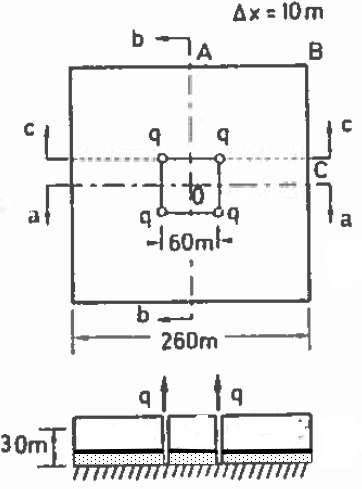
\includegraphics[height=4in]{./17-SteadyGroundwaterFlow/4WellsSteady.jpg} 
   \caption{Rectangular aquifer with 4 wells}
   \label{fig:4WellsSteady}
\end{figure}
\clearpage

Listing \ref{lst:wellfield} is the input file for the modified script for the example problem.  
The file takes several pages in this document --- as the input requirements become substantial, one would write separate scripts just to build input files to structure them properly.  
We are essentially constructing a specialized database, and manually building that database can become tedious whereas we can automatically populate portions of the database with a script. 

\begin{lstlisting}[caption= Input file for 4 well example , label=lst:wellfield]
10
10
1
28
28
1e-16
5000
0 10 20 30 40 50 60 70 80 90 100 110 120 130 140 150 160 170 180 190 200 210 220 230 240 250 260 270
0 10 20 30 40 50 60 70 80 90 100 110 120 130 140 150 160 170 180 190 200 210 220 230 240 250 260 270
1 1 1 1 1 1 1 1 1 1 1 1 1 1 1 1 1 1 1 1 1 1 1 1 1 1 1 1 
1 1 1 1 1 1 1 1 1 1 1 1 1 1 1 1 1 1 1 1 1 1 1 1 1 1 1 1
1 1 1 1 1 1 1 1 1 1 1 1 1 1 1 1 1 1 1 1 1 1 1 1 1 1 1 1
1 1 1 1 1 1 1 1 1 1 1 1 1 1 1 1 1 1 1 1 1 1 1 1 1 1 1 1 
30 30 30 30 30 30 30 30 30 30 30 30 30 30 30 30 30 30 30 30 30 30 30 30 30 30 30 30
30 30 30 30 30 30 30 30 30 30 30 30 30 30 30 30 30 30 30 30 30 30 30 30 30 30 30 30
30 30 30 30 30 30 30 30 30 30 30 30 30 30 30 30 30 30 30 30 30 30 30 30 30 30 30 30
30 30 30 30 30 30 30 30 30 30 30 30 30 30 30 30 30 30 30 30 30 30 30 30 30 30 30 30
30 30 30 30 30 30 30 30 30 30 30 30 30 30 30 30 30 30 30 30 30 30 30 30 30 30 30 30
30 30 30 30 30 30 30 30 30 30 30 30 30 30 30 30 30 30 30 30 30 30 30 30 30 30 30 30
30 30 30 30 30 30 30 30 30 30 30 30 30 30 30 30 30 30 30 30 30 30 30 30 30 30 30 30
30 30 30 30 30 30 30 30 30 30 30 30 30 30 30 30 30 30 30 30 30 30 30 30 30 30 30 30
30 30 30 30 30 30 30 30 30 30 30 30 30 30 30 30 30 30 30 30 30 30 30 30 30 30 30 30
30 30 30 30 30 30 30 30 30 30 30 30 30 30 30 30 30 30 30 30 30 30 30 30 30 30 30 30
30 30 30 30 30 30 30 30 30 30 30 30 30 30 30 30 30 30 30 30 30 30 30 30 30 30 30 30
30 30 30 30 30 30 30 30 30 30 30 30 30 30 30 30 30 30 30 30 30 30 30 30 30 30 30 30
30 30 30 30 30 30 30 30 30 30 30 30 30 30 30 30 30 30 30 30 30 30 30 30 30 30 30 30
30 30 30 30 30 30 30 30 30 30 30 30 30 30 30 30 30 30 30 30 30 30 30 30 30 30 30 30
30 30 30 30 30 30 30 30 30 30 30 30 30 30 30 30 30 30 30 30 30 30 30 30 30 30 30 30
30 30 30 30 30 30 30 30 30 30 30 30 30 30 30 30 30 30 30 30 30 30 30 30 30 30 30 30
30 30 30 30 30 30 30 30 30 30 30 30 30 30 30 30 30 30 30 30 30 30 30 30 30 30 30 30
30 30 30 30 30 30 30 30 30 30 30 30 30 30 30 30 30 30 30 30 30 30 30 30 30 30 30 30
30 30 30 30 30 30 30 30 30 30 30 30 30 30 30 30 30 30 30 30 30 30 30 30 30 30 30 30
30 30 30 30 30 30 30 30 30 30 30 30 30 30 30 30 30 30 30 30 30 30 30 30 30 30 30 30
30 30 30 30 30 30 30 30 30 30 30 30 30 30 30 30 30 30 30 30 30 30 30 30 30 30 30 30
30 30 30 30 30 30 30 30 30 30 30 30 30 30 30 30 30 30 30 30 30 30 30 30 30 30 30 30
30 30 30 30 30 30 30 30 30 30 30 30 30 30 30 30 30 30 30 30 30 30 30 30 30 30 30 30
30 30 30 30 30 30 30 30 30 30 30 30 30 30 30 30 30 30 30 30 30 30 30 30 30 30 30 30
30 30 30 30 30 30 30 30 30 30 30 30 30 30 30 30 30 30 30 30 30 30 30 30 30 30 30 30
30 30 30 30 30 30 30 30 30 30 30 30 30 30 30 30 30 30 30 30 30 30 30 30 30 30 30 30
30 30 30 30 30 30 30 30 30 30 30 30 30 30 30 30 30 30 30 30 30 30 30 30 30 30 30 30
30 30 30 30 30 30 30 30 30 30 30 30 30 30 30 30 30 30 30 30 30 30 30 30 30 30 30 30
0.033 0.033 0.033 0.033 0.033 0.033 0.033 0.033 0.033 0.033 0.033 0.033 0.033 0.033 0.033 0.033 0.033 0.033 0.033 0.033 0.033 0.033 0.033 0.033 0.033 0.033 0.033 0.033
0.033 0.033 0.033 0.033 0.033 0.033 0.033 0.033 0.033 0.033 0.033 0.033 0.033 0.033 0.033 0.033 0.033 0.033 0.033 0.033 0.033 0.033 0.033 0.033 0.033 0.033 0.033 0.033
0.033 0.033 0.033 0.033 0.033 0.033 0.033 0.033 0.033 0.033 0.033 0.033 0.033 0.033 0.033 0.033 0.033 0.033 0.033 0.033 0.033 0.033 0.033 0.033 0.033 0.033 0.033 0.033
0.033 0.033 0.033 0.033 0.033 0.033 0.033 0.033 0.033 0.033 0.033 0.033 0.033 0.033 0.033 0.033 0.033 0.033 0.033 0.033 0.033 0.033 0.033 0.033 0.033 0.033 0.033 0.033
0.033 0.033 0.033 0.033 0.033 0.033 0.033 0.033 0.033 0.033 0.033 0.033 0.033 0.033 0.033 0.033 0.033 0.033 0.033 0.033 0.033 0.033 0.033 0.033 0.033 0.033 0.033 0.033
0.033 0.033 0.033 0.033 0.033 0.033 0.033 0.033 0.033 0.033 0.033 0.033 0.033 0.033 0.033 0.033 0.033 0.033 0.033 0.033 0.033 0.033 0.033 0.033 0.033 0.033 0.033 0.033
0.033 0.033 0.033 0.033 0.033 0.033 0.033 0.033 0.033 0.033 0.033 0.033 0.033 0.033 0.033 0.033 0.033 0.033 0.033 0.033 0.033 0.033 0.033 0.033 0.033 0.033 0.033 0.033
0.033 0.033 0.033 0.033 0.033 0.033 0.033 0.033 0.033 0.033 0.033 0.033 0.033 0.033 0.033 0.033 0.033 0.033 0.033 0.033 0.033 0.033 0.033 0.033 0.033 0.033 0.033 0.033
0.033 0.033 0.033 0.033 0.033 0.033 0.033 0.033 0.033 0.033 0.033 0.033 0.033 0.033 0.033 0.033 0.033 0.033 0.033 0.033 0.033 0.033 0.033 0.033 0.033 0.033 0.033 0.033
0.033 0.033 0.033 0.033 0.033 0.033 0.033 0.033 0.033 0.033 0.033 0.033 0.033 0.033 0.033 0.033 0.033 0.033 0.033 0.033 0.033 0.033 0.033 0.033 0.033 0.033 0.033 0.033
0.033 0.033 0.033 0.033 0.033 0.033 0.033 0.033 0.033 0.033 0.033 0.033 0.033 0.033 0.033 0.033 0.033 0.033 0.033 0.033 0.033 0.033 0.033 0.033 0.033 0.033 0.033 0.033
0.033 0.033 0.033 0.033 0.033 0.033 0.033 0.033 0.033 0.033 0.033 0.033 0.033 0.033 0.033 0.033 0.033 0.033 0.033 0.033 0.033 0.033 0.033 0.033 0.033 0.033 0.033 0.033
0.033 0.033 0.033 0.033 0.033 0.033 0.033 0.033 0.033 0.033 0.033 0.033 0.033 0.033 0.033 0.033 0.033 0.033 0.033 0.033 0.033 0.033 0.033 0.033 0.033 0.033 0.033 0.033
0.033 0.033 0.033 0.033 0.033 0.033 0.033 0.033 0.033 0.033 0.033 0.033 0.033 0.033 0.033 0.033 0.033 0.033 0.033 0.033 0.033 0.033 0.033 0.033 0.033 0.033 0.033 0.033
0.033 0.033 0.033 0.033 0.033 0.033 0.033 0.033 0.033 0.033 0.033 0.033 0.033 0.033 0.033 0.033 0.033 0.033 0.033 0.033 0.033 0.033 0.033 0.033 0.033 0.033 0.033 0.033
0.033 0.033 0.033 0.033 0.033 0.033 0.033 0.033 0.033 0.033 0.033 0.033 0.033 0.033 0.033 0.033 0.033 0.033 0.033 0.033 0.033 0.033 0.033 0.033 0.033 0.033 0.033 0.033
0.033 0.033 0.033 0.033 0.033 0.033 0.033 0.033 0.033 0.033 0.033 0.033 0.033 0.033 0.033 0.033 0.033 0.033 0.033 0.033 0.033 0.033 0.033 0.033 0.033 0.033 0.033 0.033
0.033 0.033 0.033 0.033 0.033 0.033 0.033 0.033 0.033 0.033 0.033 0.033 0.033 0.033 0.033 0.033 0.033 0.033 0.033 0.033 0.033 0.033 0.033 0.033 0.033 0.033 0.033 0.033
0.033 0.033 0.033 0.033 0.033 0.033 0.033 0.033 0.033 0.033 0.033 0.033 0.033 0.033 0.033 0.033 0.033 0.033 0.033 0.033 0.033 0.033 0.033 0.033 0.033 0.033 0.033 0.033
0.033 0.033 0.033 0.033 0.033 0.033 0.033 0.033 0.033 0.033 0.033 0.033 0.033 0.033 0.033 0.033 0.033 0.033 0.033 0.033 0.033 0.033 0.033 0.033 0.033 0.033 0.033 0.033
0.033 0.033 0.033 0.033 0.033 0.033 0.033 0.033 0.033 0.033 0.033 0.033 0.033 0.033 0.033 0.033 0.033 0.033 0.033 0.033 0.033 0.033 0.033 0.033 0.033 0.033 0.033 0.033
0.033 0.033 0.033 0.033 0.033 0.033 0.033 0.033 0.033 0.033 0.033 0.033 0.033 0.033 0.033 0.033 0.033 0.033 0.033 0.033 0.033 0.033 0.033 0.033 0.033 0.033 0.033 0.033
0.033 0.033 0.033 0.033 0.033 0.033 0.033 0.033 0.033 0.033 0.033 0.033 0.033 0.033 0.033 0.033 0.033 0.033 0.033 0.033 0.033 0.033 0.033 0.033 0.033 0.033 0.033 0.033
0.033 0.033 0.033 0.033 0.033 0.033 0.033 0.033 0.033 0.033 0.033 0.033 0.033 0.033 0.033 0.033 0.033 0.033 0.033 0.033 0.033 0.033 0.033 0.033 0.033 0.033 0.033 0.033
0.033 0.033 0.033 0.033 0.033 0.033 0.033 0.033 0.033 0.033 0.033 0.033 0.033 0.033 0.033 0.033 0.033 0.033 0.033 0.033 0.033 0.033 0.033 0.033 0.033 0.033 0.033 0.033
0.033 0.033 0.033 0.033 0.033 0.033 0.033 0.033 0.033 0.033 0.033 0.033 0.033 0.033 0.033 0.033 0.033 0.033 0.033 0.033 0.033 0.033 0.033 0.033 0.033 0.033 0.033 0.033
0.033 0.033 0.033 0.033 0.033 0.033 0.033 0.033 0.033 0.033 0.033 0.033 0.033 0.033 0.033 0.033 0.033 0.033 0.033 0.033 0.033 0.033 0.033 0.033 0.033 0.033 0.033 0.033
0.033 0.033 0.033 0.033 0.033 0.033 0.033 0.033 0.033 0.033 0.033 0.033 0.033 0.033 0.033 0.033 0.033 0.033 0.033 0.033 0.033 0.033 0.033 0.033 0.033 0.033 0.033 0.033
0.033 0.033 0.033 0.033 0.033 0.033 0.033 0.033 0.033 0.033 0.033 0.033 0.033 0.033 0.033 0.033 0.033 0.033 0.033 0.033 0.033 0.033 0.033 0.033 0.033 0.033 0.033 0.033
0.033 0.033 0.033 0.033 0.033 0.033 0.033 0.033 0.033 0.033 0.033 0.033 0.033 0.033 0.033 0.033 0.033 0.033 0.033 0.033 0.033 0.033 0.033 0.033 0.033 0.033 0.033 0.033
0.033 0.033 0.033 0.033 0.033 0.033 0.033 0.033 0.033 0.033 0.033 0.033 0.033 0.033 0.033 0.033 0.033 0.033 0.033 0.033 0.033 0.033 0.033 0.033 0.033 0.033 0.033 0.033
0.033 0.033 0.033 0.033 0.033 0.033 0.033 0.033 0.033 0.033 0.033 0.033 0.033 0.033 0.033 0.033 0.033 0.033 0.033 0.033 0.033 0.033 0.033 0.033 0.033 0.033 0.033 0.033
0.033 0.033 0.033 0.033 0.033 0.033 0.033 0.033 0.033 0.033 0.033 0.033 0.033 0.033 0.033 0.033 0.033 0.033 0.033 0.033 0.033 0.033 0.033 0.033 0.033 0.033 0.033 0.033
0.033 0.033 0.033 0.033 0.033 0.033 0.033 0.033 0.033 0.033 0.033 0.033 0.033 0.033 0.033 0.033 0.033 0.033 0.033 0.033 0.033 0.033 0.033 0.033 0.033 0.033 0.033 0.033
0.033 0.033 0.033 0.033 0.033 0.033 0.033 0.033 0.033 0.033 0.033 0.033 0.033 0.033 0.033 0.033 0.033 0.033 0.033 0.033 0.033 0.033 0.033 0.033 0.033 0.033 0.033 0.033
0.033 0.033 0.033 0.033 0.033 0.033 0.033 0.033 0.033 0.033 0.033 0.033 0.033 0.033 0.033 0.033 0.033 0.033 0.033 0.033 0.033 0.033 0.033 0.033 0.033 0.033 0.033 0.033
0.033 0.033 0.033 0.033 0.033 0.033 0.033 0.033 0.033 0.033 0.033 0.033 0.033 0.033 0.033 0.033 0.033 0.033 0.033 0.033 0.033 0.033 0.033 0.033 0.033 0.033 0.033 0.033
0.033 0.033 0.033 0.033 0.033 0.033 0.033 0.033 0.033 0.033 0.033 0.033 0.033 0.033 0.033 0.033 0.033 0.033 0.033 0.033 0.033 0.033 0.033 0.033 0.033 0.033 0.033 0.033
0.033 0.033 0.033 0.033 0.033 0.033 0.033 0.033 0.033 0.033 0.033 0.033 0.033 0.033 0.033 0.033 0.033 0.033 0.033 0.033 0.033 0.033 0.033 0.033 0.033 0.033 0.033 0.033
0.033 0.033 0.033 0.033 0.033 0.033 0.033 0.033 0.033 0.033 0.033 0.033 0.033 0.033 0.033 0.033 0.033 0.033 0.033 0.033 0.033 0.033 0.033 0.033 0.033 0.033 0.033 0.033
0.033 0.033 0.033 0.033 0.033 0.033 0.033 0.033 0.033 0.033 0.033 0.033 0.033 0.033 0.033 0.033 0.033 0.033 0.033 0.033 0.033 0.033 0.033 0.033 0.033 0.033 0.033 0.033
0.033 0.033 0.033 0.033 0.033 0.033 0.033 0.033 0.033 0.033 0.033 0.033 0.033 0.033 0.033 0.033 0.033 0.033 0.033 0.033 0.033 0.033 0.033 0.033 0.033 0.033 0.033 0.033
0.033 0.033 0.033 0.033 0.033 0.033 0.033 0.033 0.033 0.033 0.033 0.033 0.033 0.033 0.033 0.033 0.033 0.033 0.033 0.033 0.033 0.033 0.033 0.033 0.033 0.033 0.033 0.033
0.033 0.033 0.033 0.033 0.033 0.033 0.033 0.033 0.033 0.033 0.033 0.033 0.033 0.033 0.033 0.033 0.033 0.033 0.033 0.033 0.033 0.033 0.033 0.033 0.033 0.033 0.033 0.033
0.033 0.033 0.033 0.033 0.033 0.033 0.033 0.033 0.033 0.033 0.033 0.033 0.033 0.033 0.033 0.033 0.033 0.033 0.033 0.033 0.033 0.033 0.033 0.033 0.033 0.033 0.033 0.033
0.033 0.033 0.033 0.033 0.033 0.033 0.033 0.033 0.033 0.033 0.033 0.033 0.033 0.033 0.033 0.033 0.033 0.033 0.033 0.033 0.033 0.033 0.033 0.033 0.033 0.033 0.033 0.033
0.033 0.033 0.033 0.033 0.033 0.033 0.033 0.033 0.033 0.033 0.033 0.033 0.033 0.033 0.033 0.033 0.033 0.033 0.033 0.033 0.033 0.033 0.033 0.033 0.033 0.033 0.033 0.033
0.033 0.033 0.033 0.033 0.033 0.033 0.033 0.033 0.033 0.033 0.033 0.033 0.033 0.033 0.033 0.033 0.033 0.033 0.033 0.033 0.033 0.033 0.033 0.033 0.033 0.033 0.033 0.033
0.033 0.033 0.033 0.033 0.033 0.033 0.033 0.033 0.033 0.033 0.033 0.033 0.033 0.033 0.033 0.033 0.033 0.033 0.033 0.033 0.033 0.033 0.033 0.033 0.033 0.033 0.033 0.033
0.033 0.033 0.033 0.033 0.033 0.033 0.033 0.033 0.033 0.033 0.033 0.033 0.033 0.033 0.033 0.033 0.033 0.033 0.033 0.033 0.033 0.033 0.033 0.033 0.033 0.033 0.033 0.033
0.033 0.033 0.033 0.033 0.033 0.033 0.033 0.033 0.033 0.033 0.033 0.033 0.033 0.033 0.033 0.033 0.033 0.033 0.033 0.033 0.033 0.033 0.033 0.033 0.033 0.033 0.033 0.033
0.033 0.033 0.033 0.033 0.033 0.033 0.033 0.033 0.033 0.033 0.033 0.033 0.033 0.033 0.033 0.033 0.033 0.033 0.033 0.033 0.033 0.033 0.033 0.033 0.033 0.033 0.033 0.033
0.033 0.033 0.033 0.033 0.033 0.033 0.033 0.033 0.033 0.033 0.033 0.033 0.033 0.033 0.033 0.033 0.033 0.033 0.033 0.033 0.033 0.033 0.033 0.033 0.033 0.033 0.033 0.033
0.033 0.033 0.033 0.033 0.033 0.033 0.033 0.033 0.033 0.033 0.033 0.033 0.033 0.033 0.033 0.033 0.033 0.033 0.033 0.033 0.033 0.033 0.033 0.033 0.033 0.033 0.033 0.033
0.033 0.033 0.033 0.033 0.033 0.033 0.033 0.033 0.033 0.033 0.033 0.033 0.033 0.033 0.033 0.033 0.033 0.033 0.033 0.033 0.033 0.033 0.033 0.033 0.033 0.033 0.033 0.033
0.033 0.033 0.033 0.033 0.033 0.033 0.033 0.033 0.033 0.033 0.033 0.033 0.033 0.033 0.033 0.033 0.033 0.033 0.033 0.033 0.033 0.033 0.033 0.033 0.033 0.033 0.033 0.033
0.000 0.000 0.000 0.000 0.000 0.000 0.000 0.000 0.000 0.000 0.000 0.000 0.000 0.000 0.000 0.000 0.000 0.000 0.000 0.000 0.000 0.000 0.000 0.000 0.000 0.000 0.000 0.000
0.000 0.000 0.000 0.000 0.000 0.000 0.000 0.000 0.000 0.000 0.000 0.000 0.000 0.000 0.000 0.000 0.000 0.000 0.000 0.000 0.000 0.000 0.000 0.000 0.000 0.000 0.000 0.000
0.000 0.000 0.000 0.000 0.000 0.000 0.000 0.000 0.000 0.000 0.000 0.000 0.000 0.000 0.000 0.000 0.000 0.000 0.000 0.000 0.000 0.000 0.000 0.000 0.000 0.000 0.000 0.000
0.000 0.000 0.000 0.000 0.000 0.000 0.000 0.000 0.000 0.000 0.000 0.000 0.000 0.000 0.000 0.000 0.000 0.000 0.000 0.000 0.000 0.000 0.000 0.000 0.000 0.000 0.000 0.000
0.000 0.000 0.000 0.000 0.000 0.000 0.000 0.000 0.000 0.000 0.000 0.000 0.000 0.000 0.000 0.000 0.000 0.000 0.000 0.000 0.000 0.000 0.000 0.000 0.000 0.000 0.000 0.000
0.000 0.000 0.000 0.000 0.000 0.000 0.000 0.000 0.000 0.000 0.000 0.000 0.000 0.000 0.000 0.000 0.000 0.000 0.000 0.000 0.000 0.000 0.000 0.000 0.000 0.000 0.000 0.000
0.000 0.000 0.000 0.000 0.000 0.000 0.000 0.000 0.000 0.000 0.000 0.000 0.000 0.000 0.000 0.000 0.000 0.000 0.000 0.000 0.000 0.000 0.000 0.000 0.000 0.000 0.000 0.000
0.000 0.000 0.000 0.000 0.000 0.000 0.000 0.000 0.000 0.000 0.000 0.000 0.000 0.000 0.000 0.000 0.000 0.000 0.000 0.000 0.000 0.000 0.000 0.000 0.000 0.000 0.000 0.000
0.000 0.000 0.000 0.000 0.000 0.000 0.000 0.000 0.000 0.000 0.000 0.000 0.000 0.000 0.000 0.000 0.000 0.000 0.000 0.000 0.000 0.000 0.000 0.000 0.000 0.000 0.000 0.000
0.000 0.000 0.000 0.000 0.000 0.000 0.000 0.000 0.000 0.000 0.000 0.000 0.000 0.000 0.000 0.000 0.000 0.000 0.000 0.000 0.000 0.000 0.000 0.000 0.000 0.000 0.000 0.000
0.000 0.000 0.000 0.000 0.000 0.000 0.000 0.000 0.000 0.000 0.000 0.000 0.000 0.000 0.000 0.000 0.000 0.000 0.000 0.000 0.000 0.000 0.000 0.000 0.000 0.000 0.000 0.000
0.000 0.000 0.000 0.000 0.000 0.000 0.000 0.000 0.000 0.000 0.430 0.000 0.000 0.000 0.000 0.430 0.000 0.000 0.000 0.000 0.000 0.000 0.000 0.000 0.000 0.000 0.000 0.000
0.000 0.000 0.000 0.000 0.000 0.000 0.000 0.000 0.000 0.000 0.000 0.000 0.000 0.000 0.000 0.000 0.000 0.000 0.000 0.000 0.000 0.000 0.000 0.000 0.000 0.000 0.000 0.000
0.000 0.000 0.000 0.000 0.000 0.000 0.000 0.000 0.000 0.000 0.000 0.000 0.000 0.000 0.000 0.000 0.000 0.000 0.000 0.000 0.000 0.000 0.000 0.000 0.000 0.000 0.000 0.000
0.000 0.000 0.000 0.000 0.000 0.000 0.000 0.000 0.000 0.000 0.000 0.000 0.000 0.000 0.000 0.000 0.000 0.000 0.000 0.000 0.000 0.000 0.000 0.000 0.000 0.000 0.000 0.000
0.000 0.000 0.000 0.000 0.000 0.000 0.000 0.000 0.000 0.000 0.000 0.000 0.000 0.000 0.000 0.000 0.000 0.000 0.000 0.000 0.000 0.000 0.000 0.000 0.000 0.000 0.000 0.000
0.000 0.000 0.000 0.000 0.000 0.000 0.000 0.000 0.000 0.000 0.430 0.000 0.000 0.000 0.000 0.430 0.000 0.000 0.000 0.000 0.000 0.000 0.000 0.000 0.000 0.000 0.000 0.000
0.000 0.000 0.000 0.000 0.000 0.000 0.000 0.000 0.000 0.000 0.000 0.000 0.000 0.000 0.000 0.000 0.000 0.000 0.000 0.000 0.000 0.000 0.000 0.000 0.000 0.000 0.000 0.000
0.000 0.000 0.000 0.000 0.000 0.000 0.000 0.000 0.000 0.000 0.000 0.000 0.000 0.000 0.000 0.000 0.000 0.000 0.000 0.000 0.000 0.000 0.000 0.000 0.000 0.000 0.000 0.000
0.000 0.000 0.000 0.000 0.000 0.000 0.000 0.000 0.000 0.000 0.000 0.000 0.000 0.000 0.000 0.000 0.000 0.000 0.000 0.000 0.000 0.000 0.000 0.000 0.000 0.000 0.000 0.000
0.000 0.000 0.000 0.000 0.000 0.000 0.000 0.000 0.000 0.000 0.000 0.000 0.000 0.000 0.000 0.000 0.000 0.000 0.000 0.000 0.000 0.000 0.000 0.000 0.000 0.000 0.000 0.000
0.000 0.000 0.000 0.000 0.000 0.000 0.000 0.000 0.000 0.000 0.000 0.000 0.000 0.000 0.000 0.000 0.000 0.000 0.000 0.000 0.000 0.000 0.000 0.000 0.000 0.000 0.000 0.000
0.000 0.000 0.000 0.000 0.000 0.000 0.000 0.000 0.000 0.000 0.000 0.000 0.000 0.000 0.000 0.000 0.000 0.000 0.000 0.000 0.000 0.000 0.000 0.000 0.000 0.000 0.000 0.000
0.000 0.000 0.000 0.000 0.000 0.000 0.000 0.000 0.000 0.000 0.000 0.000 0.000 0.000 0.000 0.000 0.000 0.000 0.000 0.000 0.000 0.000 0.000 0.000 0.000 0.000 0.000 0.000
0.000 0.000 0.000 0.000 0.000 0.000 0.000 0.000 0.000 0.000 0.000 0.000 0.000 0.000 0.000 0.000 0.000 0.000 0.000 0.000 0.000 0.000 0.000 0.000 0.000 0.000 0.000 0.000
0.000 0.000 0.000 0.000 0.000 0.000 0.000 0.000 0.000 0.000 0.000 0.000 0.000 0.000 0.000 0.000 0.000 0.000 0.000 0.000 0.000 0.000 0.000 0.000 0.000 0.000 0.000 0.000
0.000 0.000 0.000 0.000 0.000 0.000 0.000 0.000 0.000 0.000 0.000 0.000 0.000 0.000 0.000 0.000 0.000 0.000 0.000 0.000 0.000 0.000 0.000 0.000 0.000 0.000 0.000 0.000
0.000 0.000 0.000 0.000 0.000 0.000 0.000 0.000 0.000 0.000 0.000 0.000 0.000 0.000 0.000 0.000 0.000 0.000 0.000 0.000 0.000 0.000 0.000 0.000 0.000 0.000 0.000 0.000
\end{lstlisting}

Figure \ref{fig:4WellsSteadyInR} is a screen capture of the script run with the datafile above. 
The contour plot shows the ``cone of depression'' around the well field.
The script has an added message that reports the smallest head, and that report was used to adjust the pumping rates at the four wells until the value was at the prescribed 15 meters.
\newpage

\begin{figure}[h!] %  figure placement: here, top, bottom, or page
   \centering
   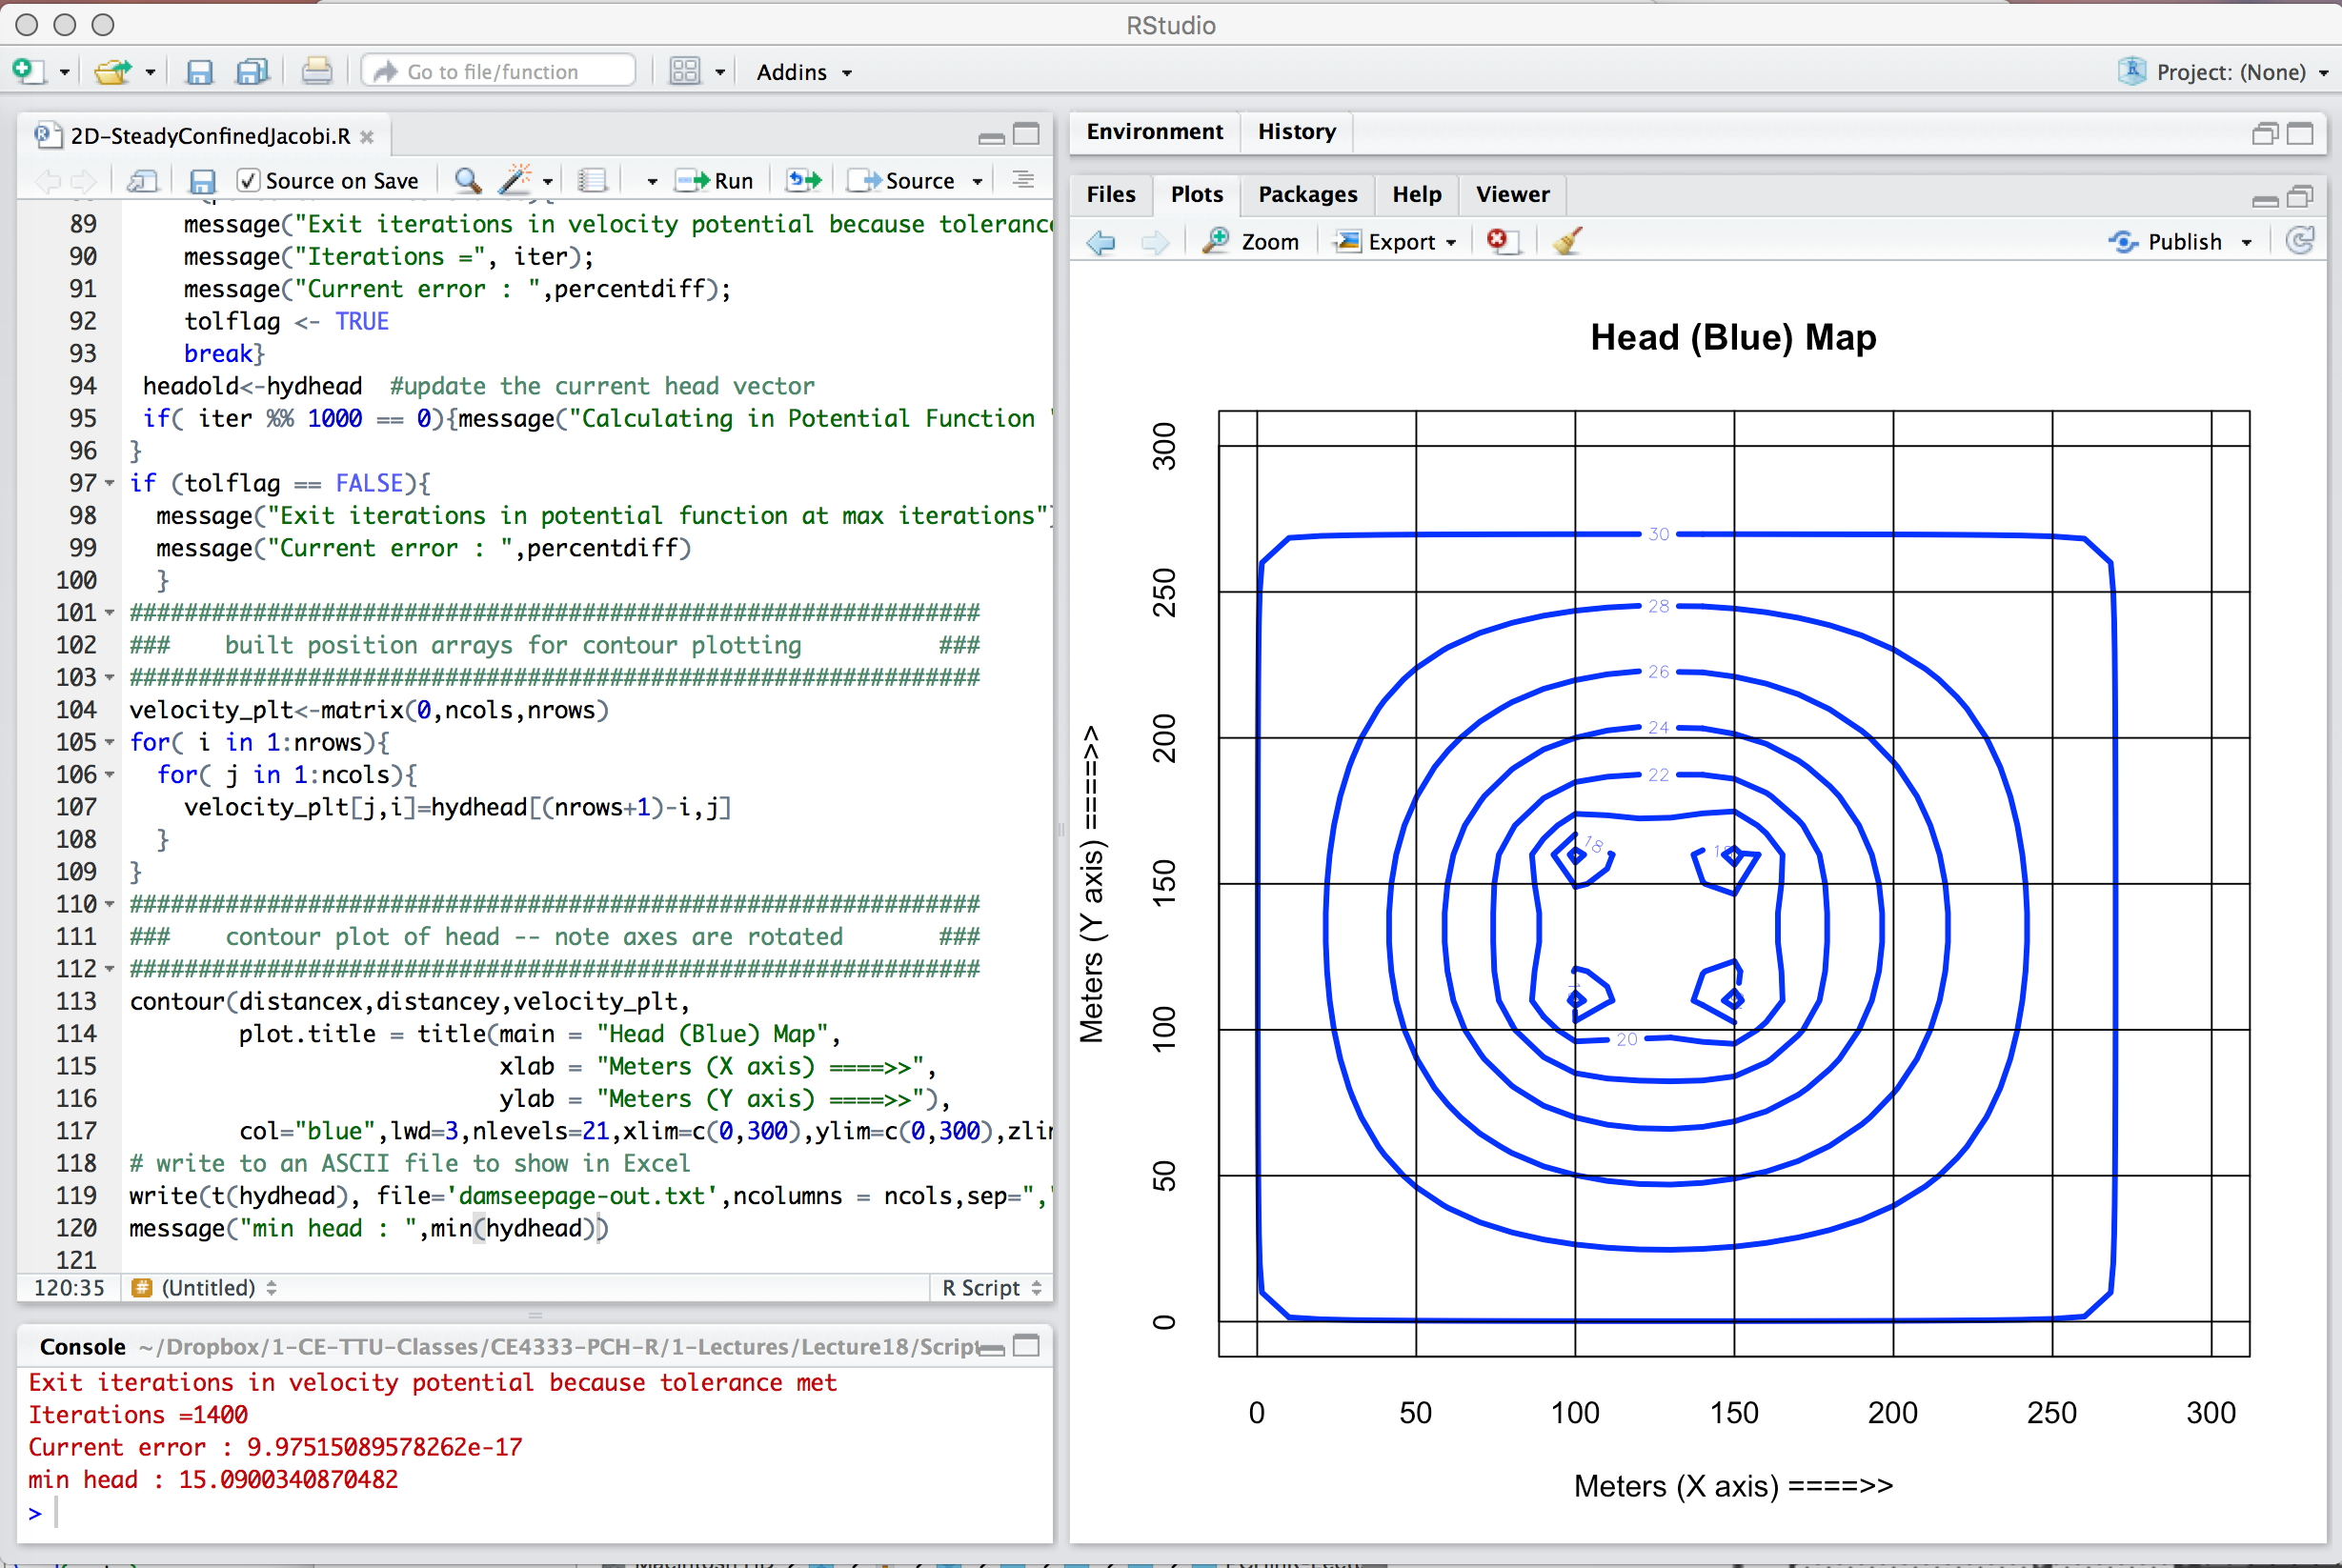
\includegraphics[width=6in]{./17-SteadyGroundwaterFlow/4WellsSteadyInR.jpg} 
   \caption{Rectangular aquifer with 4 wells}
   \label{fig:4WellsSteadyInR}
\end{figure}

The value for a single well is $0.430~\frac{m^3}{day}$ (using the units of hydraulic conductivity as a guide).  
If the goal was then to specify particular pumps, that flow value and the required lift would be used to specify and purchase pumps for the system. 

We will repeat he problem in the next section of the workbook, except the aquifer will be unconfined --- we expect different results, but will be able to re-use the input file.


\subsection{Unconfined Aquifer Flow}
Equation \ref{eqn:unconfined-mcb-2} is the meaningful part of Equation \ref{eqn:unconfined-mcb} from the previous chapter, which is our starting point for building unconfied flow computations.
\begin{equation}
S_{y} \Delta x  \frac{\partial h_i}{\partial t} = 
(K ~\overline{h}~ \frac{h_{i+1} - h_{i}}{\Delta x}) - 
(K ~\overline{h}~ \frac{h_{i} - h_{i-1}}{\Delta x})
\label{eqn:unconfined-mcb-2}
\end{equation}

\subsubsection{Finite-Difference Methods}
Here we will start with 2D flow -- if you have a 1D problem to solve, just make the model 3 cells wide in the un-needed axis and it will accomplish the same goal (and avoid having separate codes for different dimensions).

Here is the unconfined flow equation in 2 dimensions

\begin{equation}
\begin{matrix}
S_{y} \Delta x \Delta y \frac{\partial h_i}{\partial t} = 
[ K_{x} \Delta y ~\overline{h}~ \frac{h_{i-1,j} - h_{i,j}}{\Delta x} +
 K_{y} \Delta x ~\overline{h}~ \frac{h_{i,j-1} - h_{i,j}}{\Delta y}] - \\
~~~~~~~~~~\\
~~~~~~~~~~[ K_{x} \Delta y ~\overline{h}~ \frac{h_{i,j} - h_{i+1,j}}{\Delta x} +
K_{y} \Delta x ~\overline{h}~ \frac{h_{i,j} - h_{i,j+1}}{\Delta y} ]        
\end{matrix}        
\end{equation}

Next divide by the cell plan view area $\Delta x \Delta y$ to obtain a more compact form of the difference equation.

\begin{equation}
\begin{matrix}
S \frac{\partial h_i}{\partial t} = 
[\frac{1}{\Delta x} K_{x}~\overline{h}~ \frac{h_{i-1,j} - h_{i,j}}{\Delta x} +
 \frac{1}{\Delta y} K_{y}~\overline{h}~ \frac{h_{i,j-1} - h_{i,j}}{\Delta y}] - \\
~~~~~~~~~~\\
~~~~~~~~~~[ \frac{1}{\Delta x} K_{x}~\overline{h}~  \frac{h_{i,j} - h_{i+1,j}}{\Delta x} +
  \frac{1}{\Delta y}  K_{y}~\overline{h}~ \frac{h_{i,j} - h_{i,j+1}}{\Delta y} ]        
\end{matrix}        
\end{equation}

Again consider steady flow (we will do transient flows later on)

\begin{equation}
\begin{matrix}
0 = 
[\frac{1}{\Delta x} K_{x}~\overline{h}~ \frac{h_{i-1,j} - h_{i,j}}{\Delta x} +
 \frac{1}{\Delta y} K_{y}~\overline{h}~ \frac{h_{i,j-1} - h_{i,j}}{\Delta y}] - \\
~~~~~~~~~~\\
~~~~~~~~~~[ \frac{1}{\Delta x} K_{x}~\overline{h}~  \frac{h_{i,j} - h_{i+1,j}}{\Delta x} +
  \frac{1}{\Delta y}  K_{y}~\overline{h}~ \frac{h_{i,j} - h_{i,j+1}}{\Delta y} ]        
\end{matrix}        
\end{equation}

We will approximate the spatial variation of the $K~\overline{h}~$) as arithmetic mean values between two cells, so making the following definitions:

\begin{equation}
\begin{matrix}
A_{i,j} = \frac{1}{2 \Delta x^2}(K_{x,(i-1,j)} h_{i-1,j}+K_{x,(i,j)}h_{i,j}) \\ ~~ \\
B_{i,j} = \frac{1}{2 \Delta x^2}(K_{x,(i,j)}h_{i,j}+K_{x,(i+1,j)}h_{i+1,j})   \\ ~~ \\
C_{i,j} = \frac{1}{2 \Delta y^2}(K_{y,(i,j-1)}h_{i,j-1}+K_{y,(i,j)}h_{i,j})   \\ ~~ \\
D_{i,j} = \frac{1}{2 \Delta y^2}(K_{y,(i,j)}h_{i,j}+K_{y,(i,j+1)}h_{i,j+1})   \\ ~~ \\
\end{matrix}
\end{equation}

Substitution into the difference equation yields

\begin{equation}
0 = A_{i,j}h_{i-1,j} + B_{i,j}h_{i+1,j} - (A_{i,j}+B_{i,j}+C_{i,j}+D_{i,j})h_{i,j} + C_{i,j}h_{i,j-1} + D_{i,j}h_{i,j+1}
\end{equation}

As before we can explicitly write the cell equation for $h_{i,j}$ as, however the system is a bit non-linear as the $A,B,C,D$ coefficients are themselves functions of the cell values.

\begin{equation}
h_{i,j} = \frac{[A_{i,j}h_{i-1,j} + B_{i,j}h_{i+1,j} + C_{i,j}h_{i,j-1} + D_{i,j}h_{i,j+1}]}{[A_{i,j}+B_{i,j}+C_{i,j}+D_{i,j}]}
\end{equation}

This difference equation represents an approximation to the governing flow equation, the accuracy depending on the cell
size. Boundary conditions are applied directly into the analogs (another name for the difference equations) at appropriate
locations on the computational grid. Also as in the one-dimensional case we can generate solutions either by iteration or solving the resulting non-linear system.  
Fortunately theses kinds of systems are pretty well conditioned and one can usually compute the $A,B,C,D$ coefficients from the most recent value (in an iterative sense) of $h$ and proceeds as if the system is linear and it usually eventually converges.\footnote{The approach here is called the variable transmissivity approach as thats all i really did in the difference equation development -- as long as there is not too much curvature in the head distribution or dramatic changes in material properties in adjacent cells the Jacobi iteration method already employed will function, albeit slowly compared to more elaborate methods.  In this course we are satisfied with these relatively primitive constructs, and more sophisticated approaches are presented in the groundwater hydrology class taught by others.}

The method is again demonstrated by example.\\~\\
\textbf{Example 6: 4 Wells in a rectangular unconfined aquifer}~\\
Figure \ref{fig:4WellsSteadyUnconfined} is a rectangular aquifer with 4 wells as shown -- the drawing is identical to the previous example, except the aquifer is now an unconfined aquifer.  
The saturated thickness before the pumps are turned on is 30 meters.
The aquifer is surrounded with a constant head boundary of 30 meters.
The hydraulic conductivity is $K=0.033~m/day$.

Using a $10~meter~\times~10~meter$ grid spacing estimate the pumping rate in each well so that the head within the rectangular area defined by the well field is no greater than 15 meters.
In this example, the pumping rates will be quite a bit larger because the saturated thickness at the desired drawdown is 15 times larger that the previous example.
\begin{figure}[h!] %  figure placement: here, top, bottom, or page
   \centering
   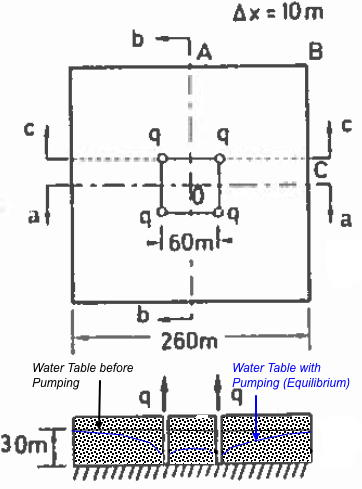
\includegraphics[height=6in]{./17-SteadyGroundwaterFlow/4WellsSteadyUnconfined.jpg} 
   \caption{Rectangular aquifer with 4 wells}
   \label{fig:4WellsSteadyUnconfined}
\end{figure}

Listing \ref{lst:UnconfinedSteady} is an \textbf{R} script that performs the indicated computations. 
Upon initial inspection it appears nearly identical to the confined flow script, except the $A,B,C,D$ computations are moved into the iteration loop, so they are updated after each iteration.  

Observe that the $\Delta z$ value is still read into the script, but never used.
I am being somewhat lazy here; however it illustrates a code development protocol to re-use as much code as possible until the program functions as desired, then we could go back and delete unused components.
I choose to retain the $\Delta z$ so I would only have to change the input file pumping array and not create an entirely new input file structure.  
As stated earlier, as the problems get big, we would write scripts that build the input files before we run the computation engines.
~\newpage
\begin{lstlisting}[caption= \textbf{R} script implementing unconfined aquifer flow computations with wells and generalized boundary conditions. , label=lst:UnconfinedSteady]
# 2D Steady UnConfined -- With Boundary Arrays -- And Pumping Array
# 2D Aquifer Flow Model using Jacobi Iteration
# deallocate memory
rm(list=ls())
zz <- file("wellfield2.dat", "r") # Open a connection named zz to file named input.dat
# read the simulation conditons
deltax <-as.numeric(readLines(zz, n = 1, ok = TRUE, warn = TRUE,encoding = "unknown", skipNul = FALSE))
deltay <-as.numeric(readLines(zz, n = 1, ok = TRUE, warn = TRUE,encoding = "unknown", skipNul = FALSE))
deltaz <-as.numeric(readLines(zz, n = 1, ok = TRUE, warn = TRUE,encoding = "unknown", skipNul = FALSE))
# here we retain deltaz but will not use it, we assume head is the deltaz
nrows <-as.numeric(readLines(zz, n = 1, ok = TRUE, warn = TRUE,encoding = "unknown", skipNul = FALSE))
ncols <-as.numeric(readLines(zz, n = 1, ok = TRUE, warn = TRUE,encoding = "unknown", skipNul = FALSE))
tolerance <- as.numeric(readLines(zz, n = 1, ok = TRUE, warn = TRUE,encoding = "unknown", skipNul = FALSE))
maxiter <- as.numeric(readLines(zz, n = 1, ok = TRUE, warn = TRUE,encoding = "unknown", skipNul = FALSE))
distancex <- (readLines(zz, n = 1, ok = TRUE, warn = TRUE,encoding = "unknown", skipNul = FALSE))
distancey <- (readLines(zz, n = 1, ok = TRUE, warn = TRUE,encoding = "unknown", skipNul = FALSE))
# add boundary conditions 0= fixed head, 1= no flow
boundarytop <- (readLines(zz, n = 1, ok = TRUE, warn = TRUE,encoding = "unknown", skipNul = FALSE))
boundarybottom <- (readLines(zz, n = 1, ok = TRUE, warn = TRUE,encoding = "unknown", skipNul = FALSE))
boundaryleft <- (readLines(zz, n = 1, ok = TRUE, warn = TRUE,encoding = "unknown", skipNul = FALSE))
boundaryright <- (readLines(zz, n = 1, ok = TRUE, warn = TRUE,encoding = "unknown", skipNul = FALSE))
hydhead <-(readLines(zz, n = nrows, ok = TRUE, warn = TRUE,encoding = "unknown", skipNul = FALSE))
# hydhead is now the initial condition array #
hydcondx <-(readLines(zz, n = nrows, ok = TRUE, warn = TRUE,encoding = "unknown", skipNul = FALSE))
hydcondy <-(readLines(zz, n = nrows, ok = TRUE, warn = TRUE,encoding = "unknown", skipNul = FALSE))
# add pumping array
pumping <-(readLines(zz, n = nrows, ok = TRUE, warn = TRUE,encoding = "unknown", skipNul = FALSE))
close(zz)
# split the multiple column strings into numeric components for a vector
distancex <-as.numeric(unlist(strsplit(distancex,split=" ")))
distancey <-as.numeric(unlist(strsplit(distancey,split=" ")))
boundarytop <-as.numeric(unlist(strsplit(boundarytop,split=" ")))
boundarybottom <-as.numeric(unlist(strsplit(boundarybottom,split=" ")))
boundaryleft <-as.numeric(unlist(strsplit(boundaryleft,split=" ")))
boundaryright <-as.numeric(unlist(strsplit(boundaryright,split=" ")))
hydhead <-as.numeric(unlist(strsplit(hydhead,split=" ")))
hydcondx <-as.numeric(unlist(strsplit(hydcondx,split=" ")))
hydcondy <-as.numeric(unlist(strsplit(hydcondy,split=" ")))
pumping <-as.numeric(unlist(strsplit(pumping,split=" ")))
# convert the numeric vectors into matrices for easier indexing
hydhead <- matrix(hydhead,nrow=nrows,ncol=ncols,byrow = TRUE)
hydcondx <-matrix(hydcondx,nrow=nrows,ncol=ncols,byrow = TRUE)
hydcondy <-matrix(hydcondy,nrow=nrows,ncol=ncols,byrow = TRUE)
pumping <-matrix(pumping,nrow=nrows,ncol=ncols,byrow = TRUE)
# here we perform the velocity potential calculations
# allocate the transmissivity arrays
amat<-matrix(0,nrows,ncols) 
bmat<-matrix(0,nrows,ncols) 
cmat<-matrix(0,nrows,ncols)
dmat<-matrix(0,nrows,ncols)
# allocate and build the pumping array
qrat<-matrix(0,nrows,ncols)
for(irow in 2:(nrows-1)){
  for(jcol in 2:(ncols-1)){
    qrat[irow,jcol]<-(-1.0)*pumping[irow,jcol]/(deltax*deltay)
  }
}
headold <- hydhead # copy the head array, used to test for stopping 
tolflag <- FALSE
for (iter in 1:maxiter){
# built the variable transmissivity arrays
  for(irow in 2:(nrows-1)){
    for(jcol in 2:(ncols-1)){
      amat[irow,jcol]<-((hydcondx[irow-1,jcol  ]*hydhead[irow-1,jcol  ]
                  +hydcondx[irow  ,jcol  ]*hydhead[irow  ,jcol  ]))/(2.0*deltax^2)
      
      bmat[irow,jcol]<-((hydcondx[irow  ,jcol  ]*hydhead[irow  ,jcol  ]
                  +hydcondx[irow+1,jcol  ]*hydhead[irow+1,jcol  ]))/(2.0*deltax^2)
      
      cmat[irow,jcol]<-((hydcondy[irow  ,jcol-1]*hydhead[irow  ,jcol-1]
                  +hydcondy[irow  ,jcol  ]*hydhead[irow  ,jcol  ]))/(2.0*deltay^2)
      
      dmat[irow,jcol]<-((hydcondy[irow  ,jcol  ]*hydhead[irow  ,jcol  ]
                  +hydcondy[irow  ,jcol+1]*hydhead[irow  ,jcol+1]))/(2.0*deltay^2)
      
    }
  }  
  
# Boundary Conditions
# Top and Bottom
for(jcol in 1:ncols){
    if(boundarytop[jcol] == 0){hydhead[1,jcol]<-hydhead[2,jcol]} #no-flow at top
    if(boundarybottom[jcol] == 0){hydhead[nrows,jcol]<-hydhead[nrows-1,jcol]} #no-flow at bottom
    # otherwise values are fixed head
}
for(irow in 1:nrows){
    if(boundaryleft[irow] == 0){hydhead[irow,1]<-hydhead[irow,2]} #no-flow at left
    if(boundaryright[irow] == 0){hydhead[irow,ncols]<-hydhead[irow,ncols-1]} #no-flow at right
    # otherwise values are fixed head
}
  for (irow in 2:(nrows-1)){
    for (jcol in 2:(ncols-1)){
      hydhead[irow,jcol] <- 
          (                       qrat[irow,jcol] +
           amat[irow,jcol]*hydhead[irow-1,jcol  ] +
           bmat[irow,jcol]*hydhead[irow+1,jcol  ] +
           cmat[irow,jcol]*hydhead[irow  ,jcol-1] +
           dmat[irow,jcol]*hydhead[irow  ,jcol+1]  )/
        (amat[irow,jcol]+bmat[irow,jcol]+cmat[irow,jcol]+dmat[irow,jcol])
    }
  }
  # test for stopping iterations
  percentdiff <- sum((hydhead-headold)^2)
  if (percentdiff < tolerance){
    message("Exit iterations in velocity potential because tolerance met");
    message("Iterations =", iter);
    message("Current error : ",percentdiff);
    tolflag <- TRUE
    break}
 headold<-hydhead  #update the current head vector
 if( iter %% 1000 == 0){message("Calculating in Potential Function ",iter," of ",maxiter, " iterations")}
}
if (tolflag == FALSE){
  message("Exit iterations in potential function at max iterations")
  message("Current error : ",percentdiff)
  }
##############################################################
###    built position arrays for contour plotting          ###
##############################################################
velocity_plt<-matrix(0,ncols,nrows) 
for( i in 1:nrows){
  for( j in 1:ncols){
    velocity_plt[j,i]=hydhead[(nrows+1)-i,j]
  }
}
##############################################################
###    contour plot of head -- note axes are rotated       ###
##############################################################
contour(distancex,distancey,velocity_plt,
        plot.title = title(main = "Head (Blue) Map",
                           xlab = "Meters (X axis) ====>>", 
                           ylab = "Meters (Y axis) ====>>"),
        col="blue",lwd=3,nlevels=21,xlim=c(0,300),ylim=c(0,300),zlim=c(-1,40),tck=1)
# write to an ASCII file to show in Excel
write(t(hydhead), file='damseepage-out.txt',ncolumns = ncols,sep=",") 
message("min head : ",min(hydhead))
\end{lstlisting}

Listing \ref{lst:wellfield2} is the relevant portion of the input file for the example.  The remainder of the file is unchanged from the previous example (hence the reason I retained the $\Delta z$ variable).
\begin{lstlisting}[caption= Relevant portion of input file for unconfined flow example.  Only the pumping values are different. , label=lst:wellfield2]
...........
0.000 0.000 0.000 0.000 0.000 0.000 0.000 0.000 0.000 0.000 0.000 0.000 0.000 0.000 0.000 0.000 0.000 0.000 0.000 0.000 0.000 0.000 0.000 0.000 0.000 0.000 0.000 0.000
0.000 0.000 0.000 0.000 0.000 0.000 0.000 0.000 0.000 0.000 9.500 0.000 0.000 0.000 0.000 9.500 0.000 0.000 0.000 0.000 0.000 0.000 0.000 0.000 0.000 0.000 0.000 0.000
0.000 0.000 0.000 0.000 0.000 0.000 0.000 0.000 0.000 0.000 0.000 0.000 0.000 0.000 0.000 0.000 0.000 0.000 0.000 0.000 0.000 0.000 0.000 0.000 0.000 0.000 0.000 0.000
0.000 0.000 0.000 0.000 0.000 0.000 0.000 0.000 0.000 0.000 0.000 0.000 0.000 0.000 0.000 0.000 0.000 0.000 0.000 0.000 0.000 0.000 0.000 0.000 0.000 0.000 0.000 0.000
0.000 0.000 0.000 0.000 0.000 0.000 0.000 0.000 0.000 0.000 0.000 0.000 0.000 0.000 0.000 0.000 0.000 0.000 0.000 0.000 0.000 0.000 0.000 0.000 0.000 0.000 0.000 0.000
0.000 0.000 0.000 0.000 0.000 0.000 0.000 0.000 0.000 0.000 0.000 0.000 0.000 0.000 0.000 0.000 0.000 0.000 0.000 0.000 0.000 0.000 0.000 0.000 0.000 0.000 0.000 0.000
0.000 0.000 0.000 0.000 0.000 0.000 0.000 0.000 0.000 0.000 9.500 0.000 0.000 0.000 0.000 9.500 0.000 0.000 0.000 0.000 0.000 0.000 0.000 0.000 0.000 0.000 0.000 0.000
0.000 0.000 0.000 0.000 0.000 0.000 0.000 0.000 0.000 0.000 0.000 0.000 0.000 0.000 0.000 0.000 0.000 0.000 0.000 0.000 0.000 0.000 0.000 0.000 0.000 0.000 0.000 0.000
.............
\end{lstlisting}

Figure \ref{fig:4WellsSteadyUnconfinedInR} is a screen capture of the example implemented in \textbf{R}.
The plot is practically the same as in the previous example (in fact of the labels were not moved on the contour lines, the figures would look identical) however the pumping rate is 20 times larger for apparently the same head distribution --- so if the dewatering effort were in an unconfined aquifer, perhaps for an excavation for a foundation, choosing the correct conditions would be kind of important.\footnote{Well more than ``kind-of''  --- absolutely vital to size the dewatering points and pumps.}

\begin{figure}[h!] %  figure placement: here, top, bottom, or page
   \centering
   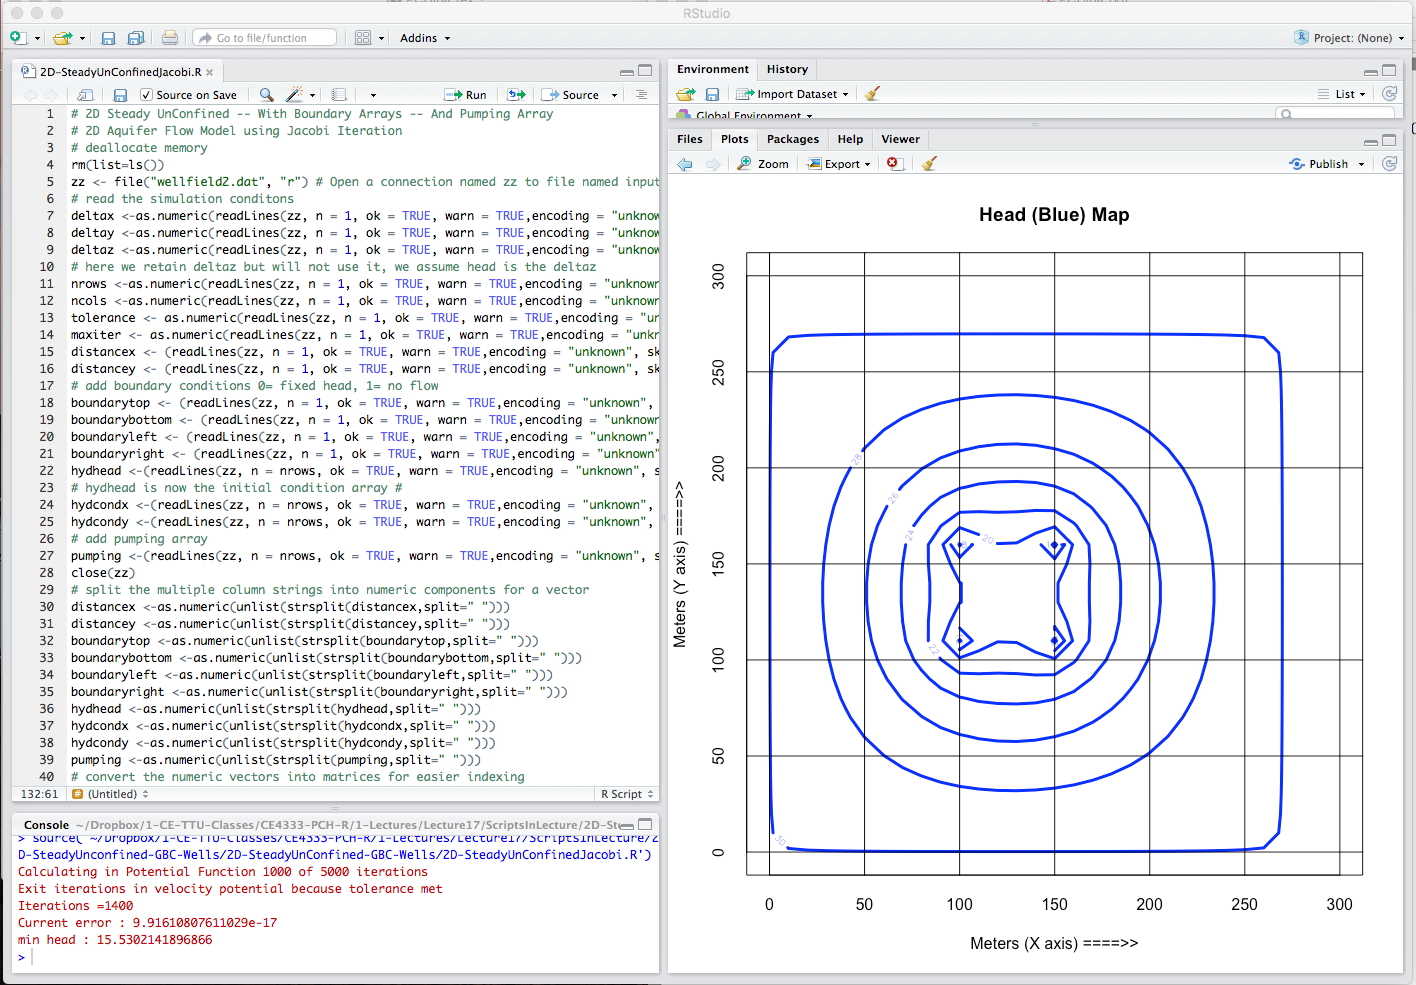
\includegraphics[width=6in]{./17-SteadyGroundwaterFlow/4WellsSteadyUnconfinedInR.jpg} 
   \caption{Rectangular unconfined aquifer with 4 wells.  Solution and plotting using \textbf{R}}
   \label{fig:4WellsSteadyUnconfinedInR}
\end{figure}


As a quick summary of this chapter we started with a 1D situation and built a couple of finite-difference models to illustrate the use of \texttt{solve(...)} and our homebrew Jacobi iteration method.  Next we progressed to a 2D situation (it can either be a slice or a layer) and used the Jacobi iteration method.  Using a formal linear solver would also work quite well, but the matrix assembly is a bit tedious -- so that was left for future editions of this book.   Once we had our 2D computation engine working we extended capability by adding generalized boundary condition capability to the exterior boundaries (the same can be done for interior cells -- the matrix assembly logic is awkward, so that too is left for future editions).   Once the generalized boundary modification was built, we then added a recharge/pumping capability.  This last model is functionally useful (although it needs testing against known solutions to detect any coding errors).   To complete the chapter, a simple modification using the variable transmissivity construct allowed us to extend our capability to unconfined aquifers.  The next chapter will illustrate unsteady flow where the left hand side of the PDEs is no longer zero.
\clearpage

\subsection{Exercises}
\begin{enumerate}
\item Repeat Example 5 (4 Wells in a Confined Aquifer) with an aquifer thickness of 10 meters and determine:
\begin{enumerate}
\item The pumping rate in each well that produces a minimum aquifer head of 15 meters.
\item Produce a contour plot of this solution and report the required pumping rate in cubic meters per day.
\item Plot the head in a elevation/profile view (vertical slice into the aquifer -- section a--a in the sketch) that passes through the middle of the aquifer (between the wells) running from left to right.
\end{enumerate}


\item Figure \ref{fig:Obleo} is a plan view map of the hydrologic setting of the OBLEO aquifer.  
The aquifer is an unconfined aquifer with a single well, P-1, in its geographic center.  
The aquifer is bounded to the North and South by mountains, and the East and West by two large lakes.  
The water elevation in each lake is 100.0 meters above some datum, while the ground elevation at the well is 200.0 meters above the same datum.

\begin{figure}[h!] %  figure placement: here, top, bottom, or page
   \centering
   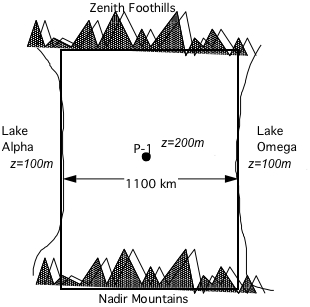
\includegraphics[width=6in]{./17-SteadyGroundwaterFlow/Obleo.jpg} 
   \caption{Obleo Aquifer Setting (Plan View)}
   \label{fig:Obleo}
\end{figure}

Rainfall records indicate that recharge to the subsurface is approximately 250 mm/yr.  
The aquifer is homogeneous and isotropic ($K_x = K_y$) with a hydraulic conductivity value of $K=100m/day$, and a specific yield $S_y~=0.25$.  The example constructs a computer model to help determine the safe yield of the aquifer - assume minimum permissible saturated thickness is 50 m.
\begin{enumerate}
\item Write/Modify an \textbf{R} script to include a recharge array (in addition to a pumping array).  
Take care that you use the correct sign when adding this array into the computation engine.
\item What kind of boundary condition makes sense for the two lakes?
\item What kind of boundary condition makes sense for the two mountain ranges?
\item Build an input file in the structure used in the examples.  
Use a grid size of 100km X 100km\footnote{Yes, i am aware that this aquifer is over 600 miles between the lakes!}.
\item Compute the head distribution and produce a contour plot with just recharge (no pumping).
\item Plot the head in a elevation/profile view (vertical slice into the aquifer) that passes through the well running from West to East. (Lake to Lake).
\item Compute the head distribution with recharge \textbf{and} pumping at a rate that produces a minimum saturated thickness of about 50 meters.
\item Produce a contour plot of this solution and report the required pumping rate in cubic meters per day. 
\item Plot the head in a elevation/profile view (vertical slice into the aquifer) that passes through the well running from West to East. (Lake to Lake).
\item Capture these plots into a brief report where you compare the aquifer conditions before pumping and during pumping.
\end{enumerate}

\end{enumerate}
%%%%%%%%%%%%%%%%%%%%%%%%%%%%%%%%%%%%%%%%%%%%%%%%%%%%%%